\begin{figure}[ht!]
     \centering
    \caption{Partial dependence plot (SHAP) for 87 countries and nine clusters}
    \label{fig:5b}
     \begin{subfigure}[b]{\textwidth}
         \centering
         \caption{Partial dependence plot (SHAP) for Argentina (cluster A)}
         \label{fig:5b_ARG}
         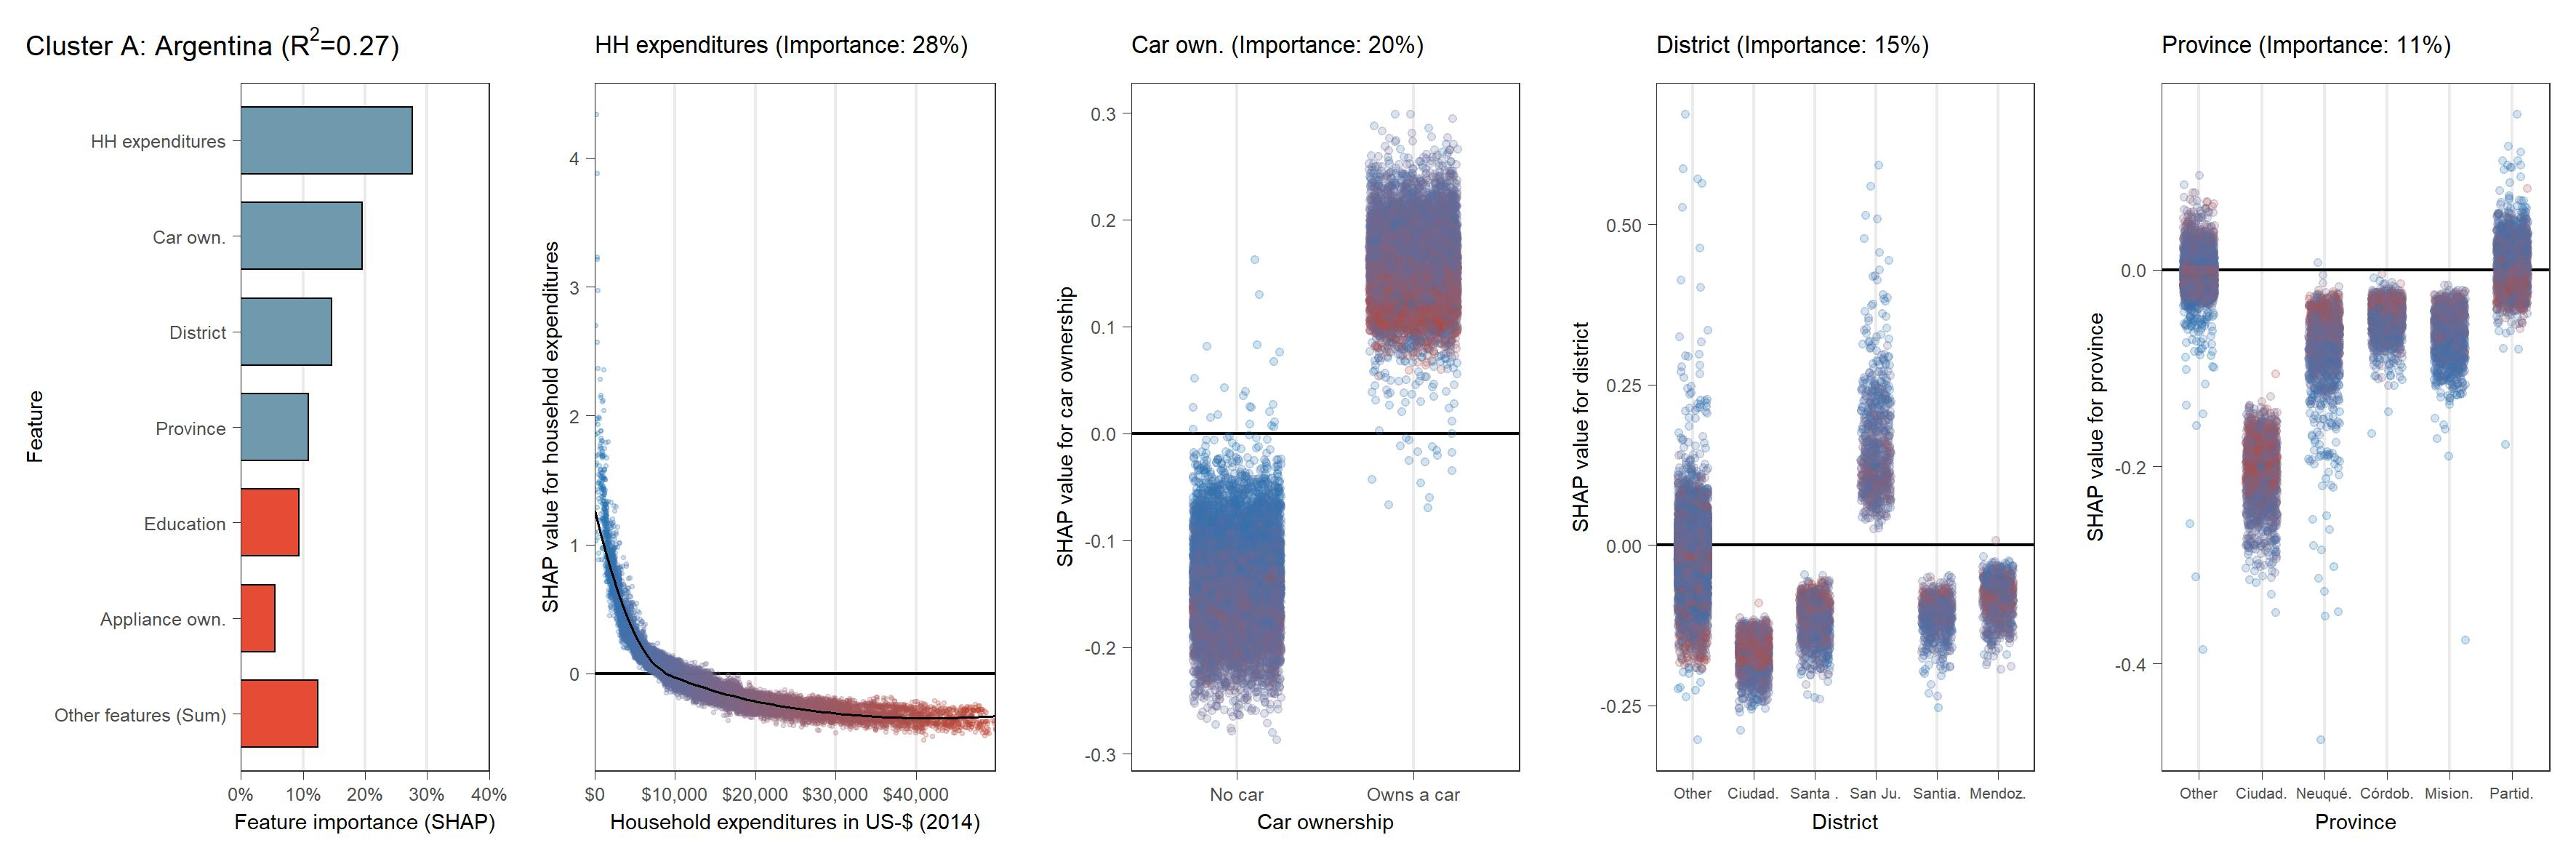
\includegraphics[width=\textwidth]{Figure 5b/Figure_5b_ARG} 
     \end{subfigure}
    \\
    \vspace{0.5cm}
     \begin{subfigure}[b]{\textwidth}
         \centering
         \caption{Partial dependence plot (SHAP) for Austria (cluster A)}
         \label{fig:5b_AUT}
         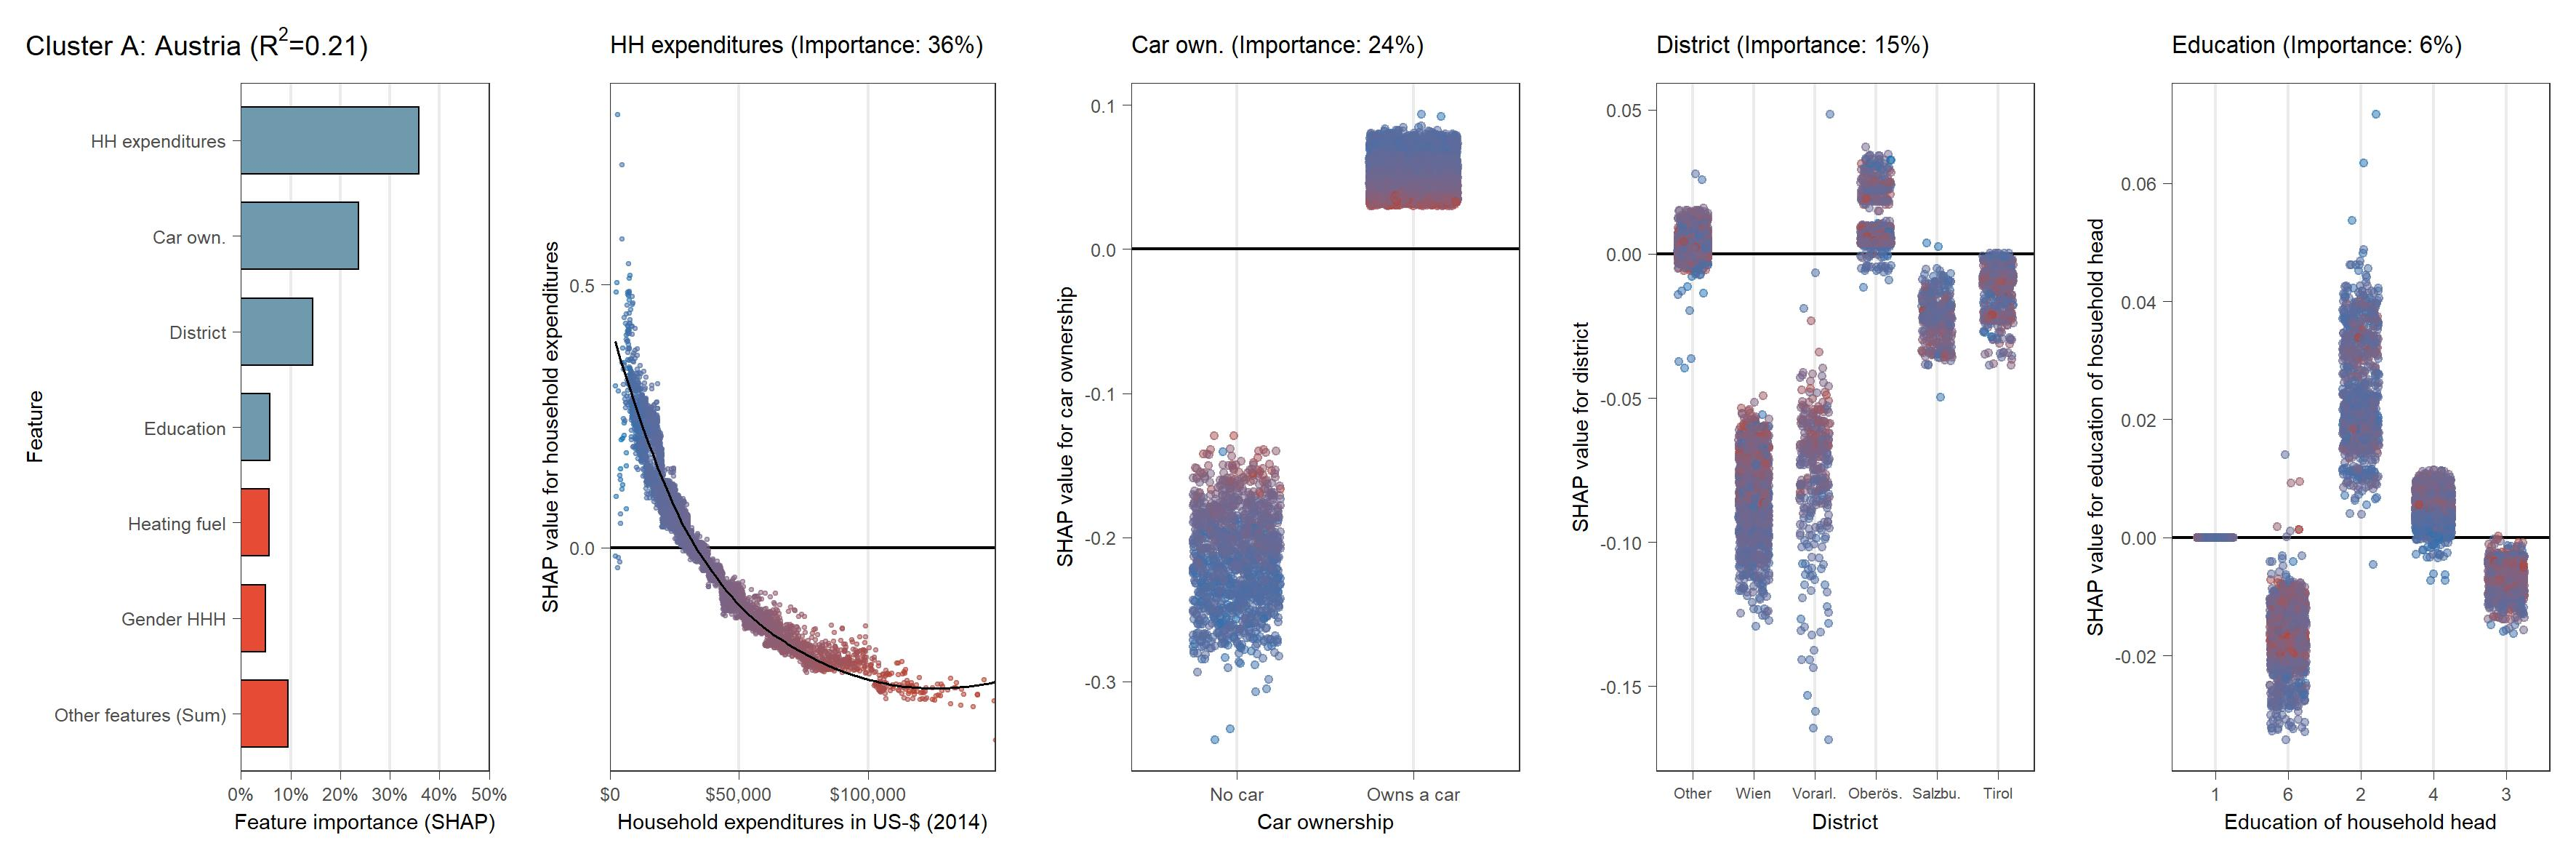
\includegraphics[width=\textwidth]{Figure 5b/Figure_5b_AUT}    \end{subfigure}
    \\
    \vspace{0.5cm}
     \begin{subfigure}[b]{1\textwidth}
     \centering
         \caption{Partial dependence plot (SHAP) for Belgium (cluster A)}
         \label{fig:5b_BEL}
         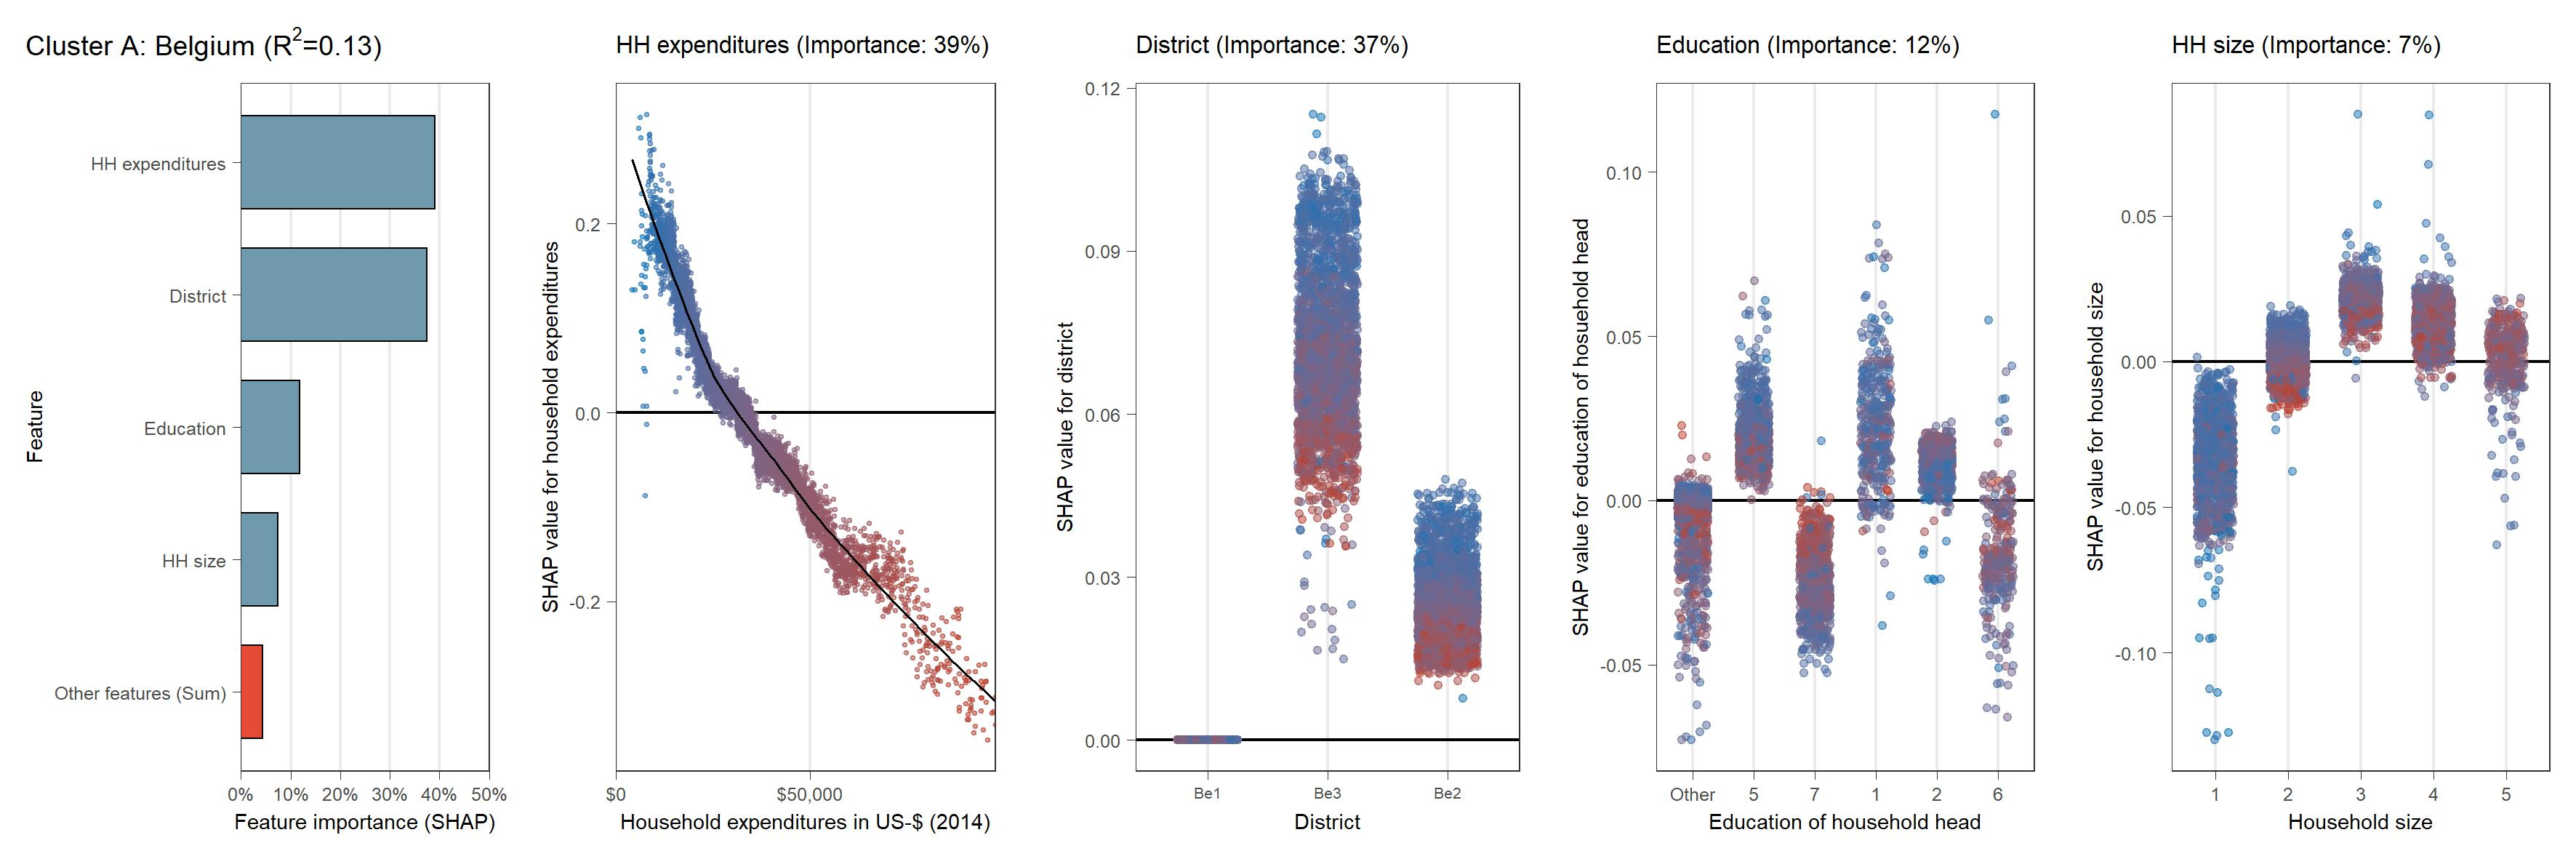
\includegraphics[width=\textwidth]{Figure 5b/Figure_5b_BEL} 
         \end{subfigure}
     \\
     \vspace{0.5cm}
        \begin{subcaption2}
     This figure shows SHAP-values for predicting carbon intensity over feature values for 87 countries in order of nine country-clusters and silhouette width. The bar chart displays normalized average absolute SHAP-values for all features. Features with less than 3\% of normalized SHAP-values are subsumed as "Other features (Sum)". Charts show SHAP-values over total household expenditures for all countries and for the three most important features in each country besides total household expenditures. Colors represent household expenditures with blue (red) colors indicating lower (higher) household expenditures.
     \end{subcaption2}
     \end{figure}
     
\begin{figure}[ht!]\ContinuedFloat
    \centering
   \begin{subfigure}[b]{\textwidth}
   \centering
         \caption{Partial dependence plot (SHAP) for Bulgaria (cluster A)}
         \label{fig:5b_BGR}
         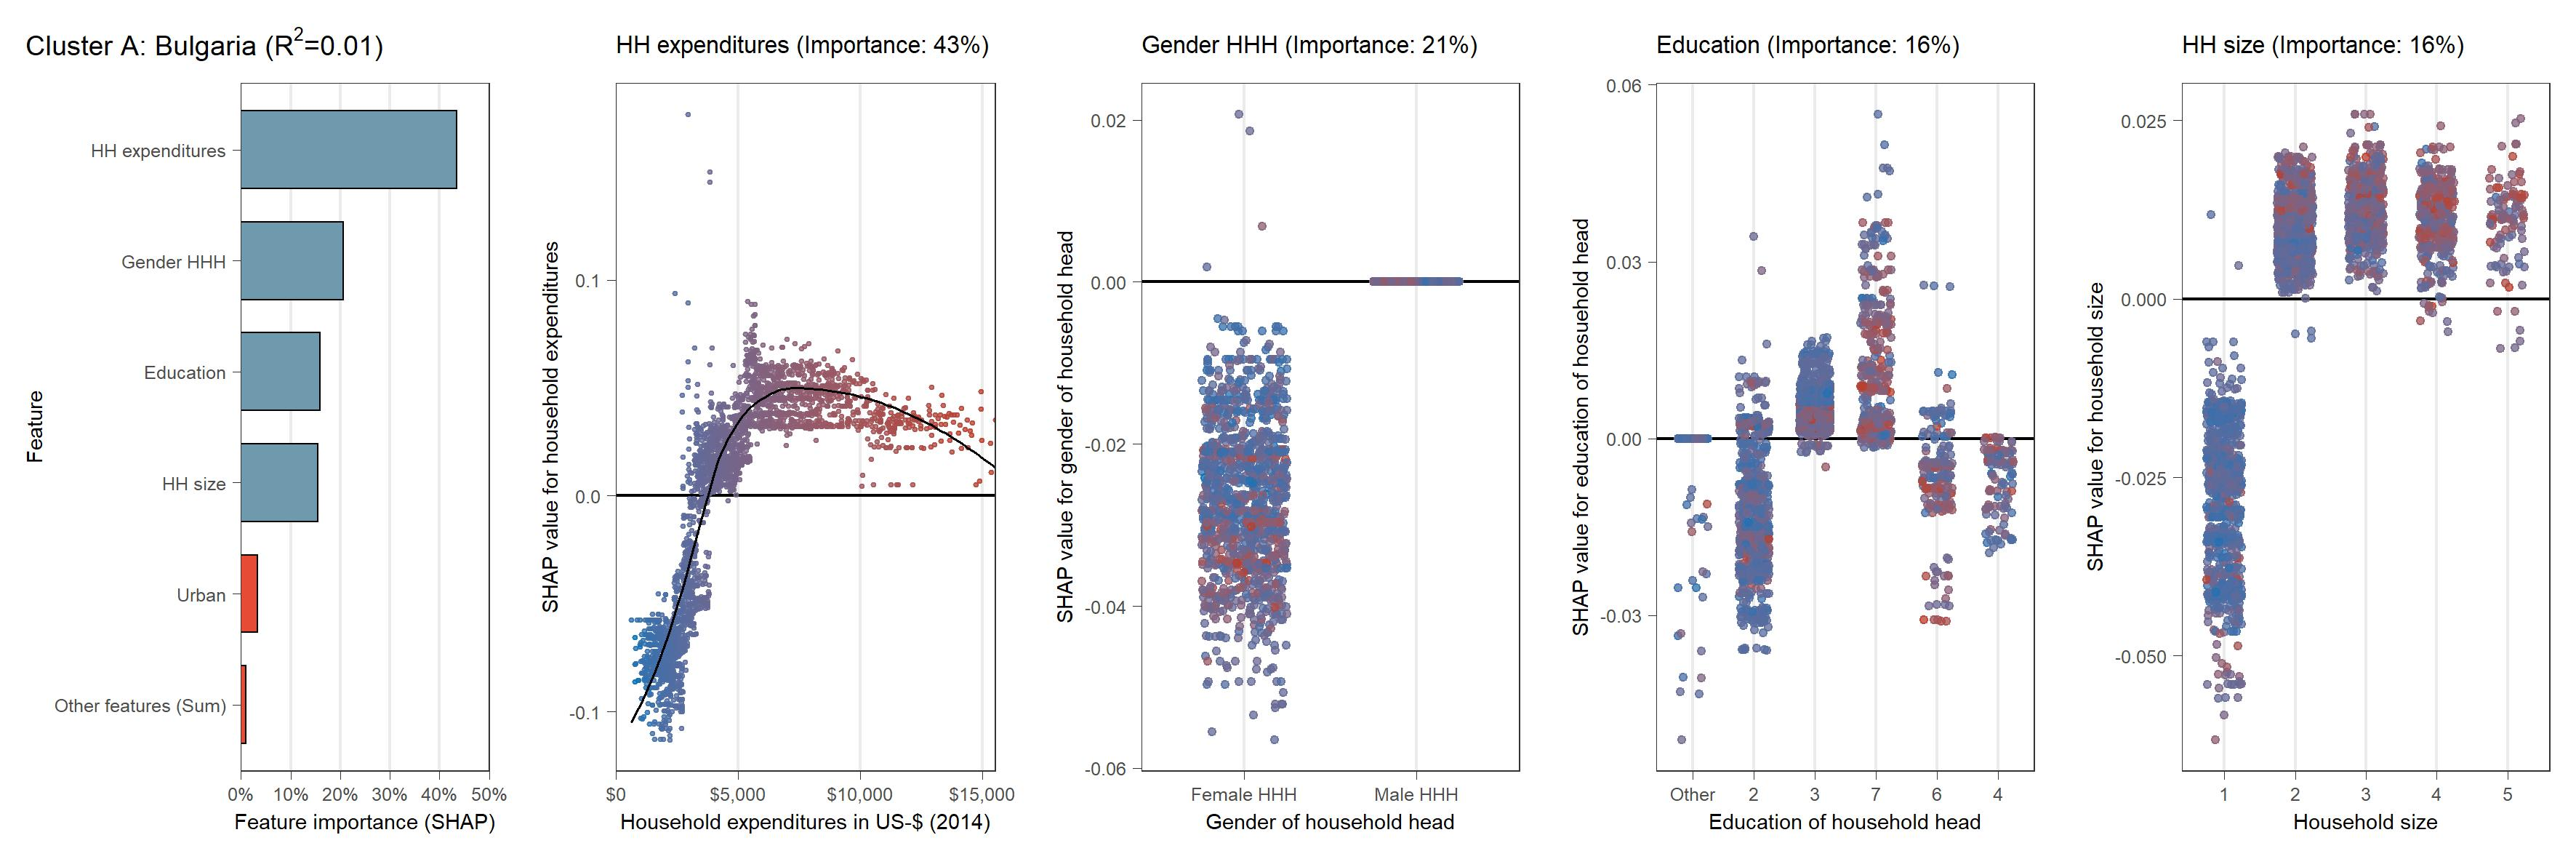
\includegraphics[width=\textwidth]{Figure 5b/Figure_5b_BGR}
         \end{subfigure}
    \\
    \vspace{0.5cm}
   \begin{subfigure}[b]{\textwidth}
   \centering
         \caption{Partial dependence plot (SHAP) for Brazil (cluster A)}
         \label{fig:5b_BRA}
         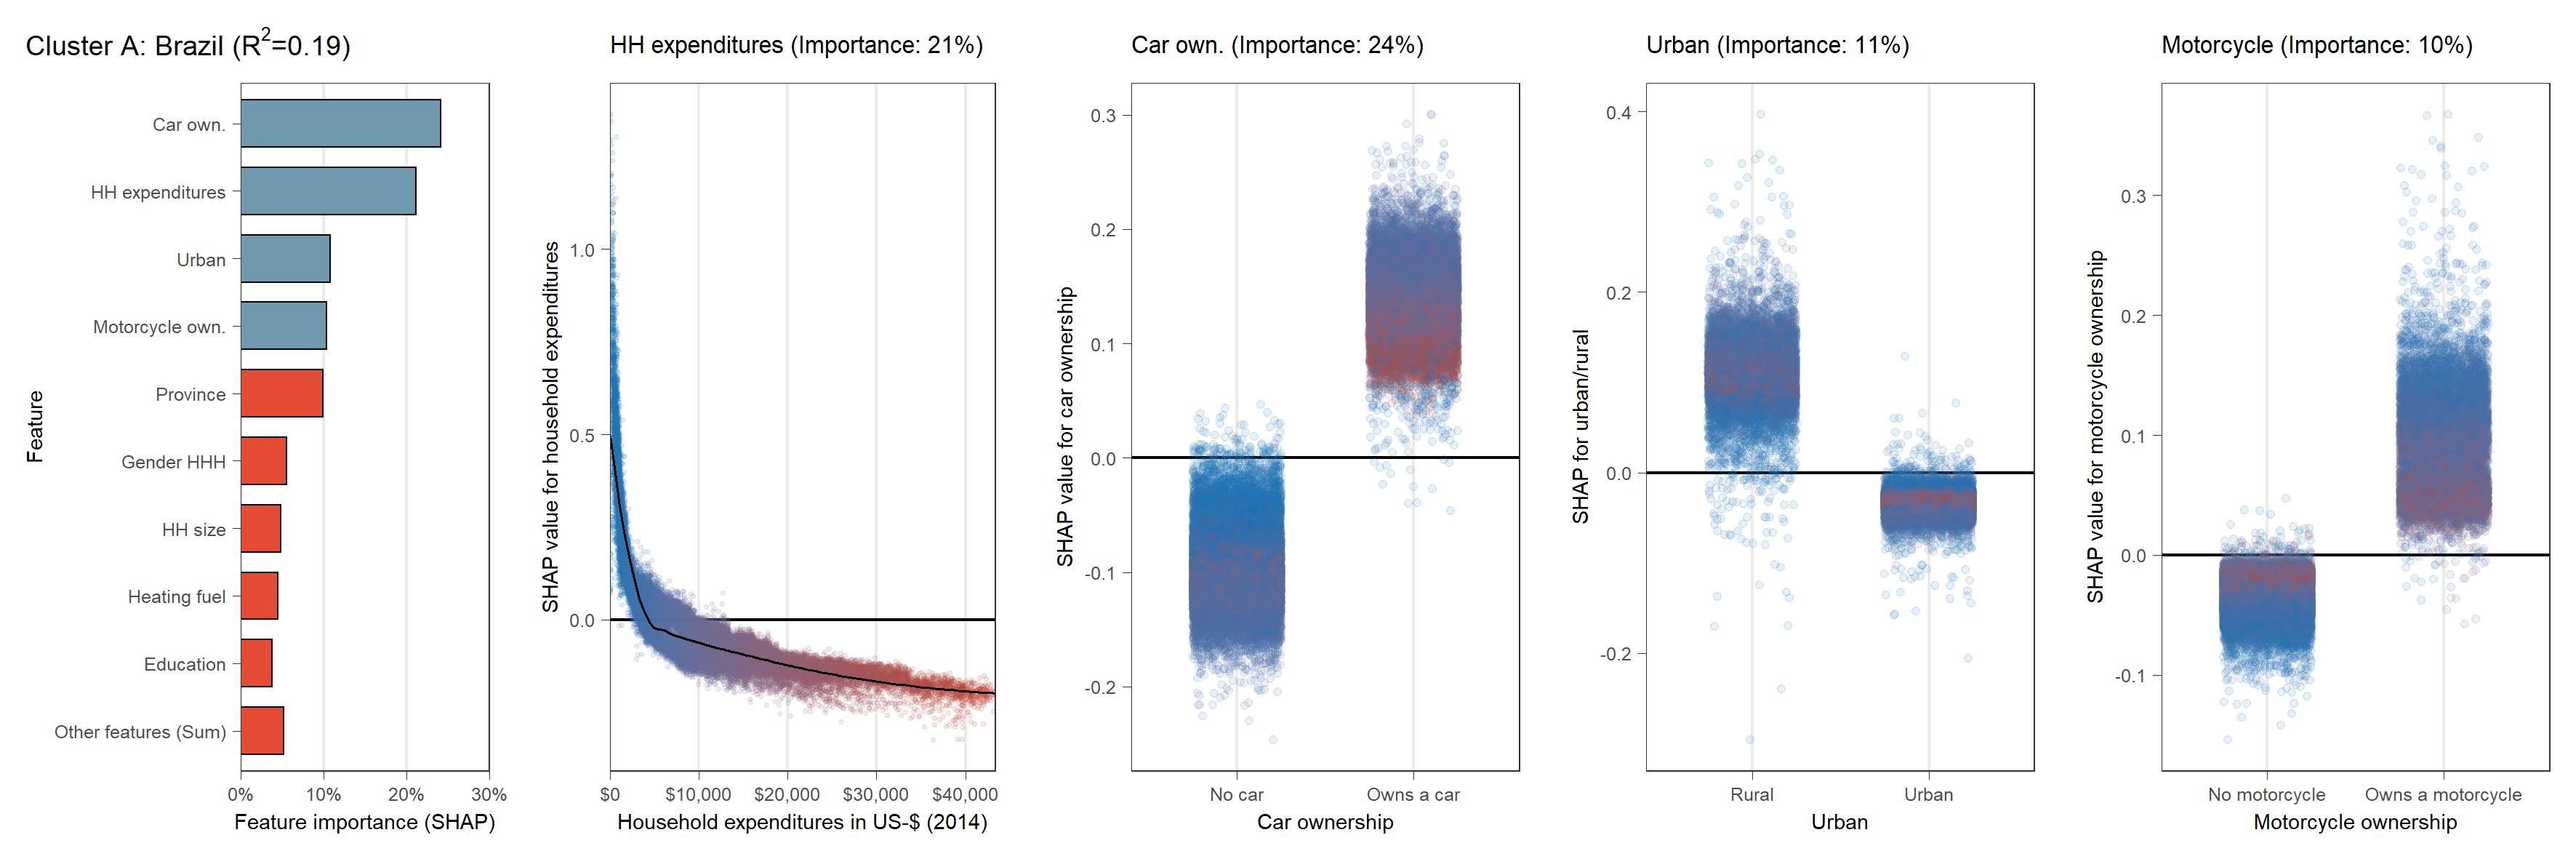
\includegraphics[width=\textwidth]{Figure 5b/Figure_5b_BRA} 
         \end{subfigure}
    \\
    \vspace{0.5cm}
   \begin{subfigure}[b]{\textwidth}
         \centering
         \caption{Partial dependence plot (SHAP) for Barbados (cluster A)}
         \label{fig:5b_BRB}
         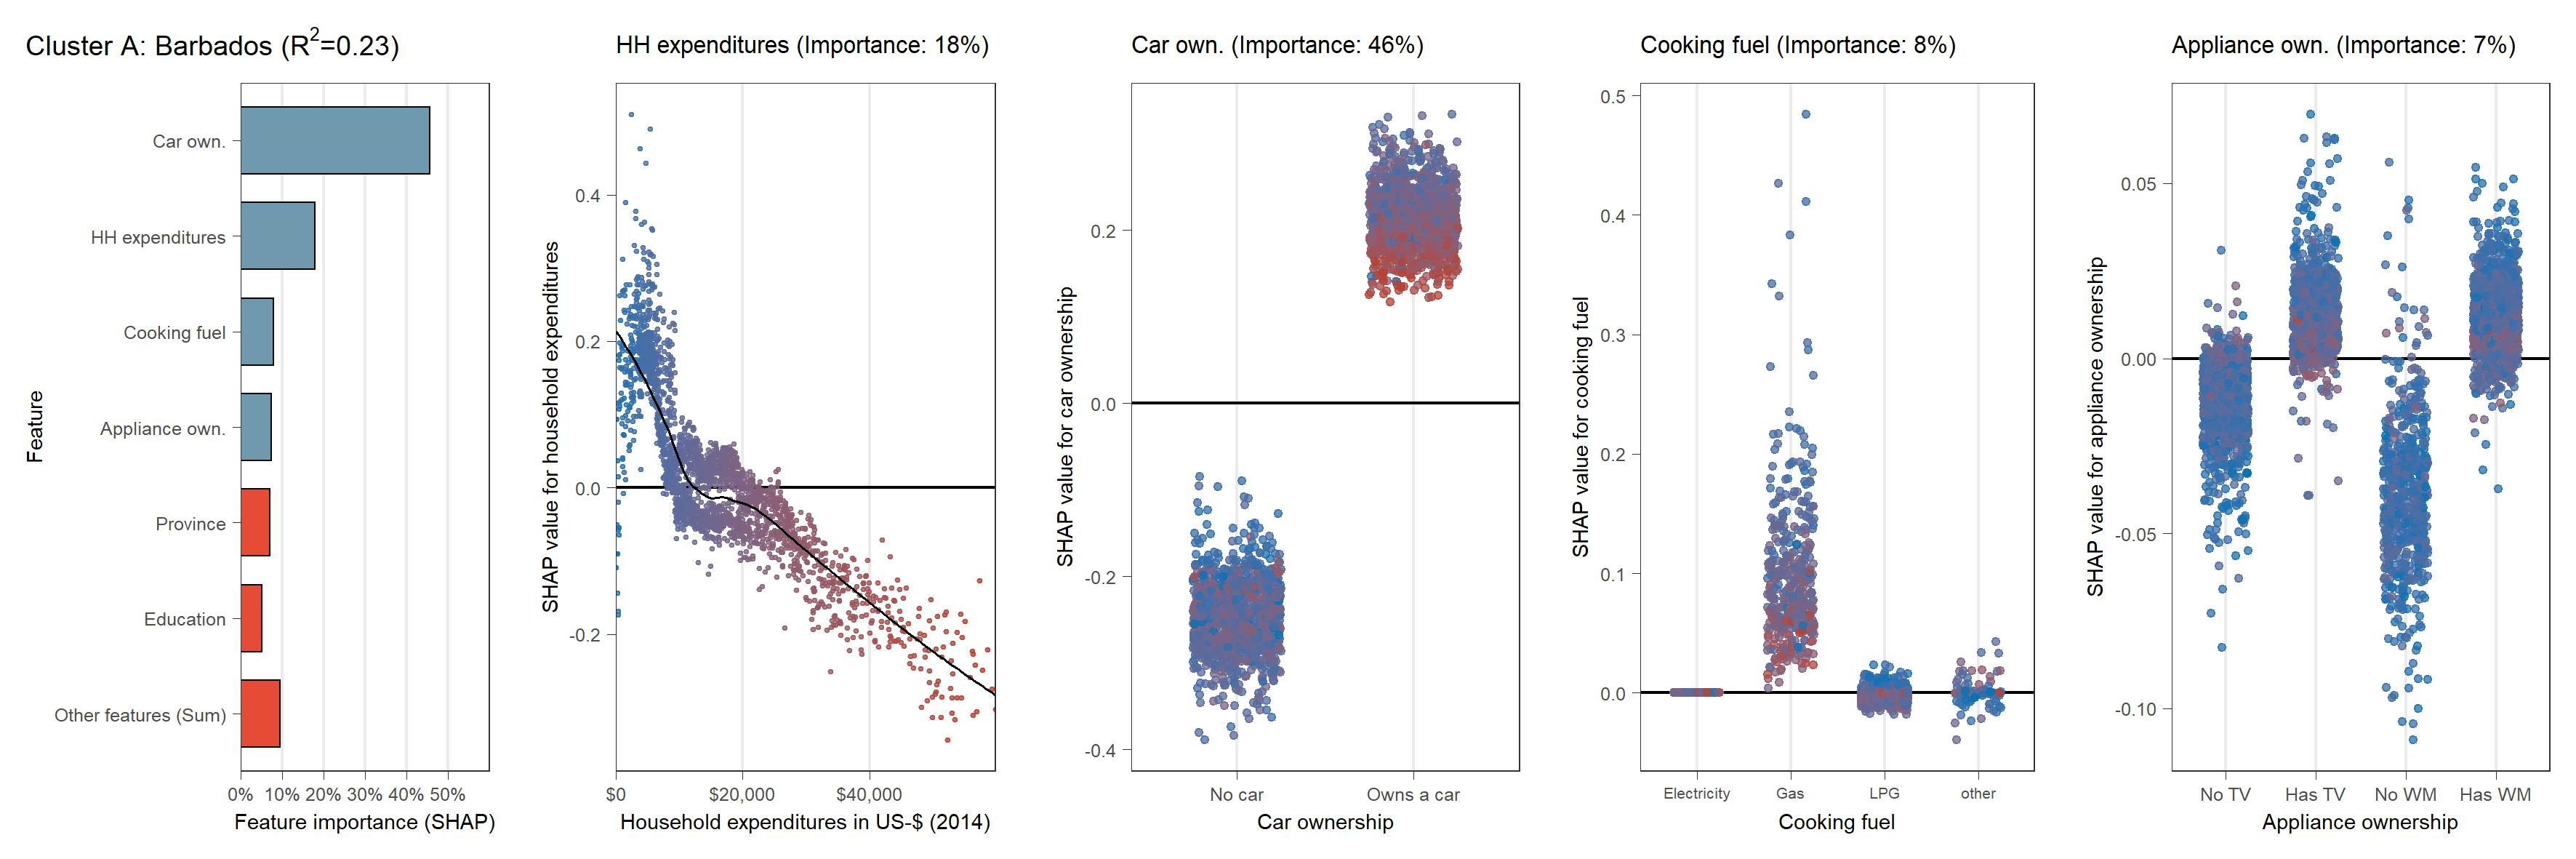
\includegraphics[width=\textwidth]{Figure 5b/Figure_5b_BRB}     \end{subfigure}
    \\
    \vspace{0.5cm}
    \begin{subcaption2}
     This figure shows SHAP-values for predicting carbon intensity over feature values for 87 countries in order of nine country-clusters and silhouette width. The bar chart displays normalized average absolute SHAP-values for all features. Features with less than 3\% of normalized SHAP-values are subsumed as "Other features (Sum)". Charts show SHAP-values over total household expenditures for all countries and for the three most important features in each country besides total household expenditures. Colors represent household expenditures with blue (red) colors indicating lower (higher) household expenditures.
     \end{subcaption2}
\end{figure}

\begin{figure}[ht!]\ContinuedFloat
    \centering
   \begin{subfigure}[b]{\textwidth}
         \centering
         \caption{Partial dependence plot (SHAP) for Canada (cluster A)}
         \label{fig:5b_CAN}
         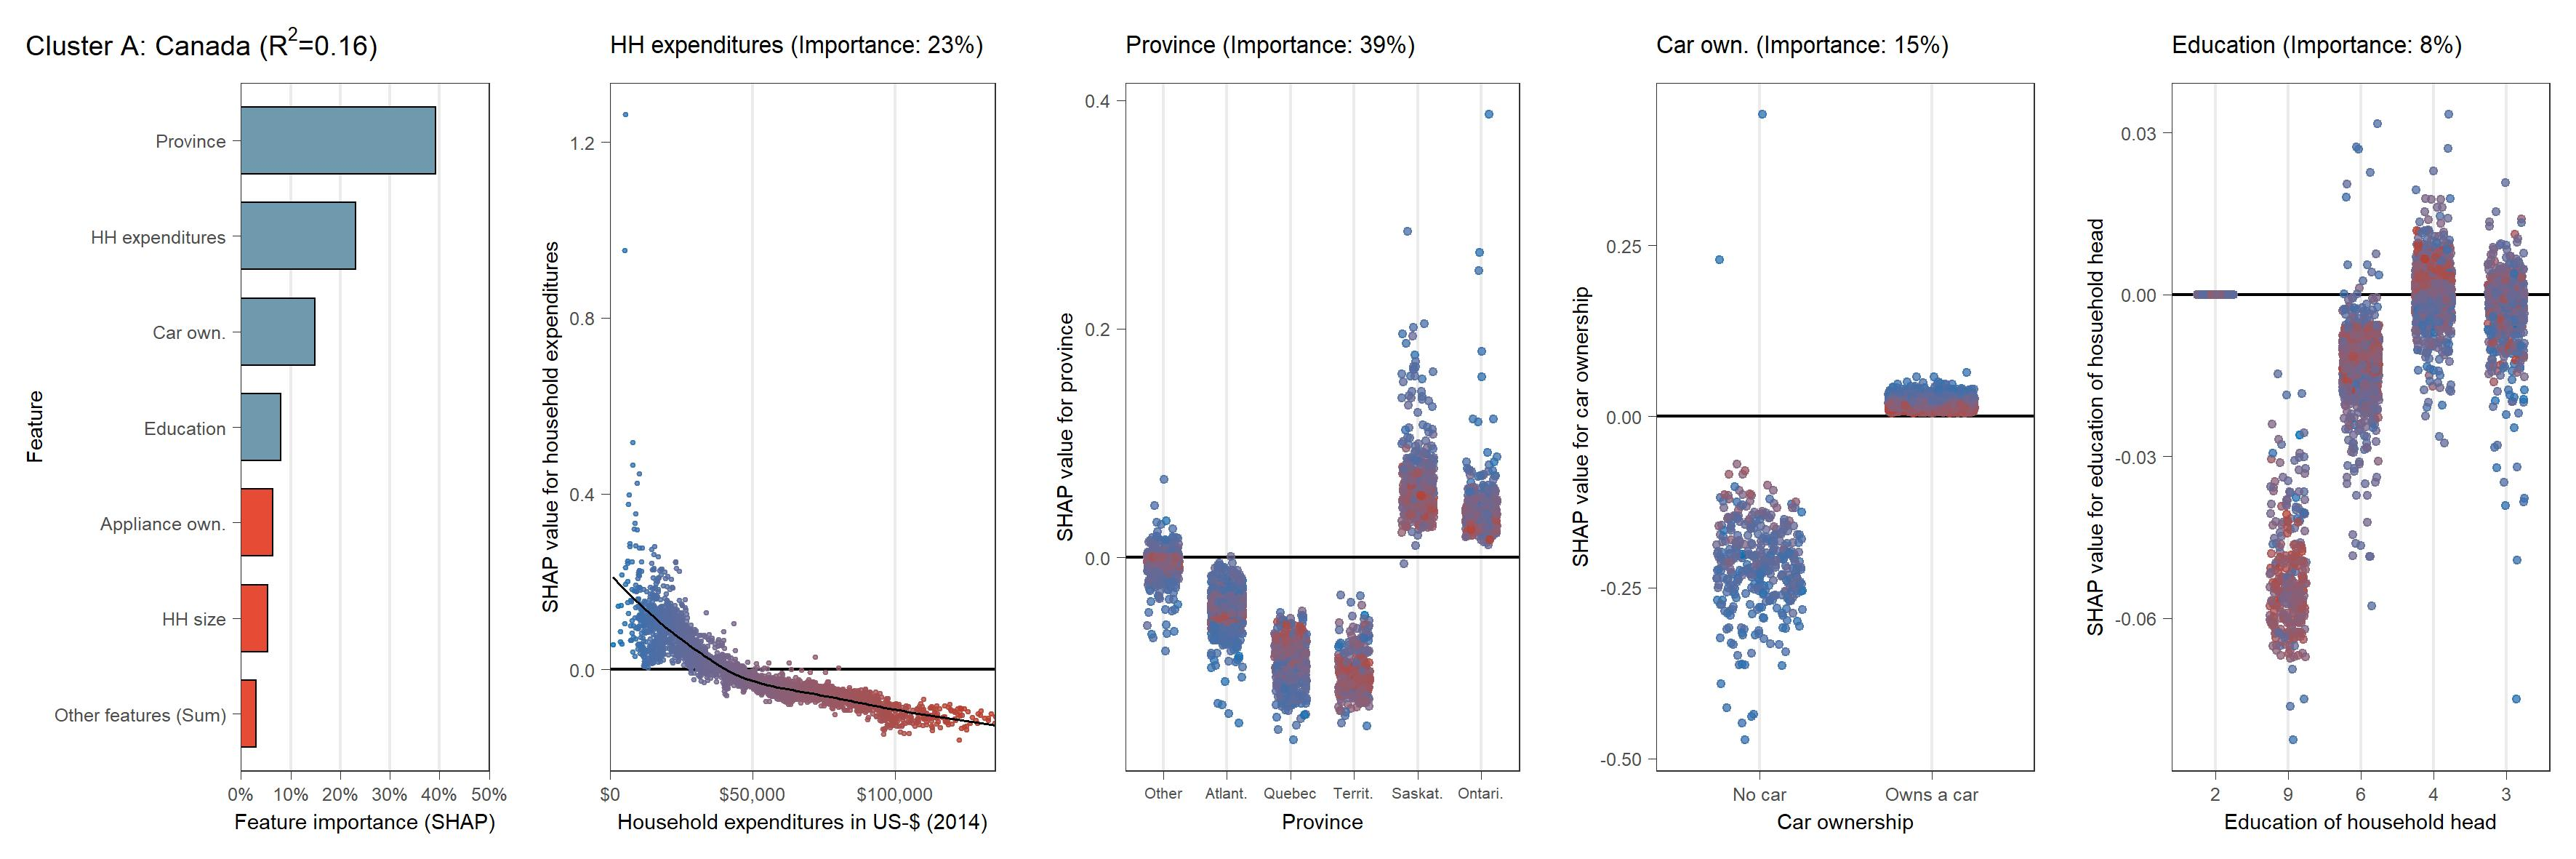
\includegraphics[width=\textwidth]{Figure 5b/Figure_5b_CAN}
         \end{subfigure}
    \\
    \vspace{0.5cm}
   \begin{subfigure}[b]{\textwidth}
         \centering
         \caption{Partial dependence plot (SHAP) for Switzerland (cluster A)}
         \label{fig:5b_CHE}
         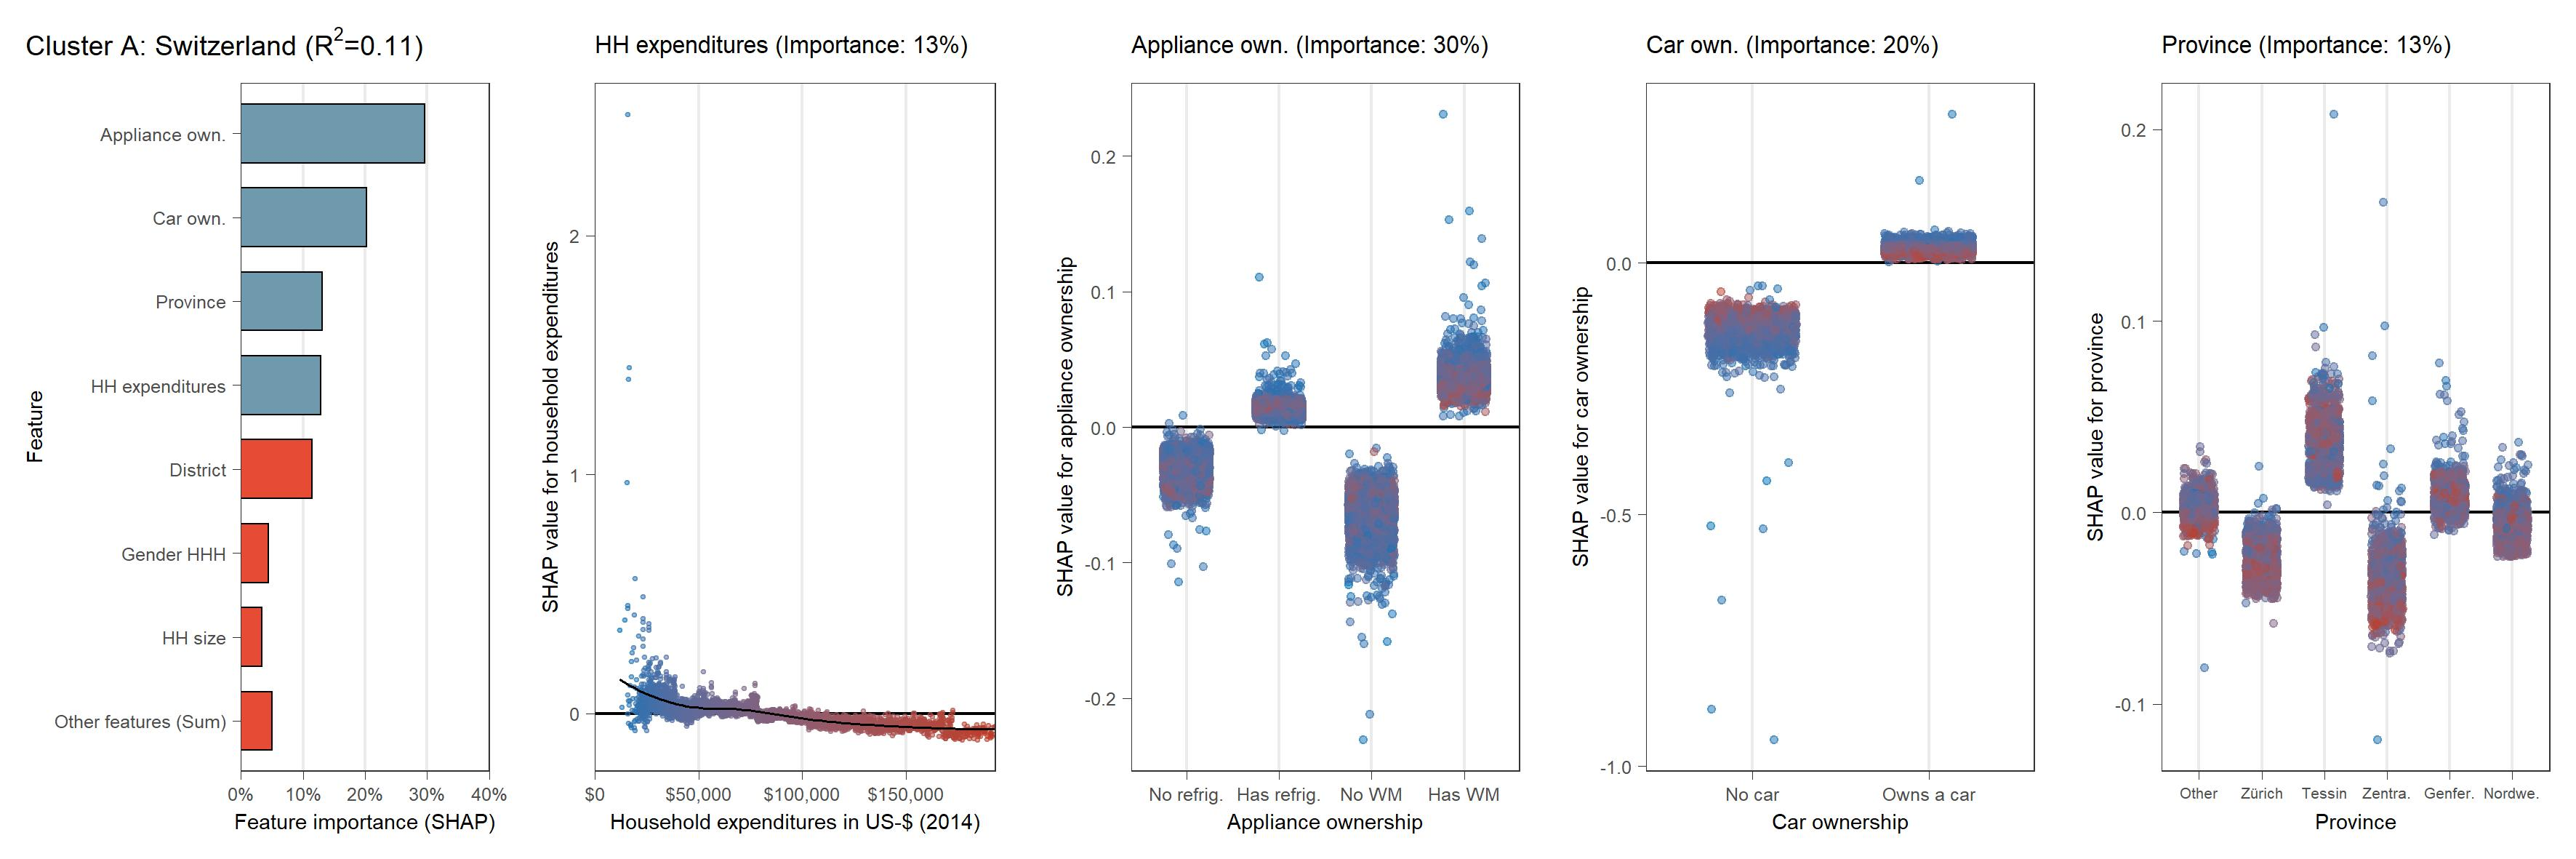
\includegraphics[width=\textwidth]{Figure 5b/Figure_5b_CHE}
         \end{subfigure}
    \\
    \vspace{0.5cm}
   \begin{subfigure}[b]{\textwidth}
         \centering
         \caption{Partial dependence plot (SHAP) for Chile (cluster A)}
         \label{fig:5b_CHL}
         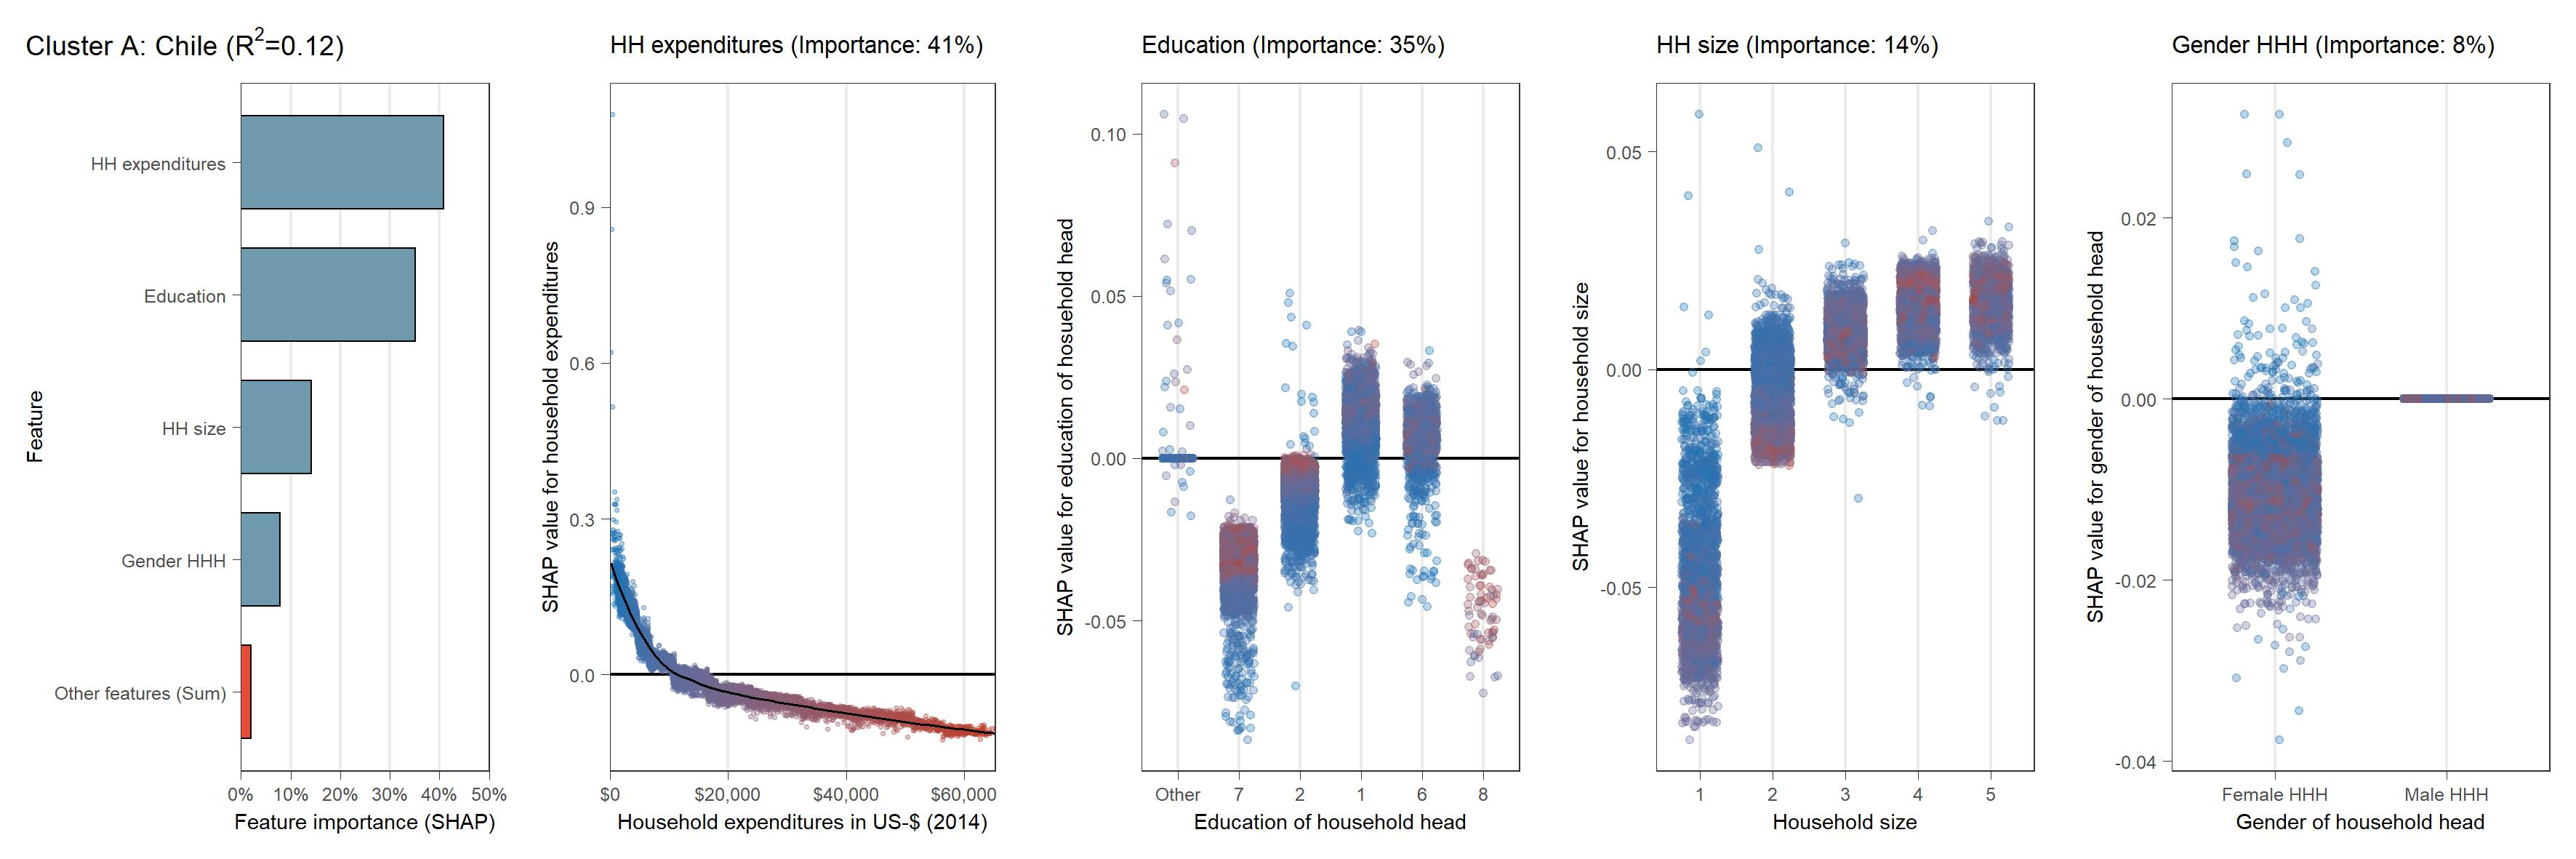
\includegraphics[width=\textwidth]{Figure 5b/Figure_5b_CHL}
    \end{subfigure}
    \\
    \vspace{0.5cm}
    \begin{subcaption2}
     This figure shows SHAP-values for predicting carbon intensity over feature values for 87 countries in order of nine country-clusters and silhouette width. The bar chart displays normalized average absolute SHAP-values for all features. Features with less than 3\% of normalized SHAP-values are subsumed as "Other features (Sum)". Charts show SHAP-values over total household expenditures for all countries and for the three most important features in each country besides total household expenditures. Colors represent household expenditures with blue (red) colors indicating lower (higher) household expenditures.
     \end{subcaption2}
\end{figure}

\begin{figure}[ht!]\ContinuedFloat
    \centering
   \begin{subfigure}[b]{\textwidth}
         \centering
         \caption{Partial dependence plot (SHAP) for Colombia (cluster A)}
         \label{fig:5b_COL}
         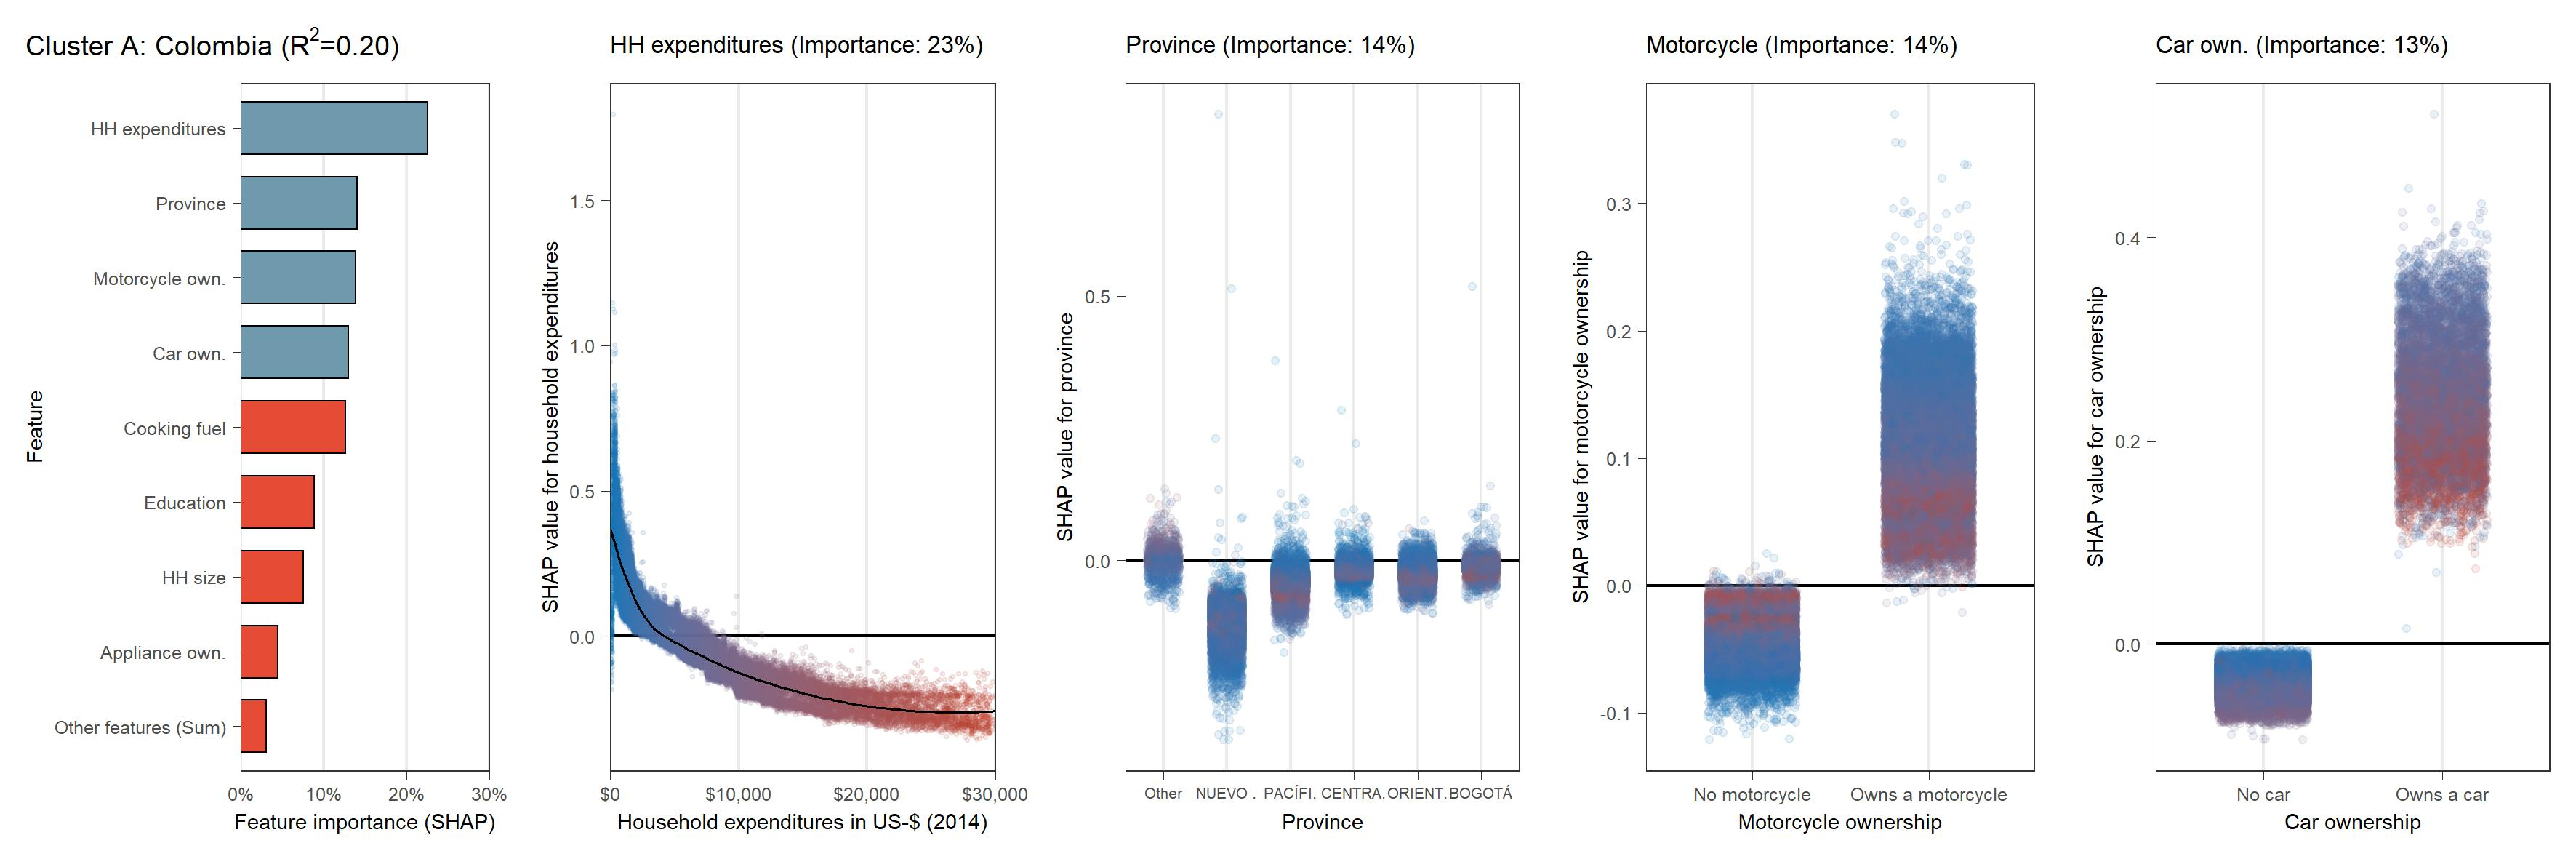
\includegraphics[width=\textwidth]{Figure 5b/Figure_5b_COL}
         \end{subfigure}
    \\
    \vspace{0.5cm}
   \begin{subfigure}[b]{\textwidth}
      \centering
      \caption{Partial dependence plot (SHAP) for Costa Rica (cluster A)}
      \label{fig:5b_CRI}
      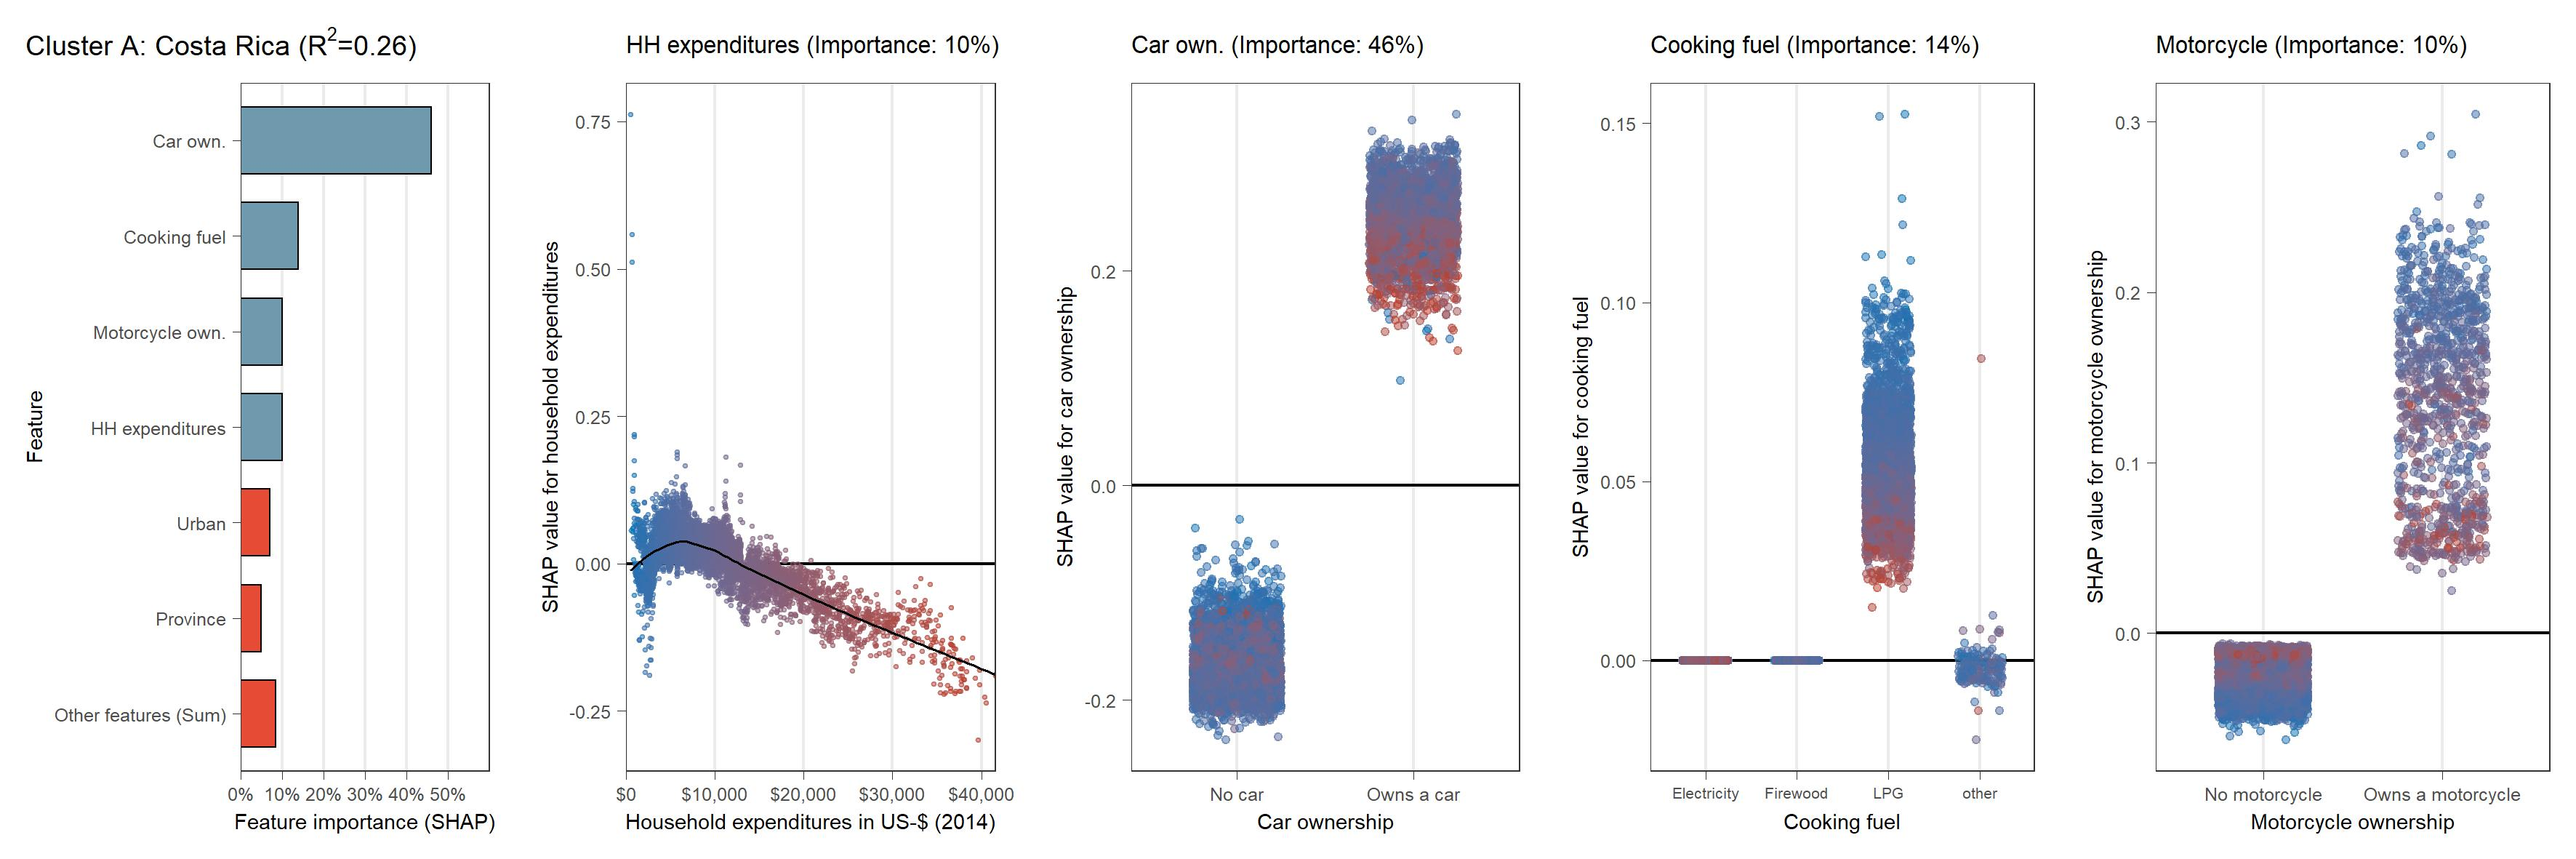
\includegraphics[width=\textwidth]{Figure 5b/Figure_5b_CRI}       
     \end{subfigure}
    \\
    \vspace{0.5cm}
   \begin{subfigure}[b]{\textwidth}
         \centering
         \caption{Partial dependence plot (SHAP) for Cyprus (cluster A)}
         \label{fig:5b_CYP}
         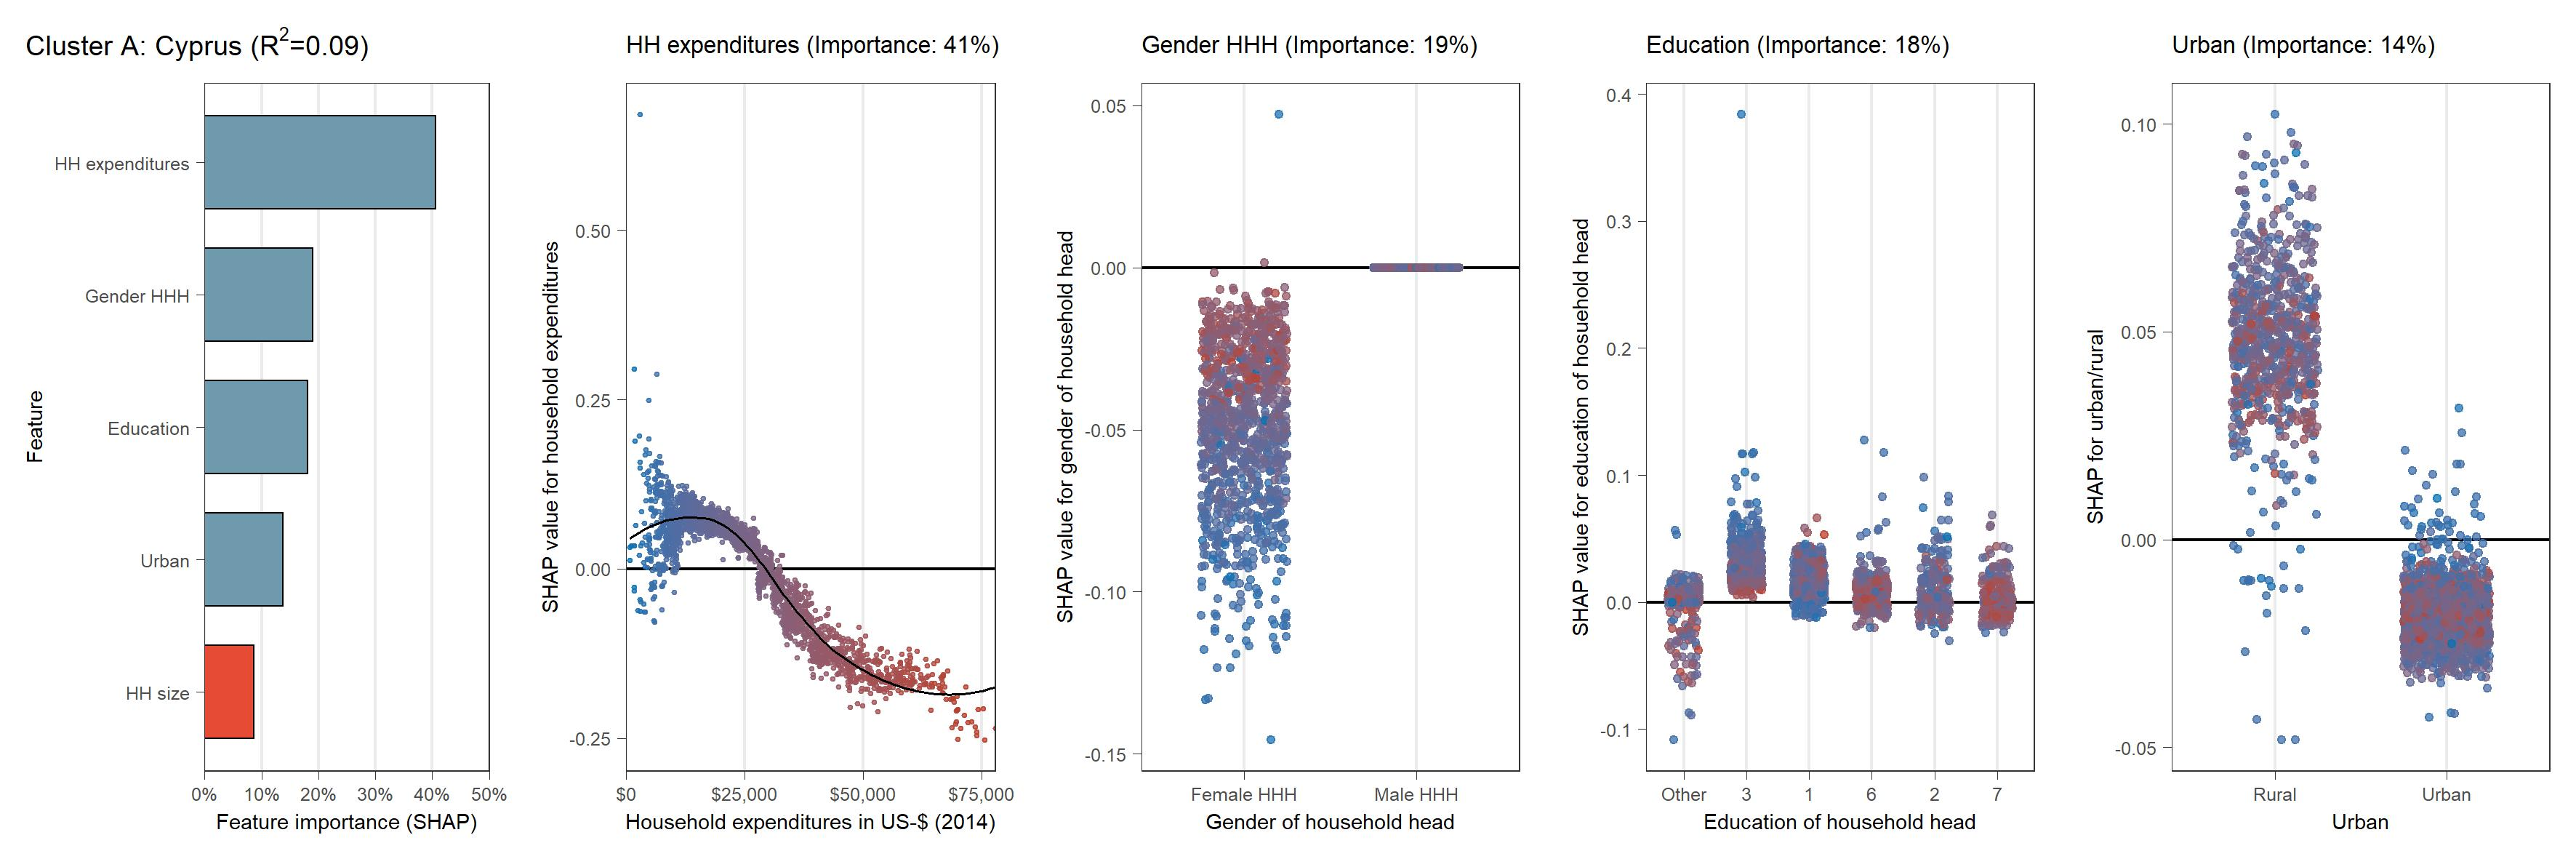
\includegraphics[width=\textwidth]{Figure 5b/Figure_5b_CYP}
         \end{subfigure}
    \\
    \vspace{0.5cm}
    \begin{subcaption2}
     This figure shows SHAP-values for predicting carbon intensity over feature values for 87 countries in order of nine country-clusters and silhouette width. The bar chart displays normalized average absolute SHAP-values for all features. Features with less than 3\% of normalized SHAP-values are subsumed as "Other features (Sum)". Charts show SHAP-values over total household expenditures for all countries and for the three most important features in each country besides total household expenditures. Colors represent household expenditures with blue (red) colors indicating lower (higher) household expenditures.
     \end{subcaption2}
\end{figure}

\begin{figure}[ht!]\ContinuedFloat
    \centering
   \begin{subfigure}[b]{\textwidth}
          \centering
         \caption{Partial dependence plot (SHAP) for Czech Republic (cluster A)}
         \label{fig:5b_CZE}
         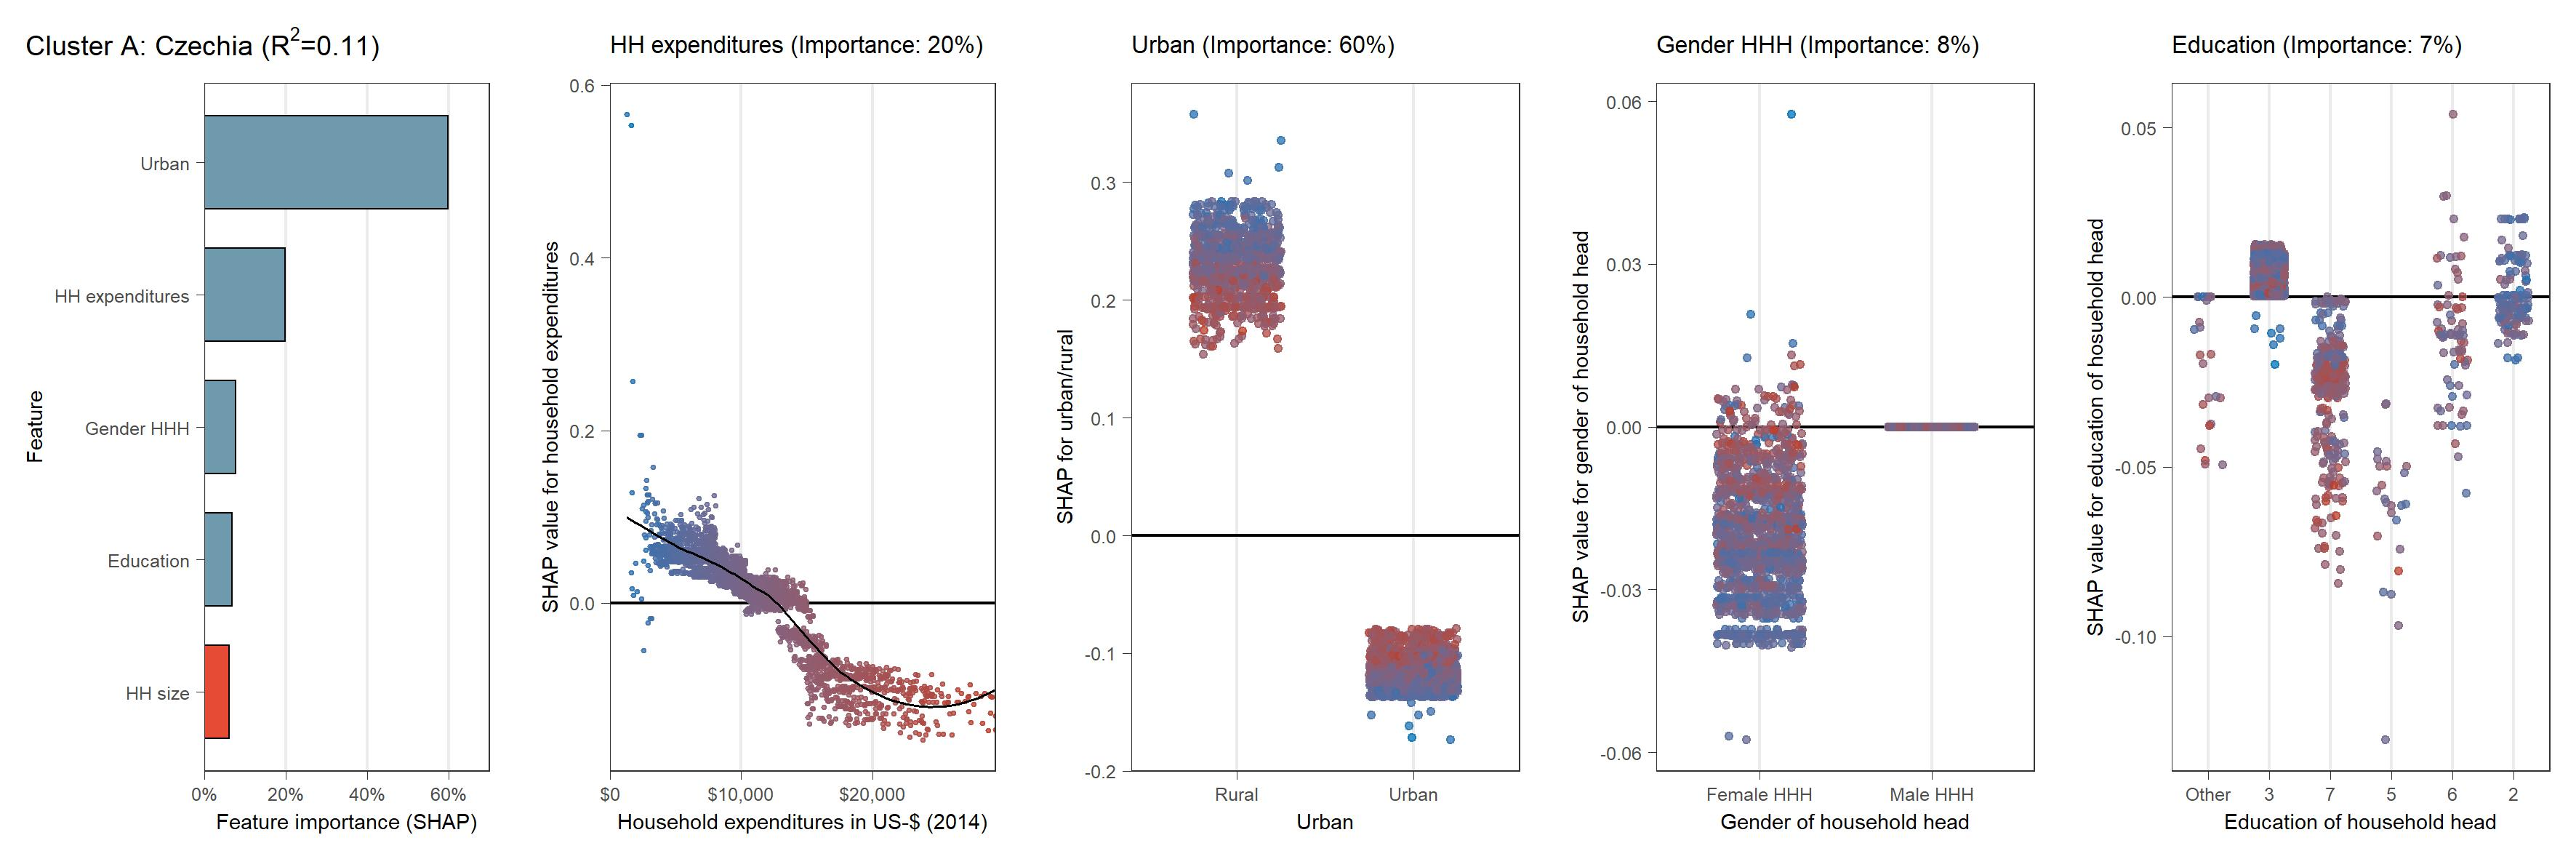
\includegraphics[width=\textwidth]{Figure 5b/Figure_5b_CZE}    \end{subfigure}
    \\
    \vspace{0.5cm}
   \begin{subfigure}[b]{\textwidth}
         \centering
         \caption{Partial dependence plot (SHAP) for Germany (cluster A)}
         \label{fig:5b_DEU}
         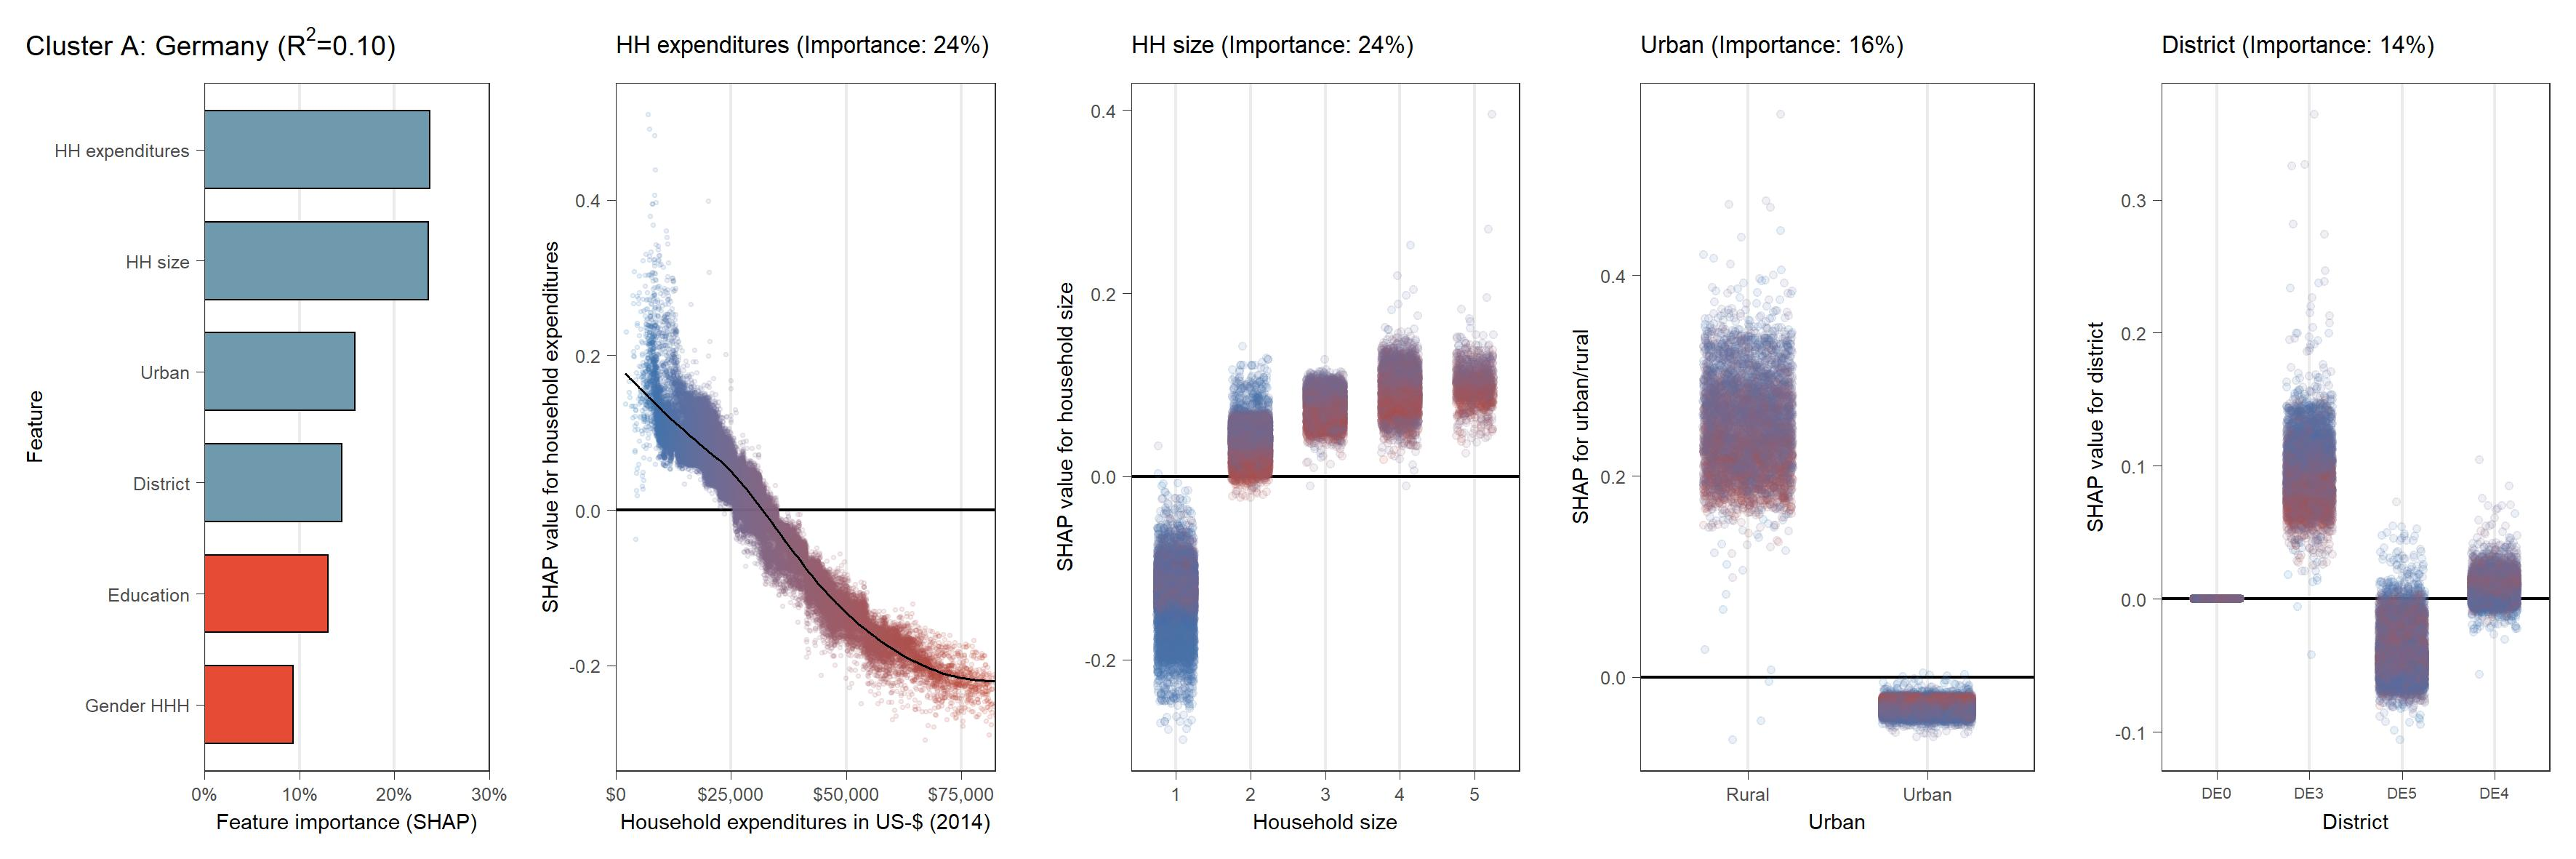
\includegraphics[width=\textwidth]{Figure 5b/Figure_5b_DEU}
         \end{subfigure}
    \\
    \vspace{0.5cm}
   \begin{subfigure}[b]{\textwidth}
         \centering
         \caption{Partial dependence plot (SHAP) for Denmark (cluster A)}
         \label{fig:5b_DNK}
         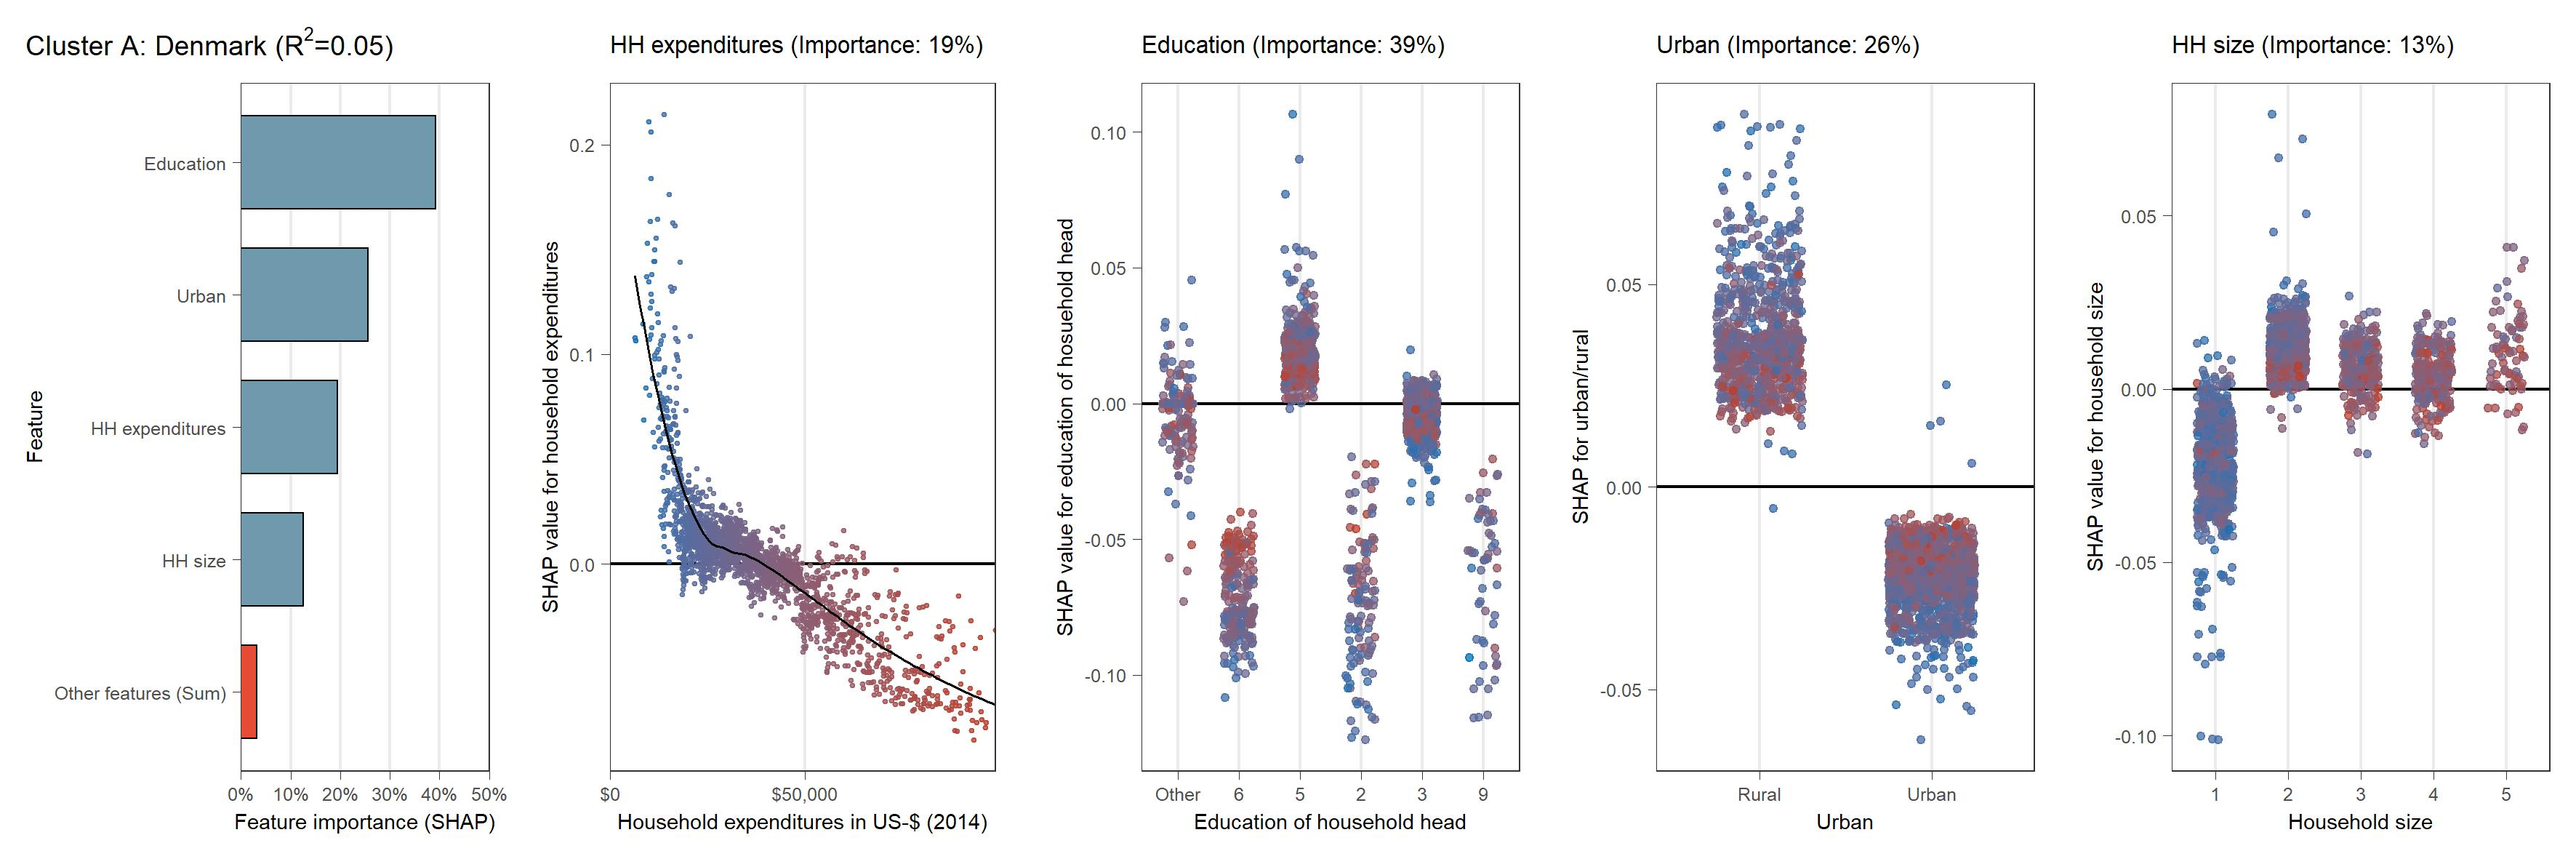
\includegraphics[width=\textwidth]{Figure 5b/Figure_5b_DNK} \end{subfigure}
    \\
    \vspace{0.5cm}
    \begin{subcaption2}
     This figure shows SHAP-values for predicting carbon intensity over feature values for 87 countries in order of nine country-clusters and silhouette width. The bar chart displays normalized average absolute SHAP-values for all features. Features with less than 3\% of normalized SHAP-values are subsumed as "Other features (Sum)". Charts show SHAP-values over total household expenditures for all countries and for the three most important features in each country besides total household expenditures. Colors represent household expenditures with blue (red) colors indicating lower (higher) household expenditures.
     \end{subcaption2}
\end{figure}

\begin{figure}[ht!]\ContinuedFloat
    \centering
   \begin{subfigure}[b]{\textwidth}
          \centering
         \caption{Partial dependence plot (SHAP) for Spain (cluster A)}
         \label{fig:5b_ESP}
         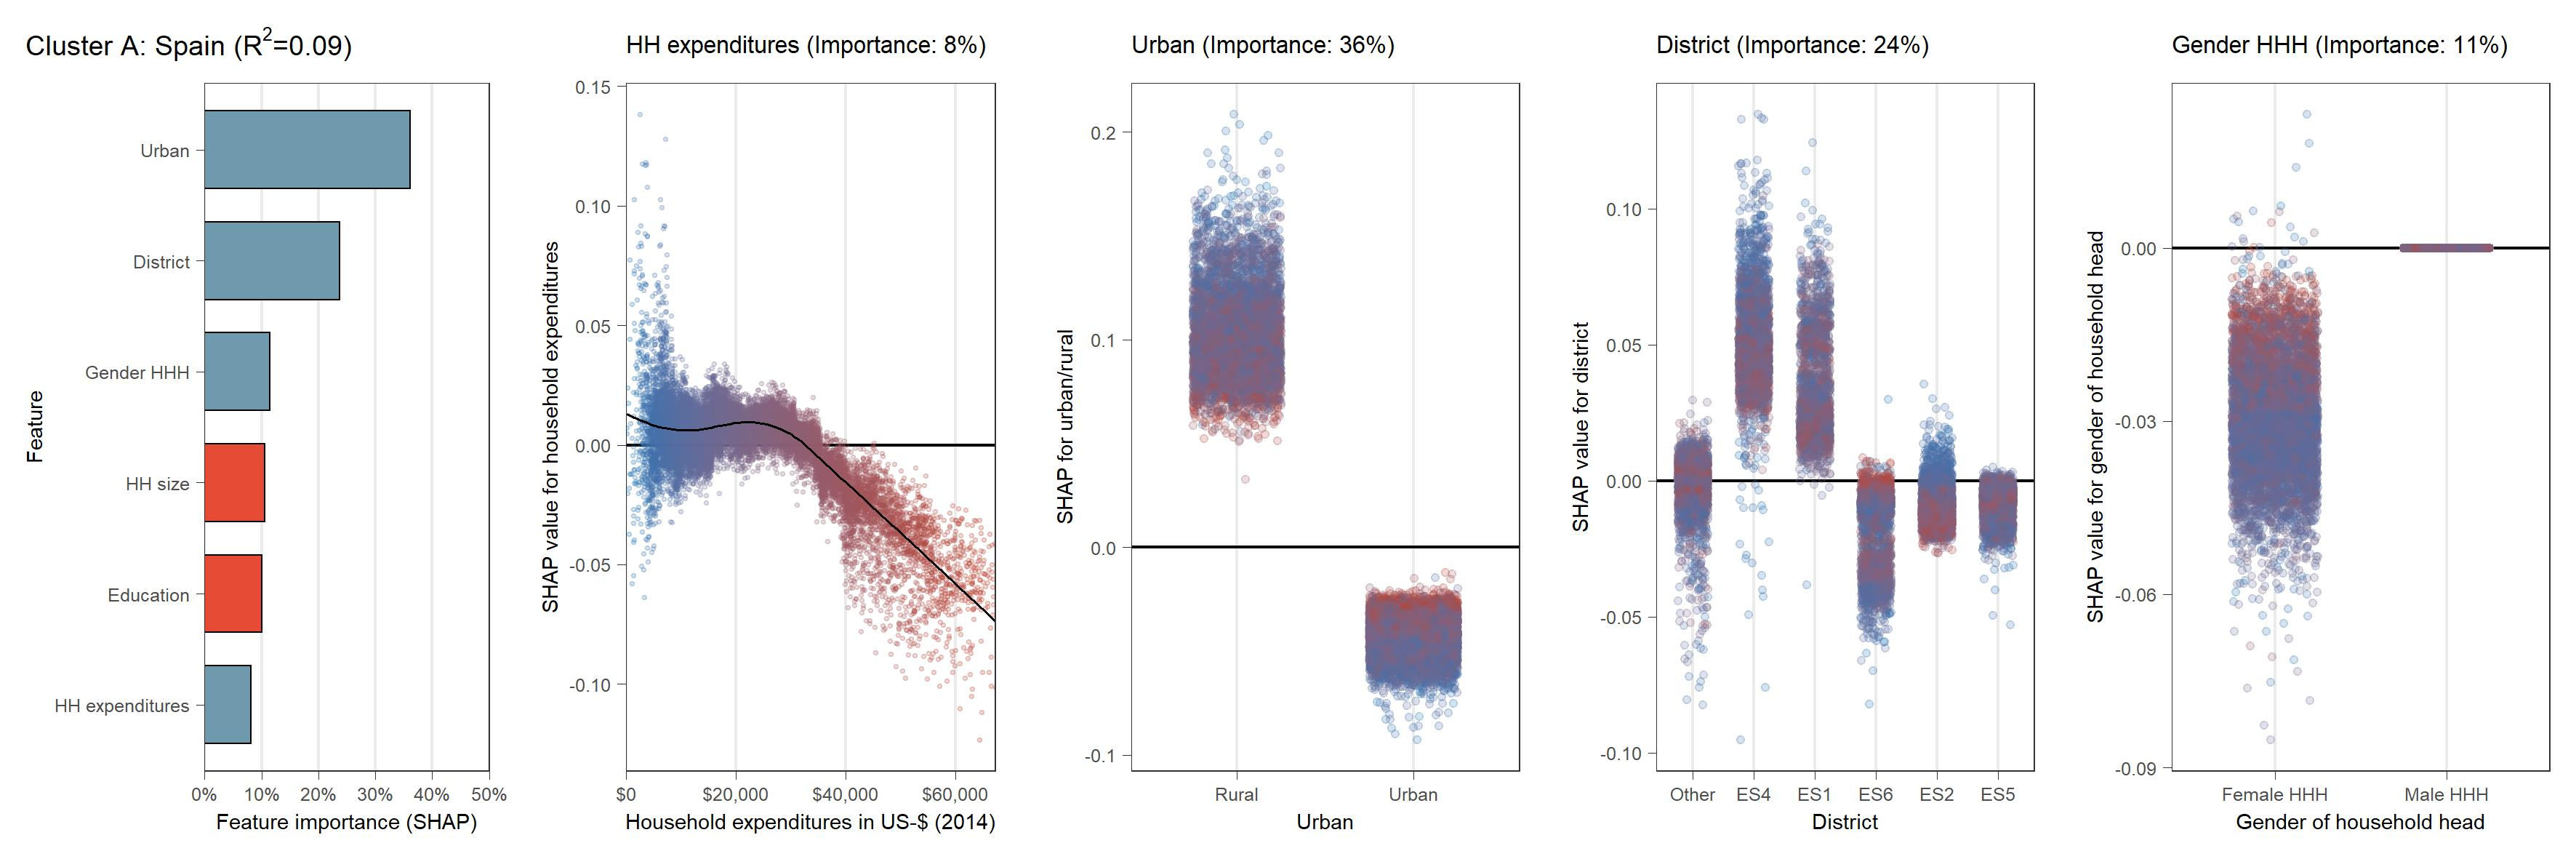
\includegraphics[width=\textwidth]{Figure 5b/Figure_5b_ESP}
     \end{subfigure}
    \\
    \vspace{0.5cm}
   \begin{subfigure}[b]{\textwidth}   
         \centering
         \caption{Partial dependence plot (SHAP) for Estonia (cluster A)}
         \label{fig:5b_EST}
         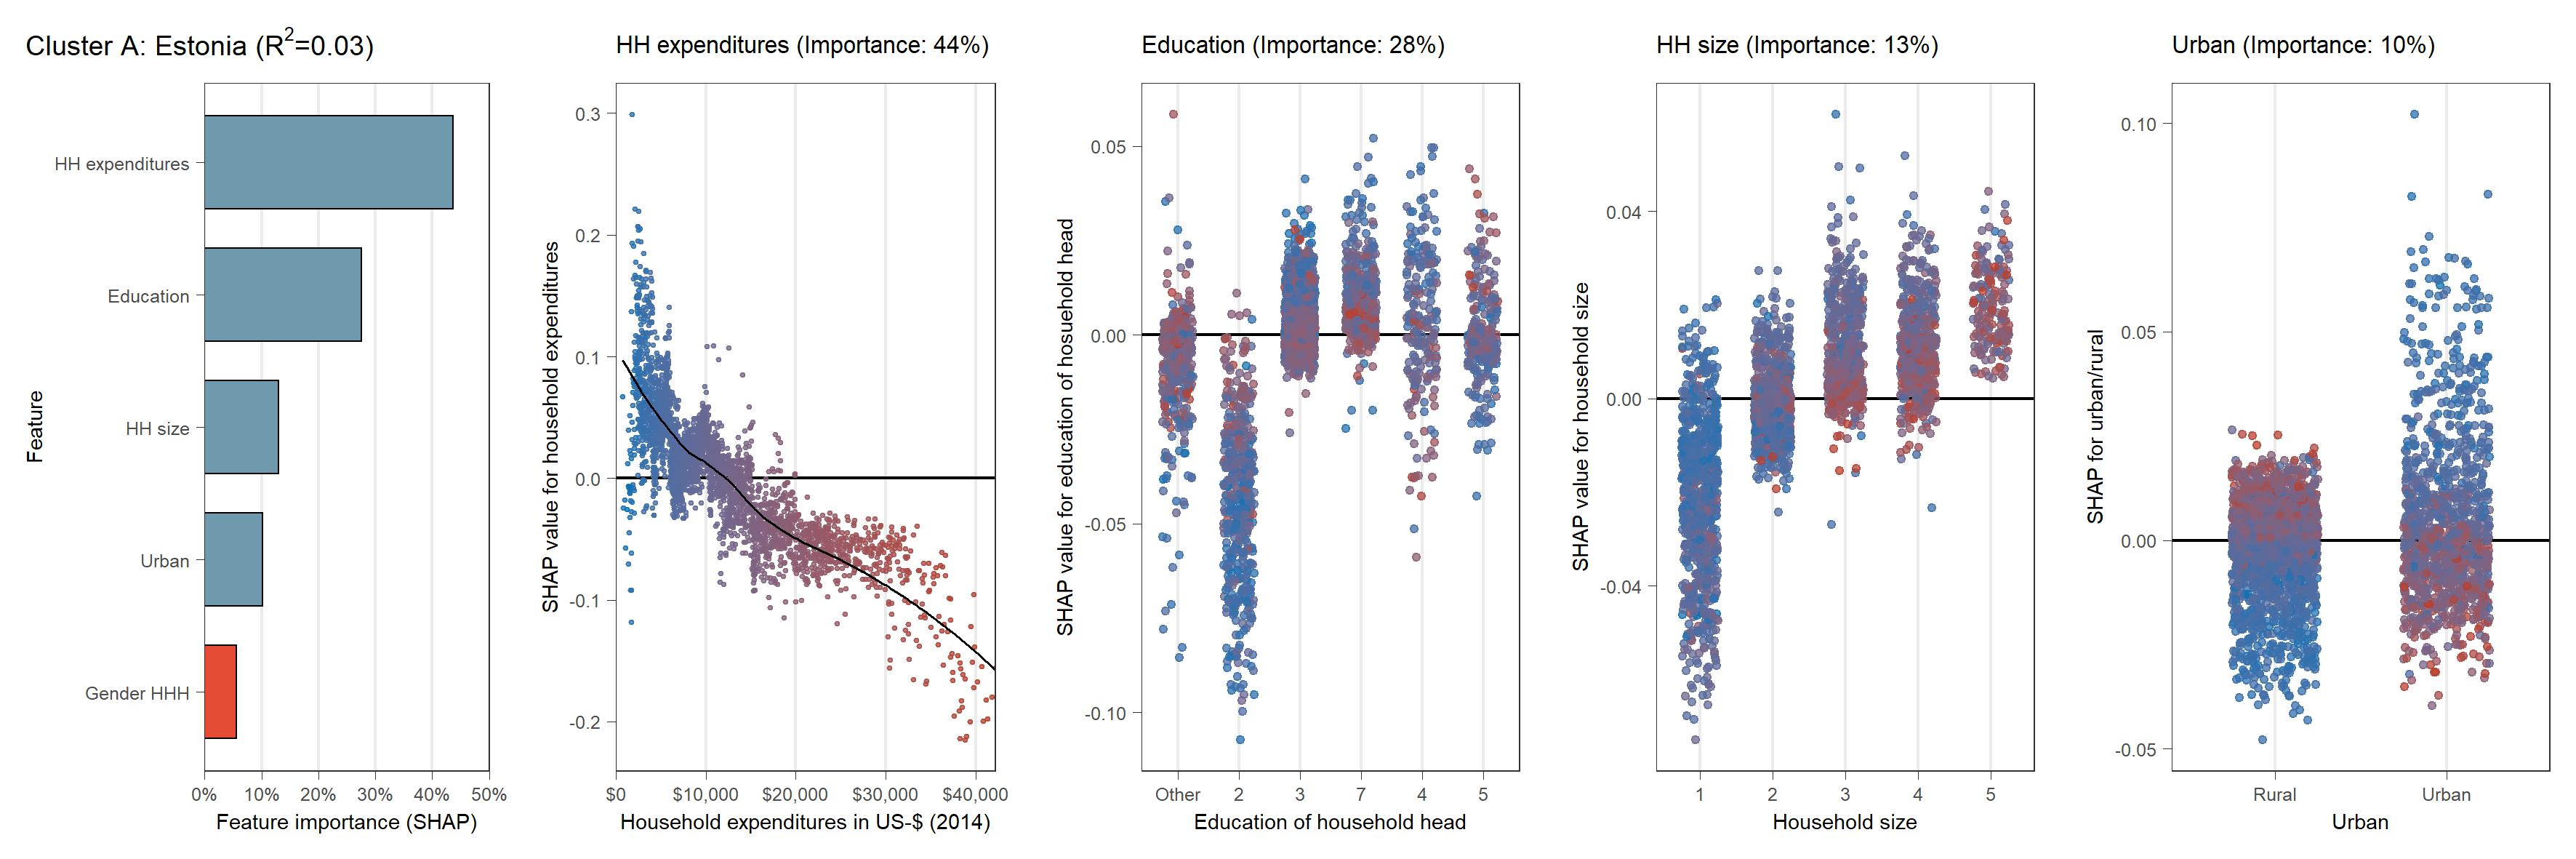
\includegraphics[width=\textwidth]{Figure 5b/Figure_5b_EST}
         \end{subfigure}
    \\
    \vspace{0.5cm}
   \begin{subfigure}[b]{\textwidth}
         \centering
         \caption{Partial dependence plot (SHAP) for Ethiopia (cluster A)}
         \label{fig:5b_ETH}
         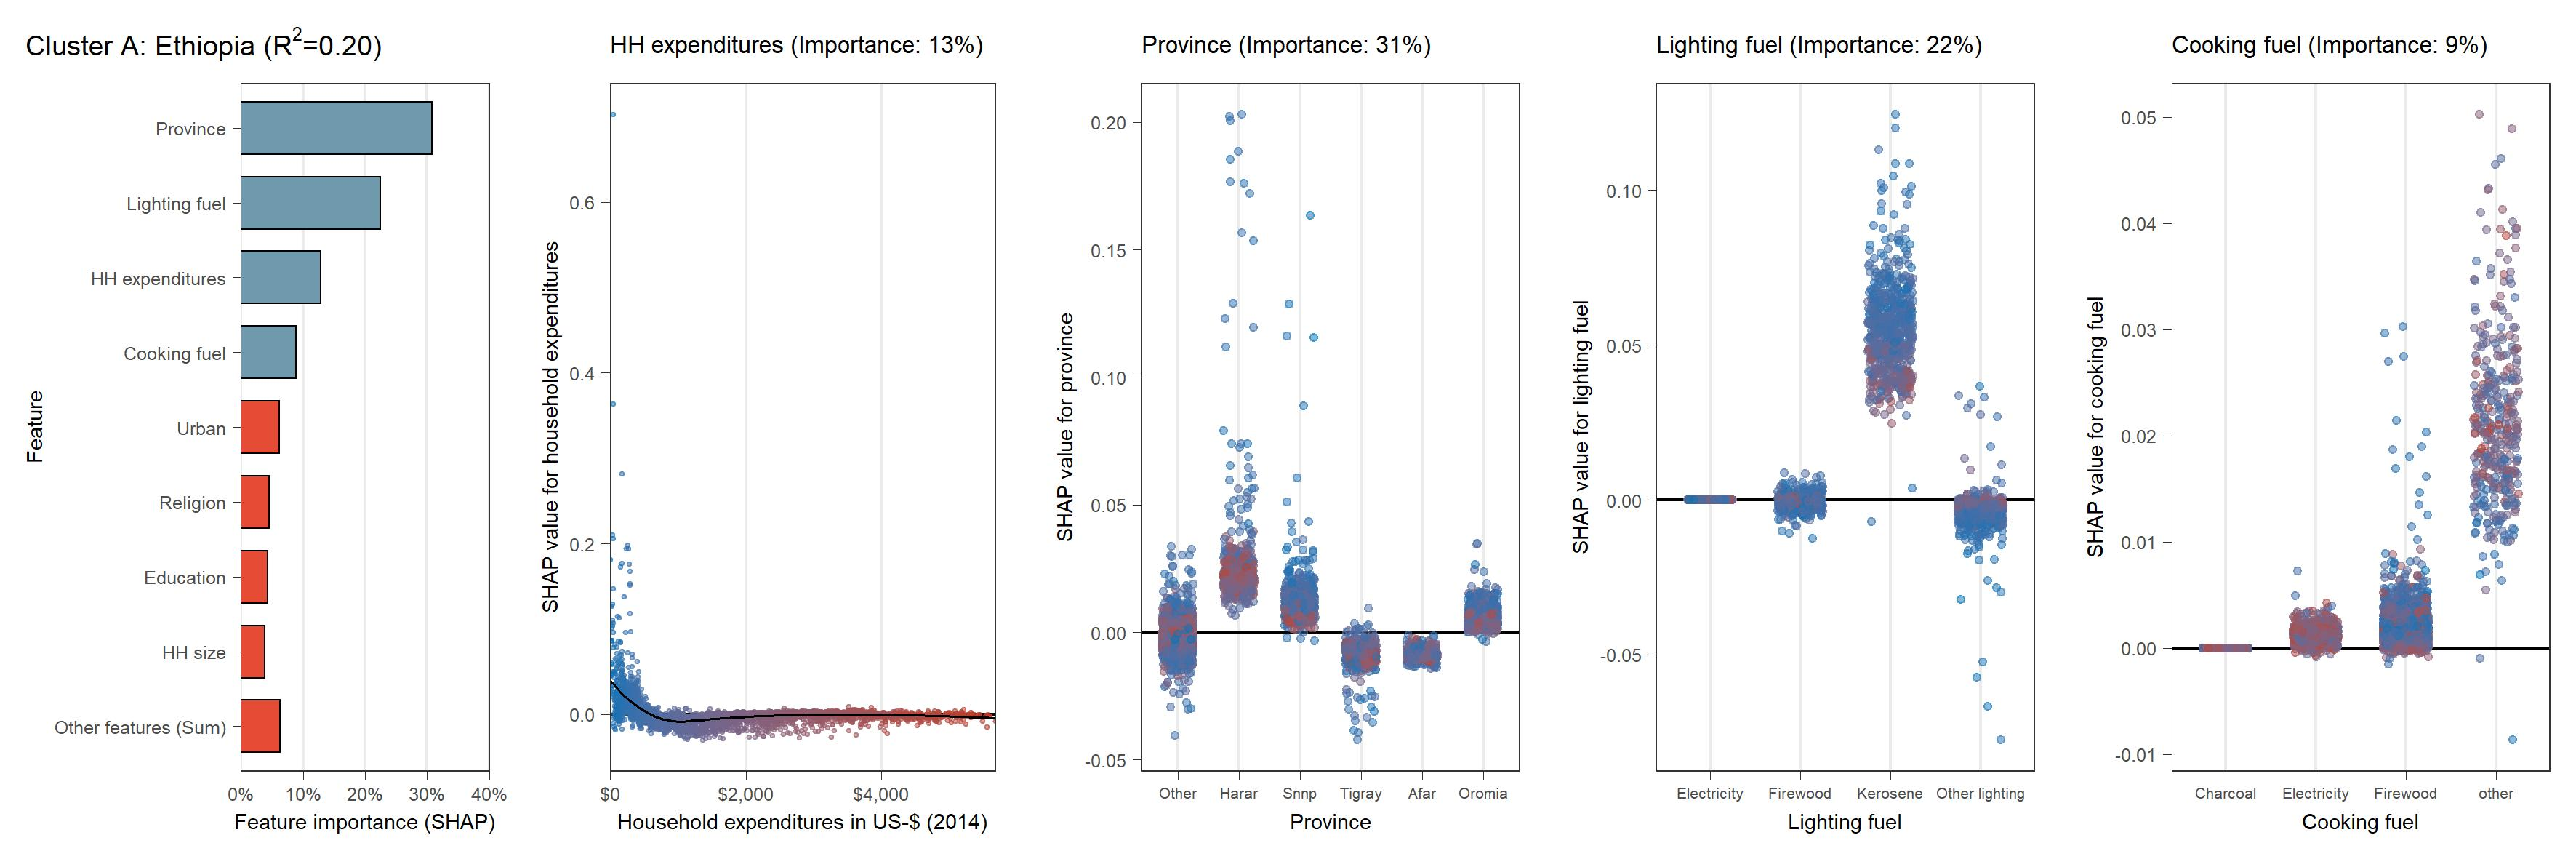
\includegraphics[width=\textwidth]{Figure 5b/Figure_5b_ETH} \end{subfigure}
    \\
    \vspace{0.5cm}
    \begin{subcaption2}
     This figure shows SHAP-values for predicting carbon intensity over feature values for 87 countries in order of nine country-clusters and silhouette width. The bar chart displays normalized average absolute SHAP-values for all features. Features with less than 3\% of normalized SHAP-values are subsumed as "Other features (Sum)". Charts show SHAP-values over total household expenditures for all countries and for the three most important features in each country besides total household expenditures. Colors represent household expenditures with blue (red) colors indicating lower (higher) household expenditures.
     \end{subcaption2}
\end{figure}

\begin{figure}[ht!]\ContinuedFloat
    \centering
   \begin{subfigure}[b]{\textwidth}
         \centering
         \caption{Partial dependence plot (SHAP) for Finland (cluster A)}
         \label{fig:5b_FIN}
         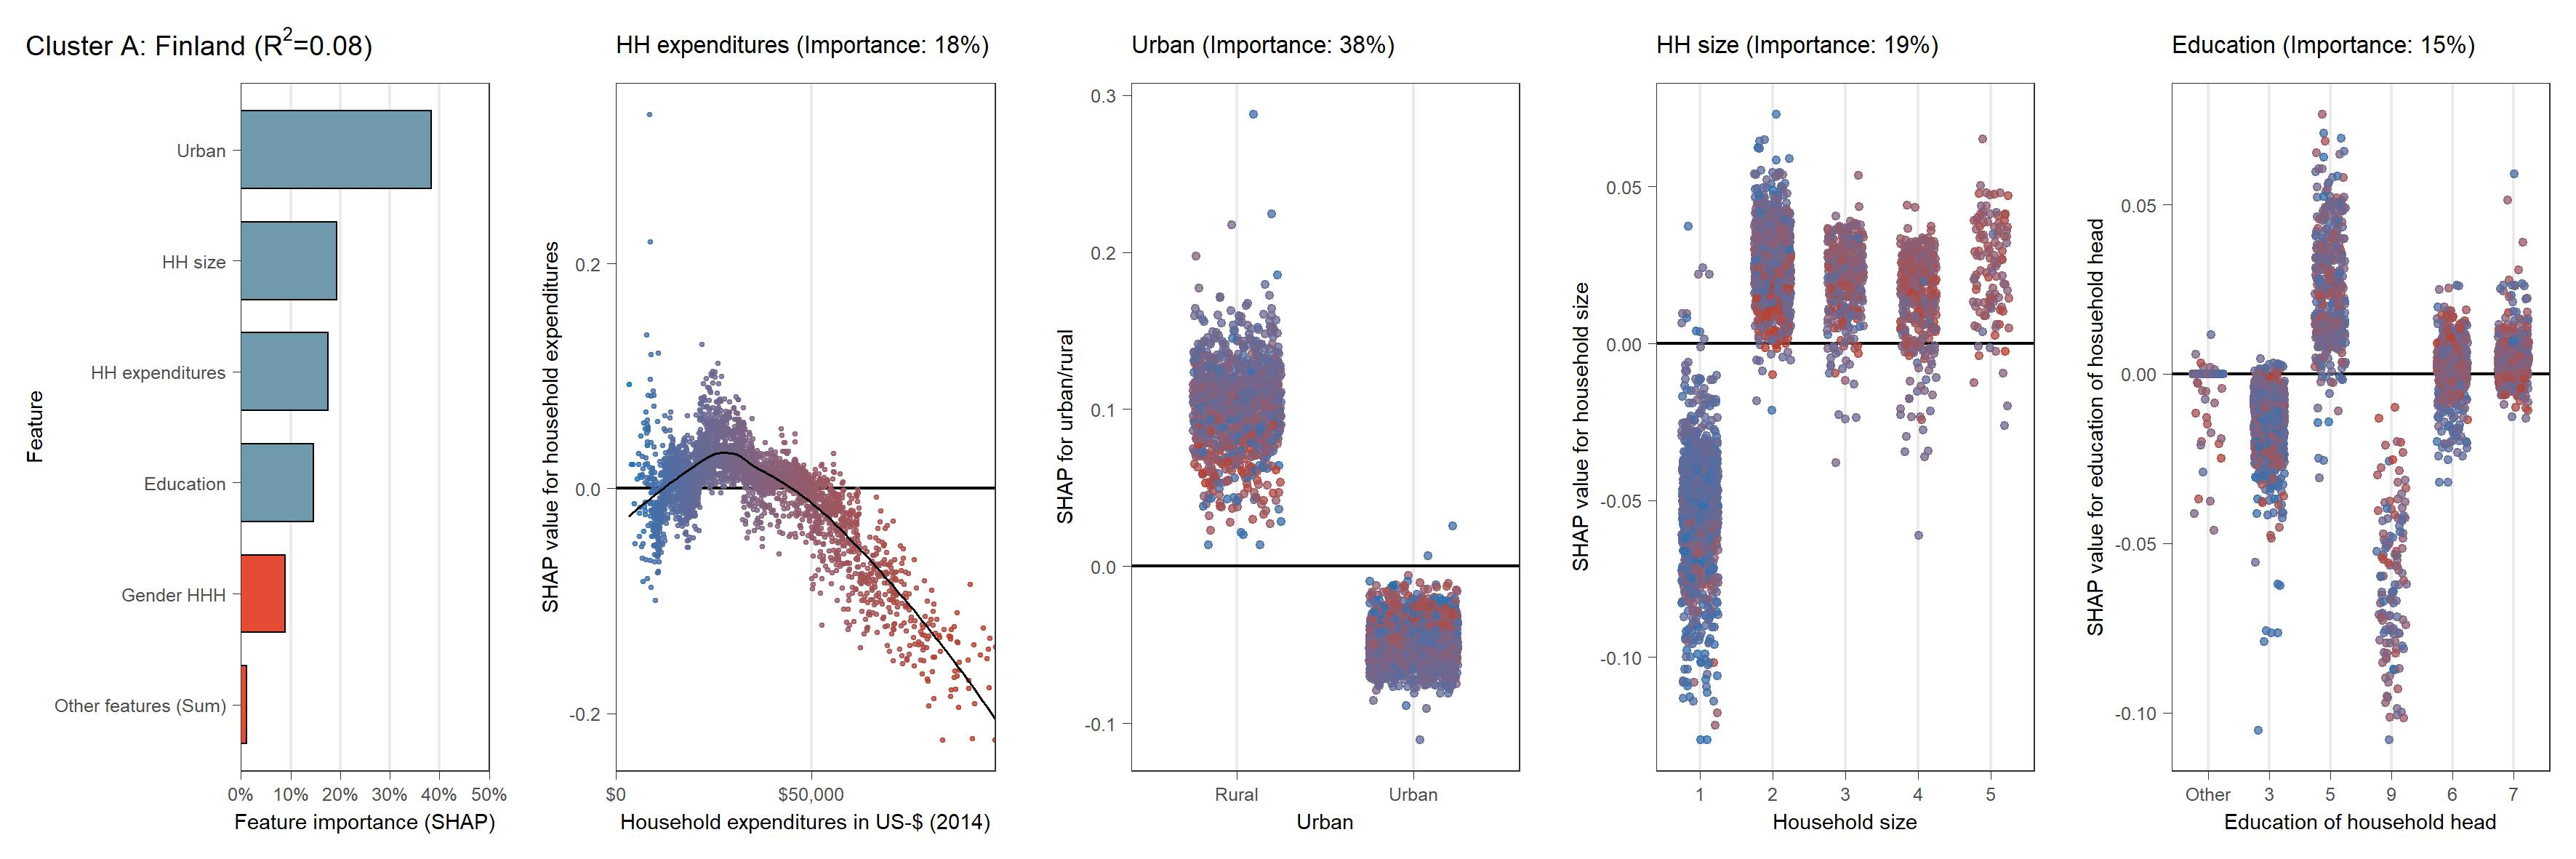
\includegraphics[width=\textwidth]{Figure 5b/Figure_5b_FIN}    
     \end{subfigure}
    \\
    \vspace{0.5cm}
   \begin{subfigure}[b]{\textwidth}
         \centering
         \caption{Partial dependence plot (SHAP) for France (cluster A)}
         \label{fig:5b_FRA}
         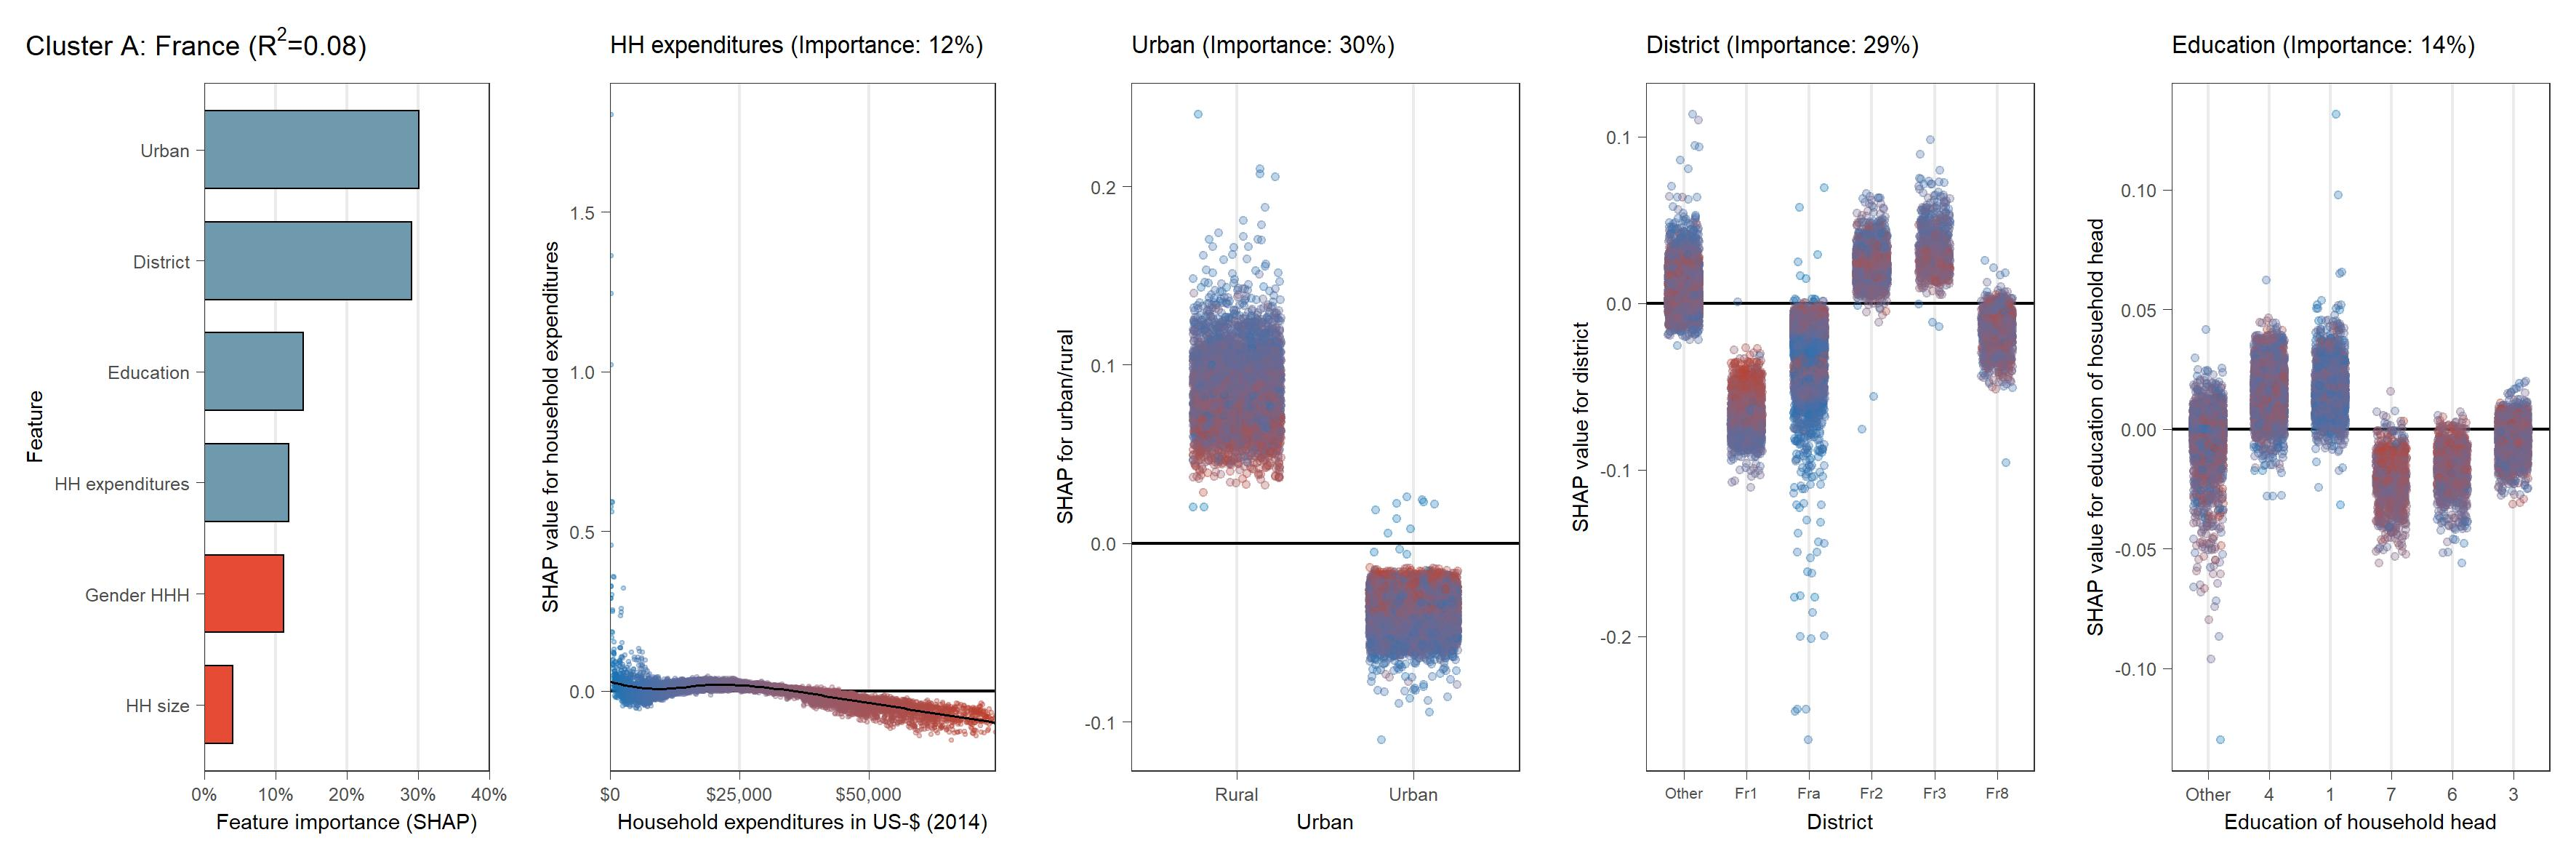
\includegraphics[width=\textwidth]{Figure 5b/Figure_5b_FRA} \end{subfigure}
    \\
    \vspace{0.5cm}
   \begin{subfigure}[b]{\textwidth}
         \centering
         \caption{Partial dependence plot (SHAP) for United Kingdom (cluster A)}
         \label{fig:5b_GBR}
         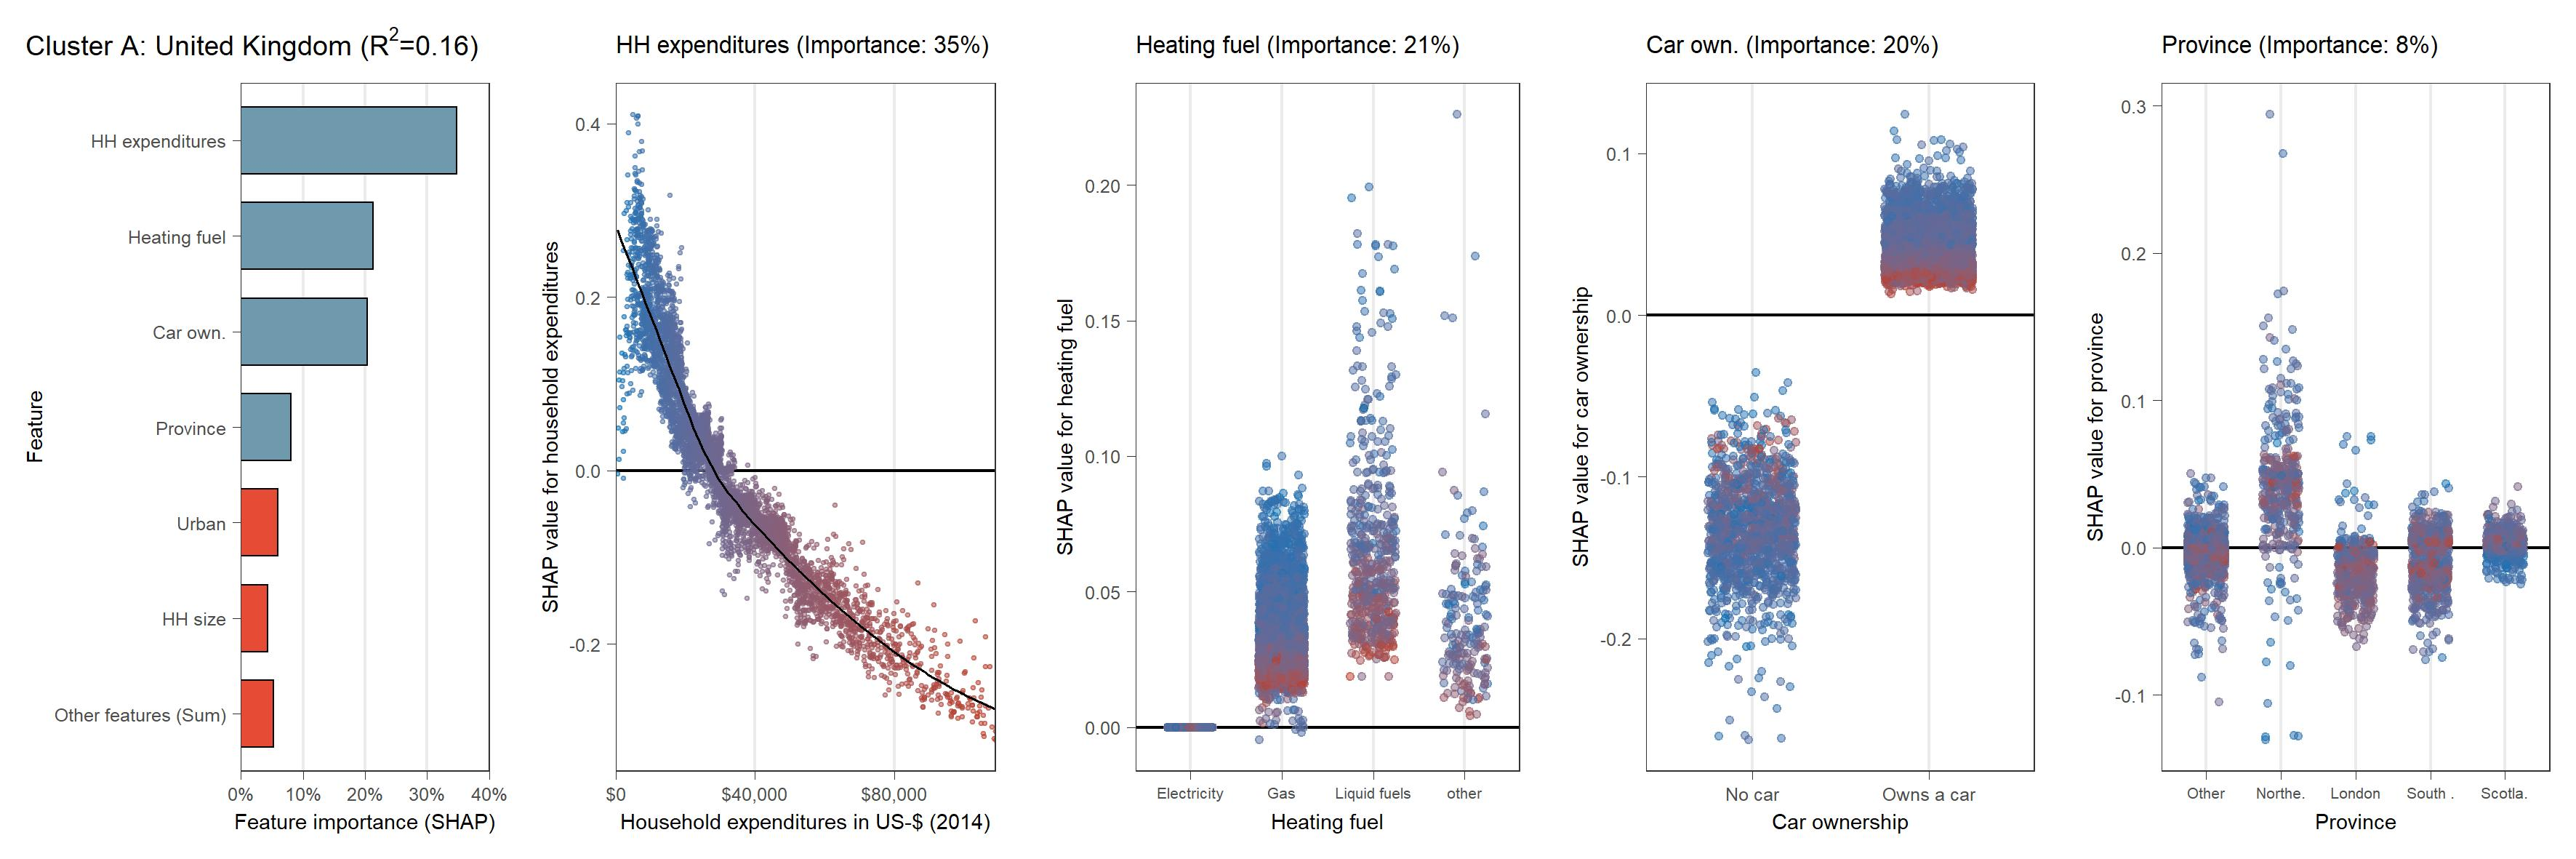
\includegraphics[width=\textwidth]{Figure 5b/Figure_5b_GBR}
    \end{subfigure}
    \\
    \vspace{0.5cm}
    \begin{subcaption2}
     This figure shows SHAP-values for predicting carbon intensity over feature values for 87 countries in order of nine country-clusters and silhouette width. The bar chart displays normalized average absolute SHAP-values for all features. Features with less than 3\% of normalized SHAP-values are subsumed as "Other features (Sum)". Charts show SHAP-values over total household expenditures for all countries and for the three most important features in each country besides total household expenditures. Colors represent household expenditures with blue (red) colors indicating lower (higher) household expenditures.
     \end{subcaption2}
\end{figure}

\begin{figure}[ht!]\ContinuedFloat
    \centering
   \begin{subfigure}[b]{\textwidth}
   \centering
         \caption{Partial dependence plot (SHAP) for Greece (cluster A)}
         \label{fig:5b_GRC}
         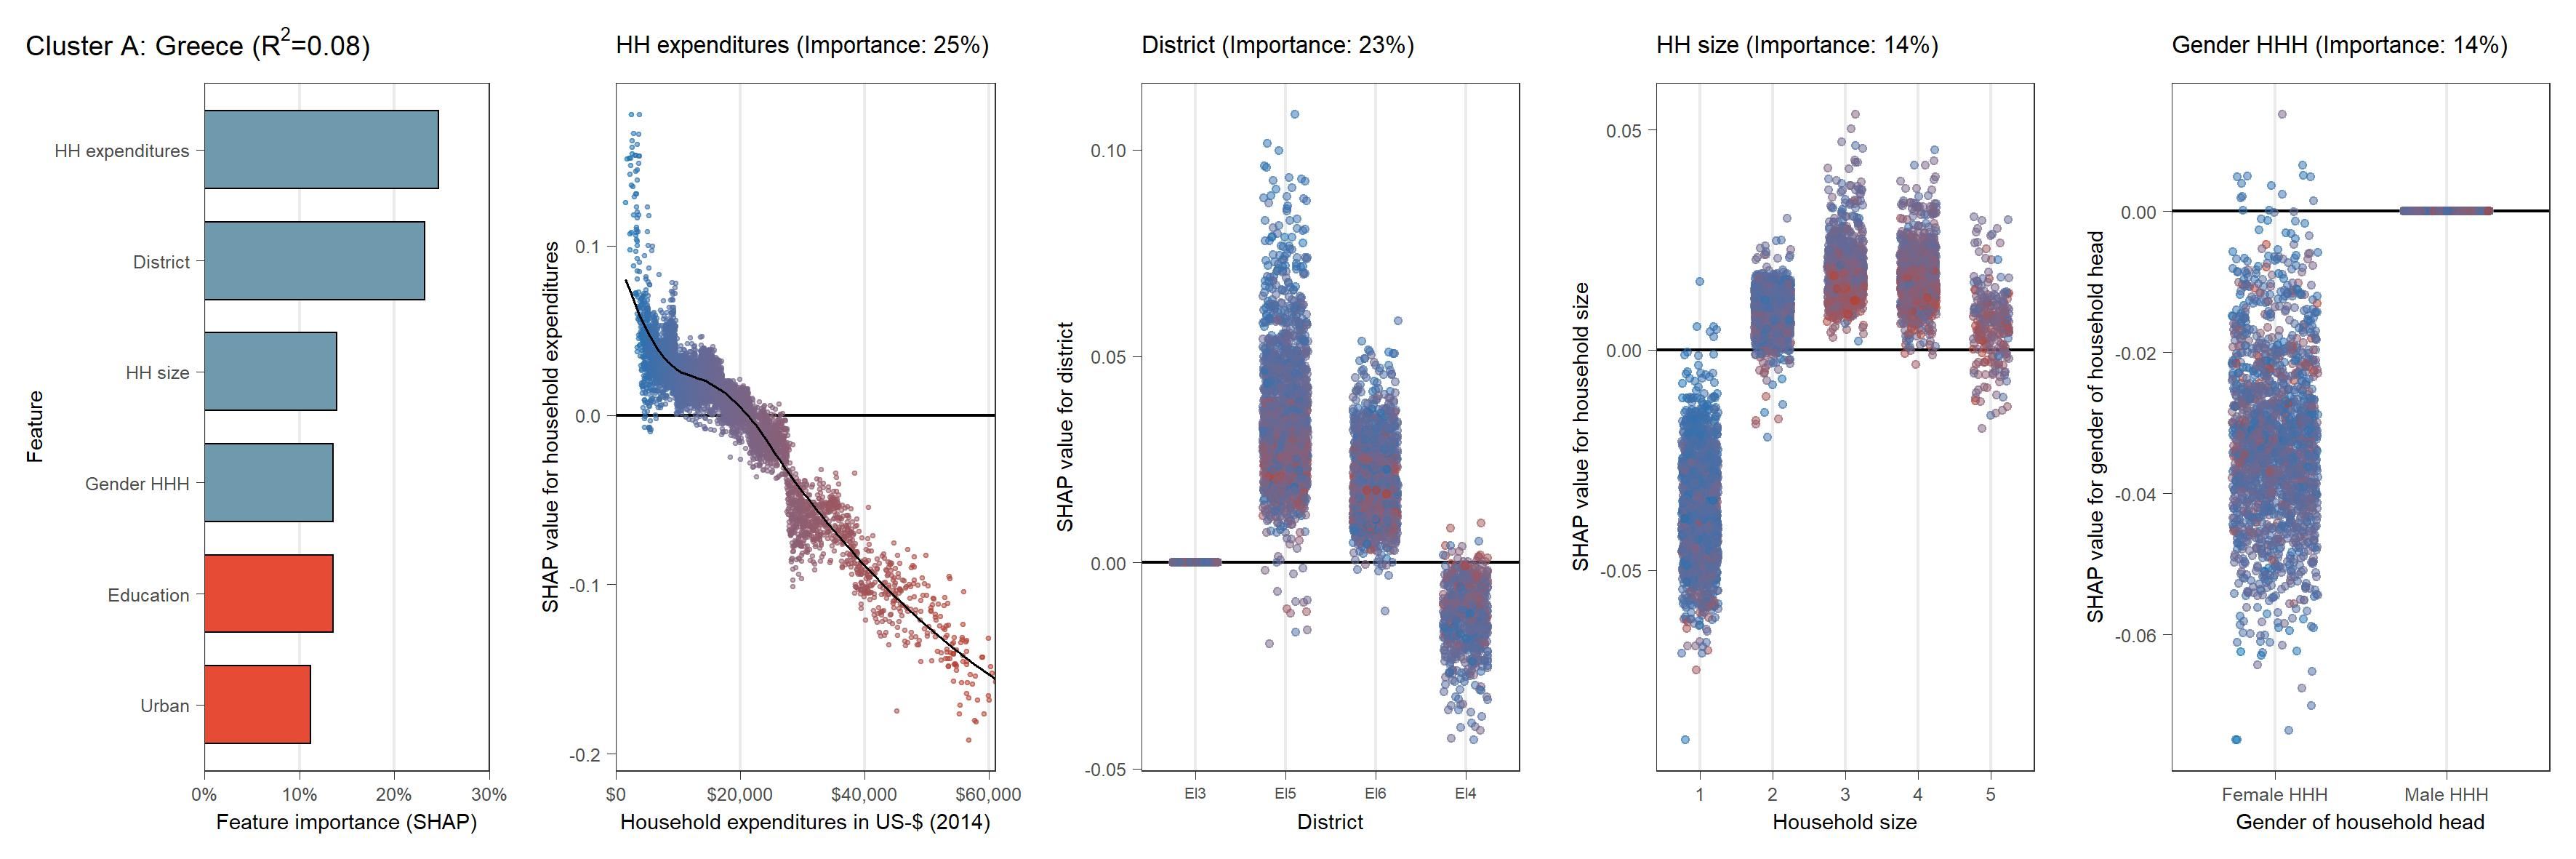
\includegraphics[width=\textwidth]{Figure 5b/Figure_5b_GRC}
         \end{subfigure}
    \\
    \vspace{0.5cm}
   \begin{subfigure}[b]{\textwidth}
   \centering
         \caption{Partial dependence plot (SHAP) for Croatia (cluster A)}
         \label{fig:5b_HRV}
         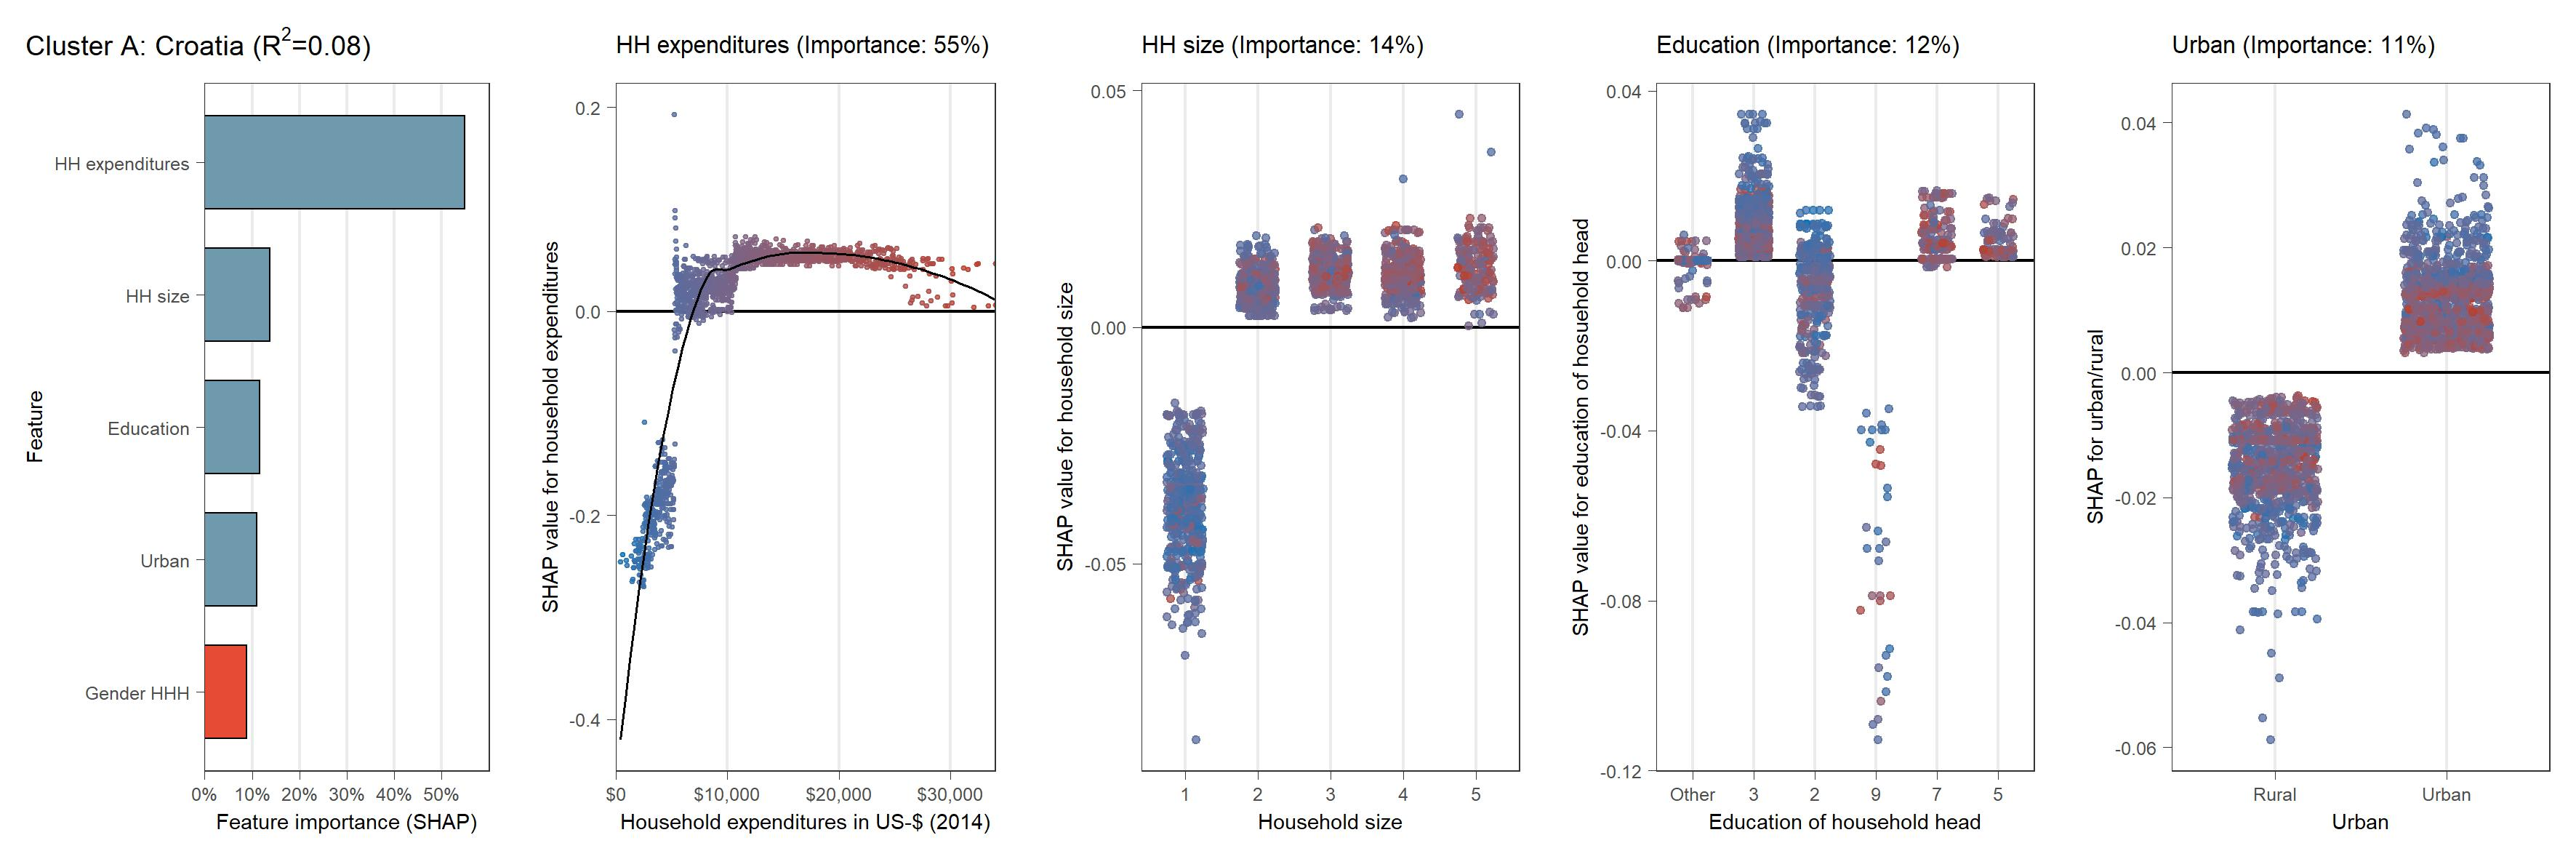
\includegraphics[width=\textwidth]{Figure 5b/Figure_5b_HRV}     
     \end{subfigure}
    \\
    \vspace{0.5cm}
   \begin{subfigure}[b]{\textwidth}
     \centering
         \caption{Partial dependence plot (SHAP) for Hungary (cluster A)}
         \label{fig:5b_HUN}
         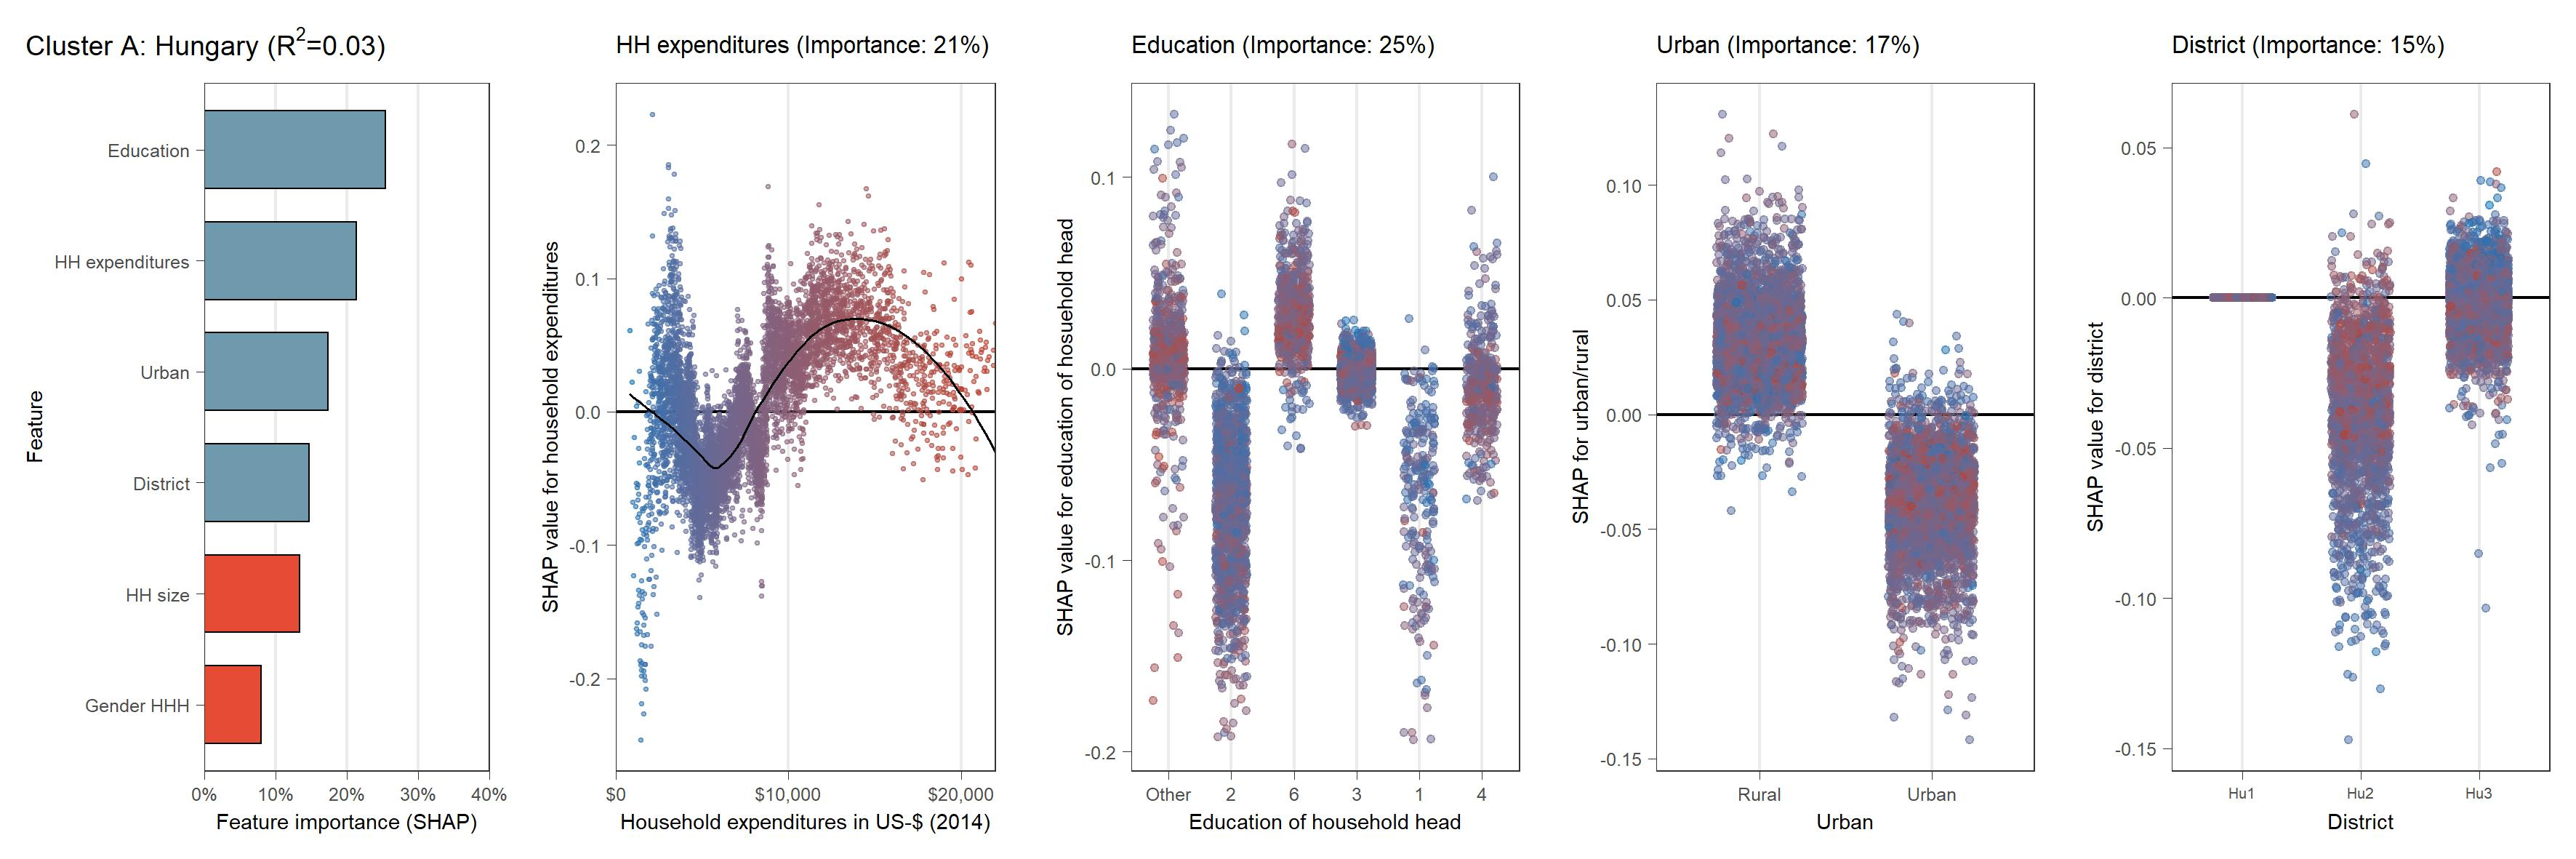
\includegraphics[width=\textwidth]{Figure 5b/Figure_5b_HUN}
    \end{subfigure}
    \\
    \vspace{0.5cm}
    \begin{subcaption2}
     This figure shows SHAP-values for predicting carbon intensity over feature values for 87 countries in order of nine country-clusters and silhouette width. The bar chart displays normalized average absolute SHAP-values for all features. Features with less than 3\% of normalized SHAP-values are subsumed as "Other features (Sum)". Charts show SHAP-values over total household expenditures for all countries and for the three most important features in each country besides total household expenditures. Colors represent household expenditures with blue (red) colors indicating lower (higher) household expenditures.
     \end{subcaption2}
\end{figure}

\begin{figure}[ht!]\ContinuedFloat
    \centering
   \begin{subfigure}[b]{\textwidth}
      \centering
         \caption{Partial dependence plot (SHAP) for Ireland (cluster A)}
         \label{fig:5b_IRL}
         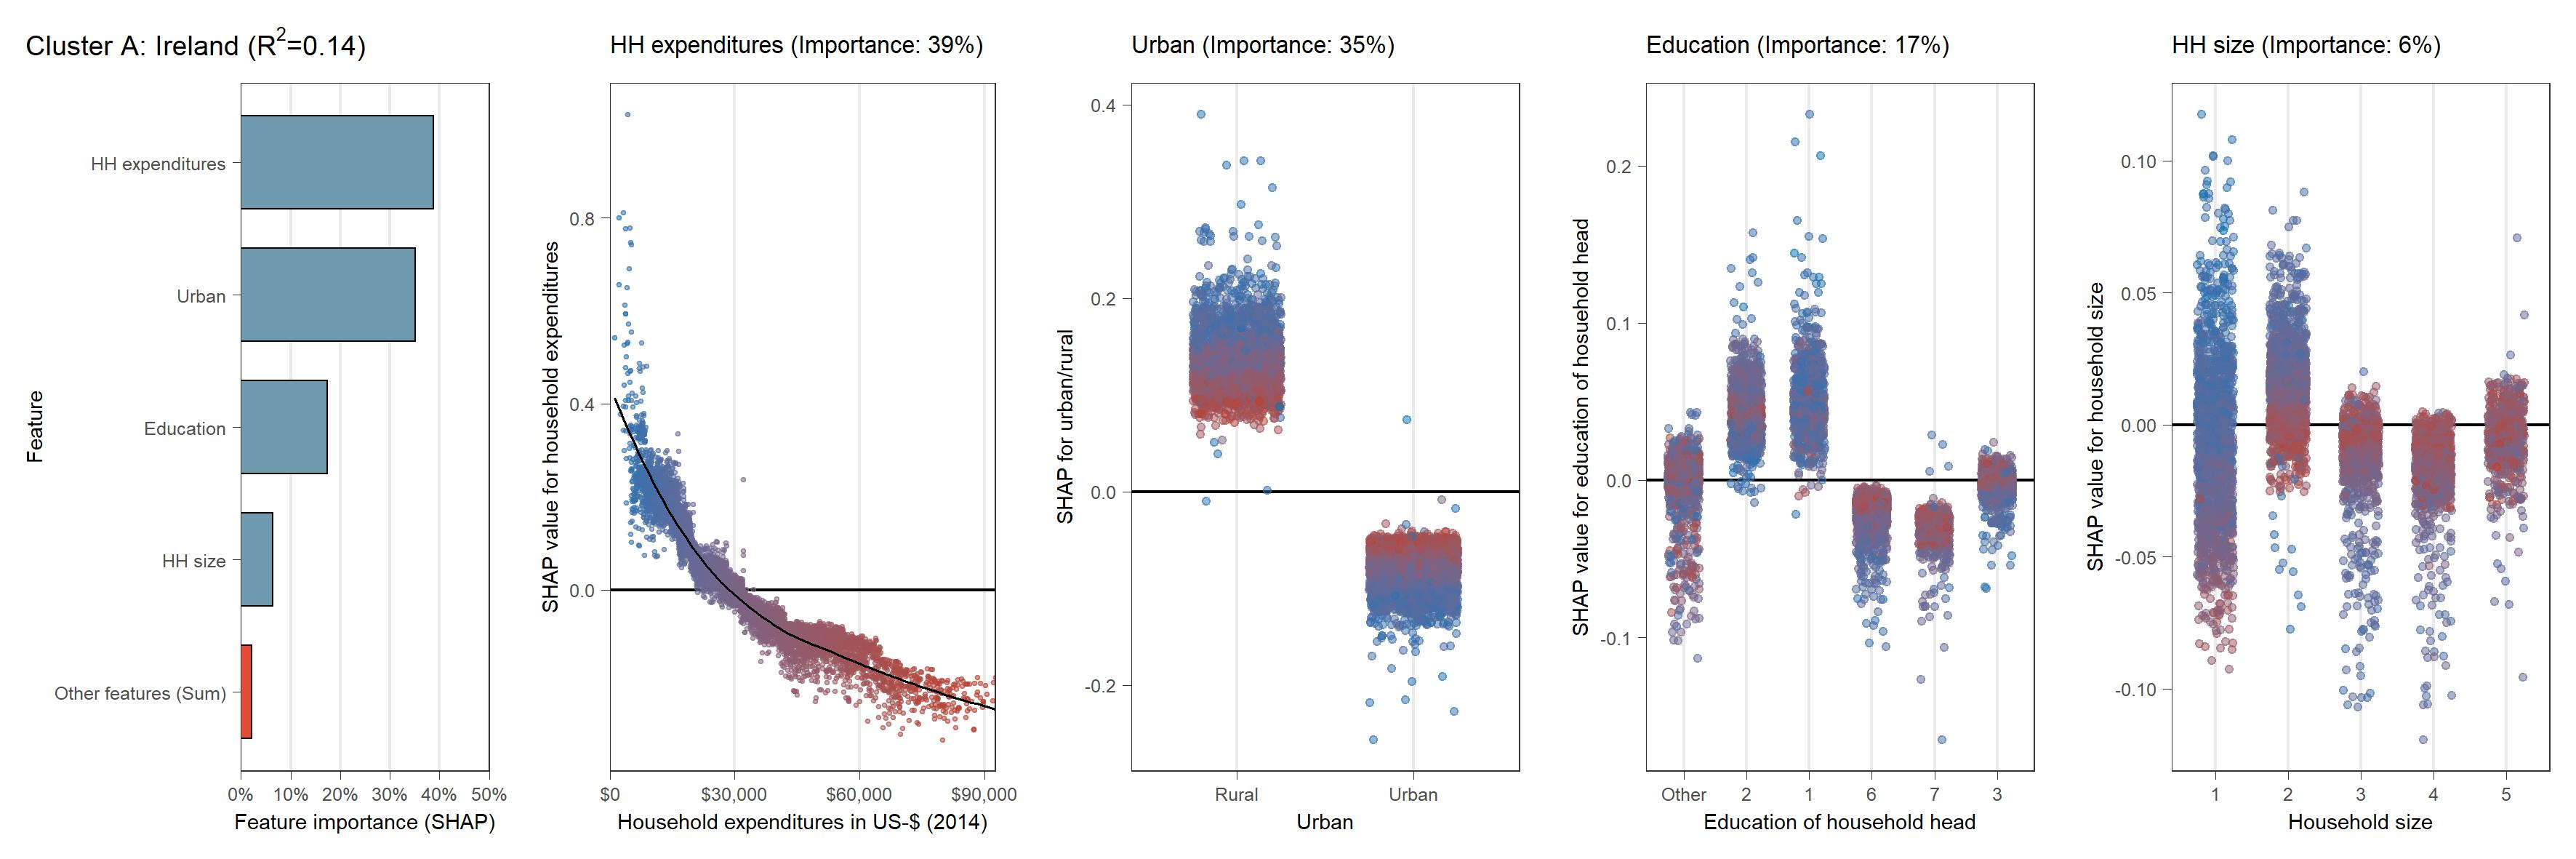
\includegraphics[width=\textwidth]{Figure 5b/Figure_5b_IRL}   
     \end{subfigure}
    \\
    \vspace{0.5cm}
   \begin{subfigure}[b]{\textwidth}
   \centering
         \caption{Partial dependence plot (SHAP) for Israel (cluster A)}
         \label{fig:5b_ISR}
         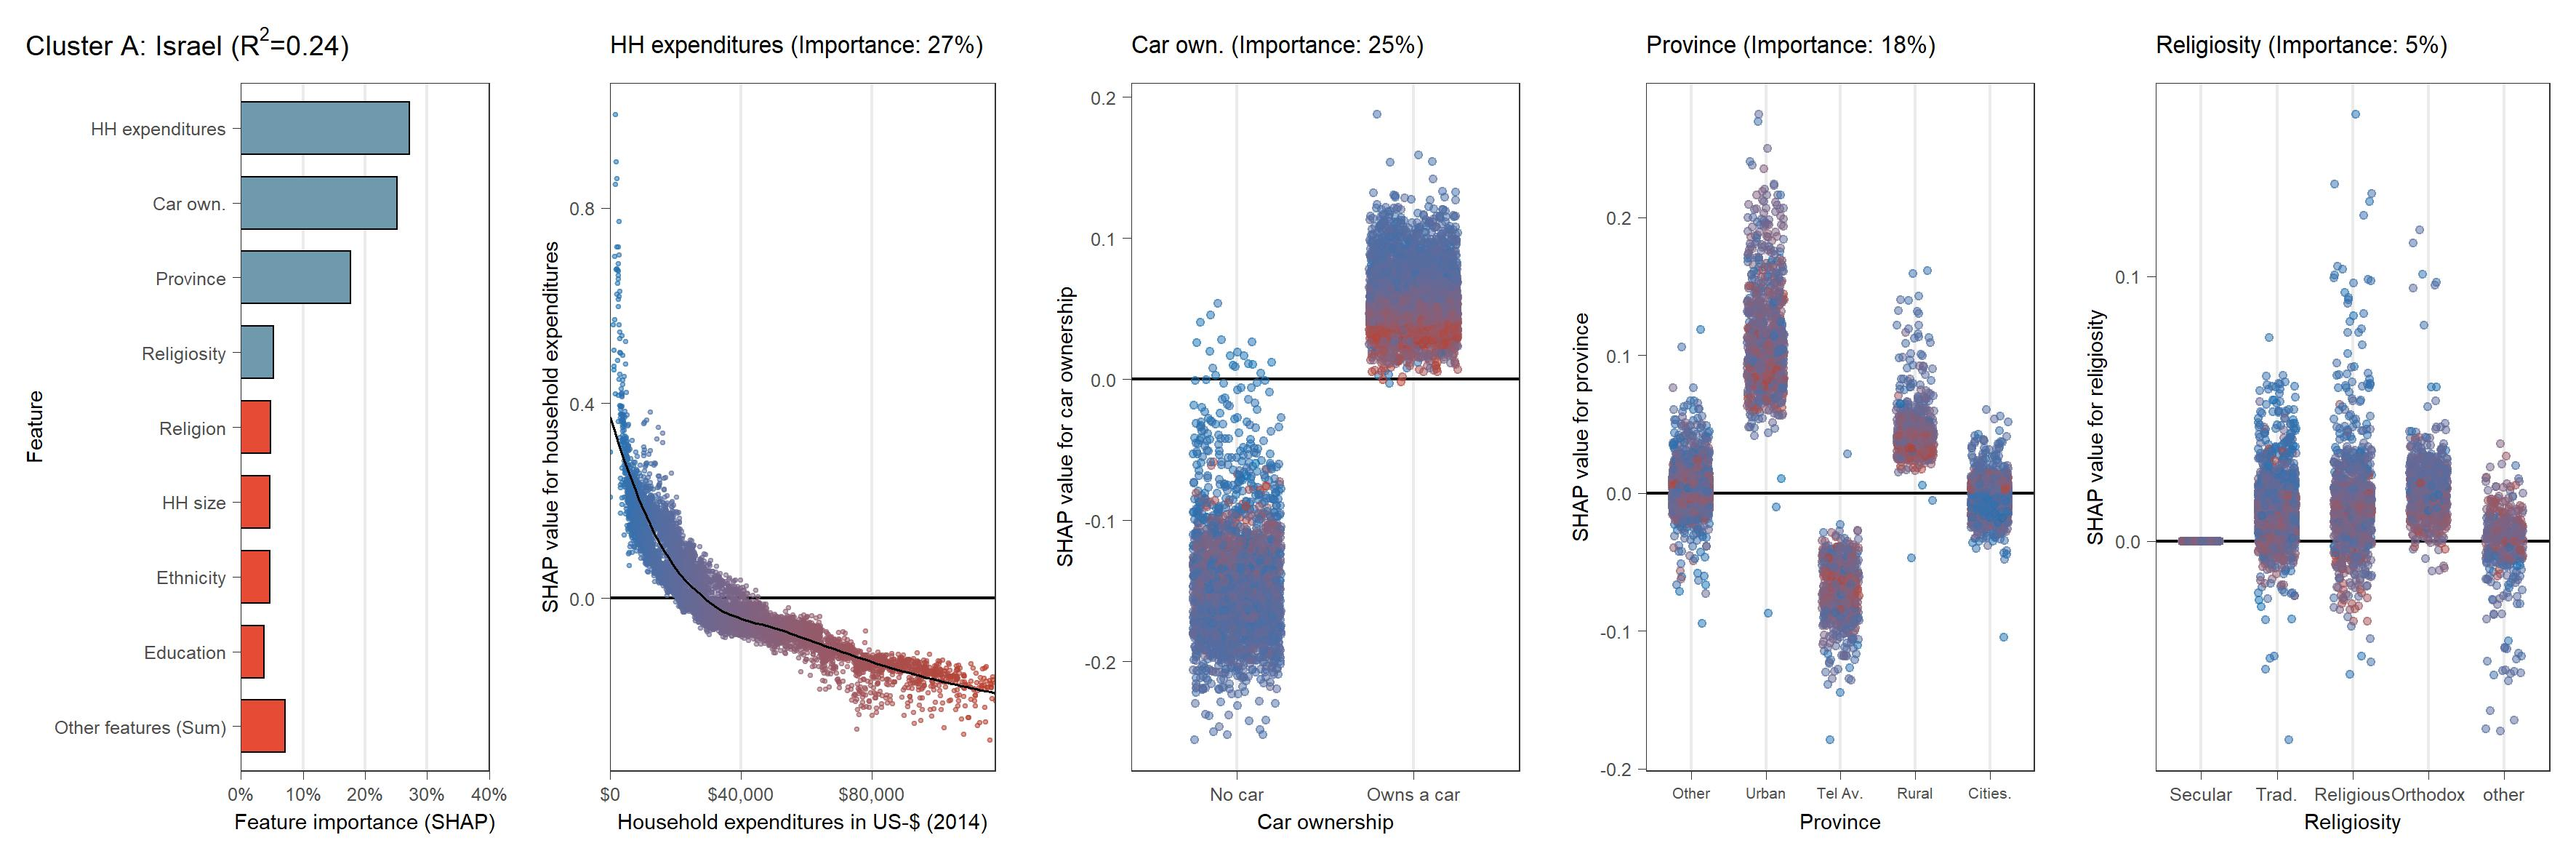
\includegraphics[width=\textwidth]{Figure 5b/Figure_5b_ISR}
         \end{subfigure}
    \\
    \vspace{0.5cm}
   \begin{subfigure}[b]{\textwidth}
         \centering
         \caption{Partial dependence plot (SHAP) for Italy (cluster A)}
         \label{fig:5b_ITA}
         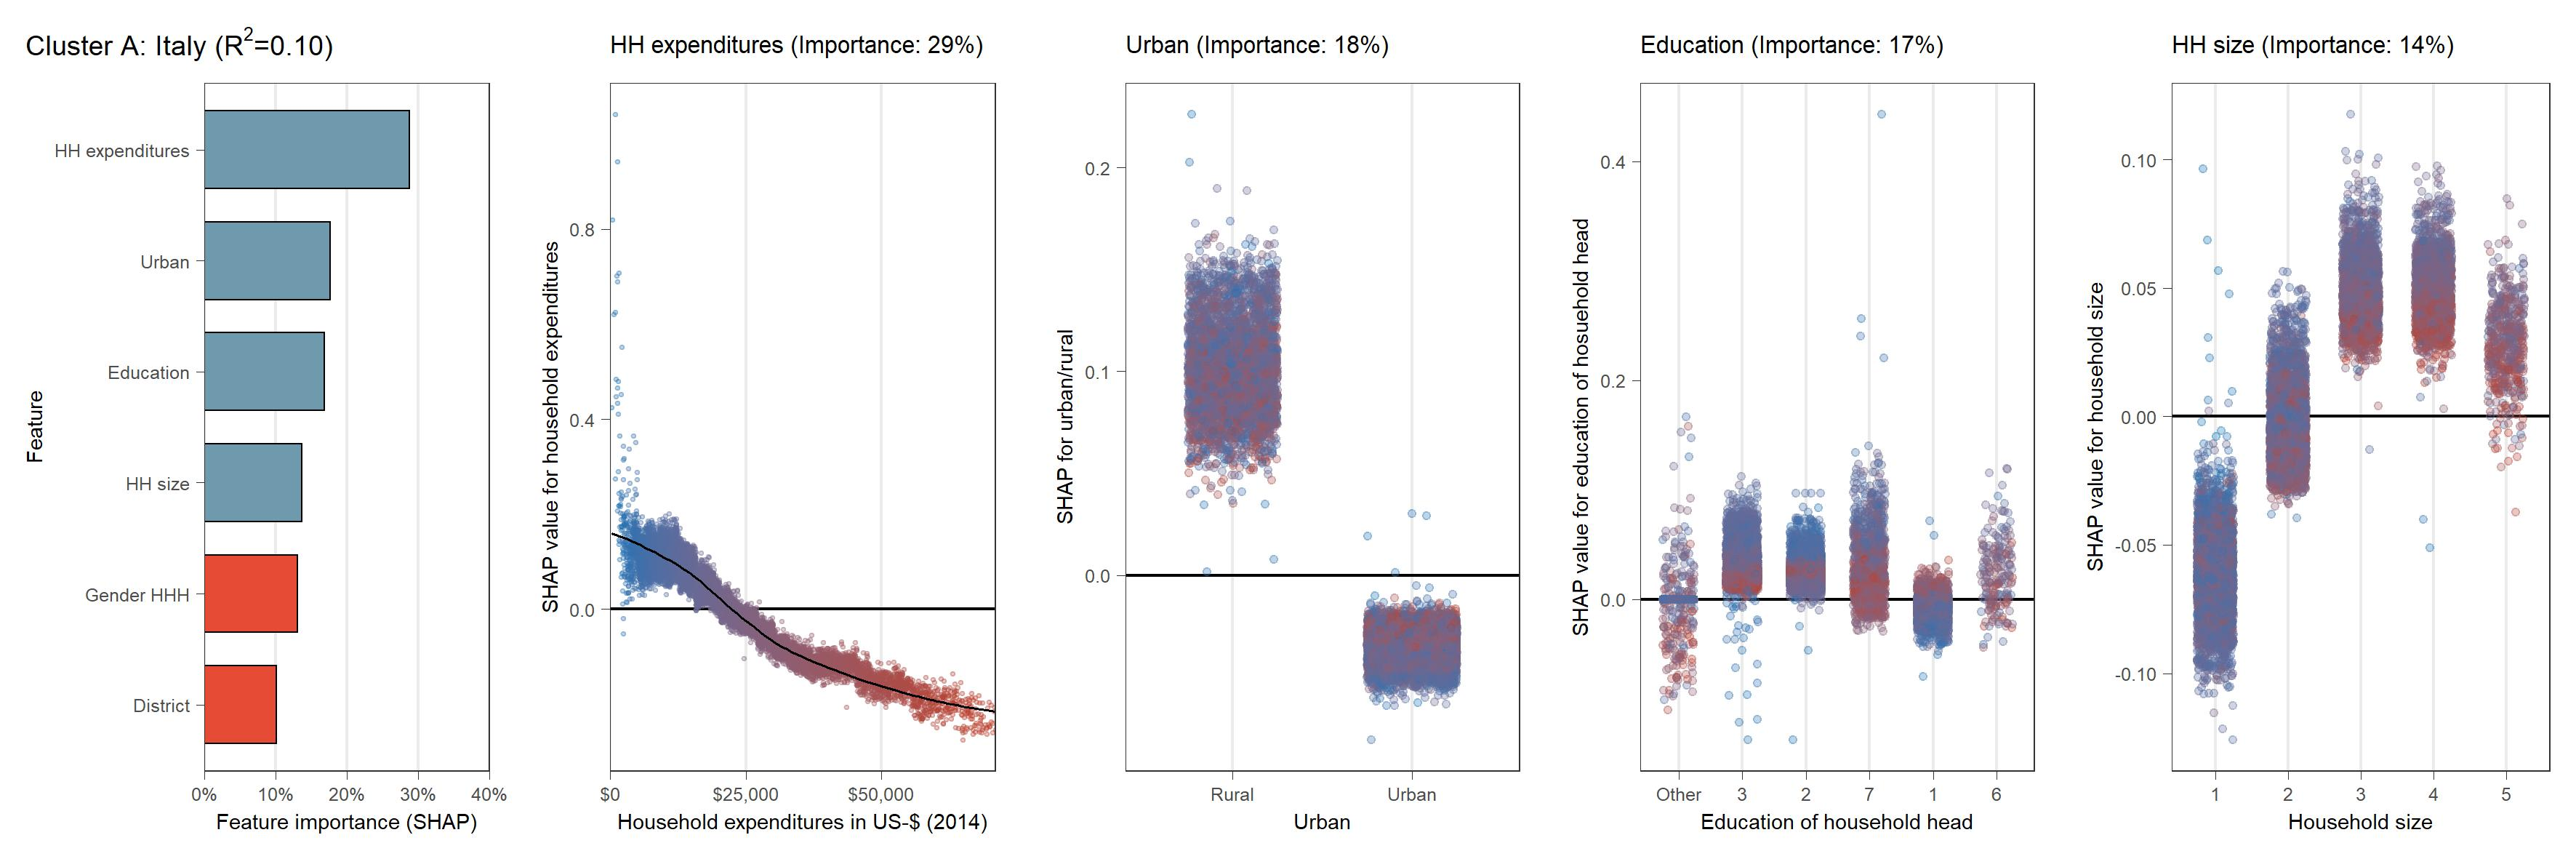
\includegraphics[width=\textwidth]{Figure 5b/Figure_5b_ITA}     
    \end{subfigure}
    \\
    \vspace{0.5cm}
    \begin{subcaption2}
     This figure shows SHAP-values for predicting carbon intensity over feature values for 87 countries in order of nine country-clusters and silhouette width. The bar chart displays normalized average absolute SHAP-values for all features. Features with less than 3\% of normalized SHAP-values are subsumed as "Other features (Sum)". Charts show SHAP-values over total household expenditures for all countries and for the three most important features in each country besides total household expenditures. Colors represent household expenditures with blue (red) colors indicating lower (higher) household expenditures.
     \end{subcaption2}
\end{figure}

\begin{figure}[ht!]\ContinuedFloat
    \centering
   \begin{subfigure}[b]{\textwidth}
         \centering
         \caption{Partial dependence plot (SHAP) for Kenya (cluster A)}
         \label{fig:5b_KEN}
         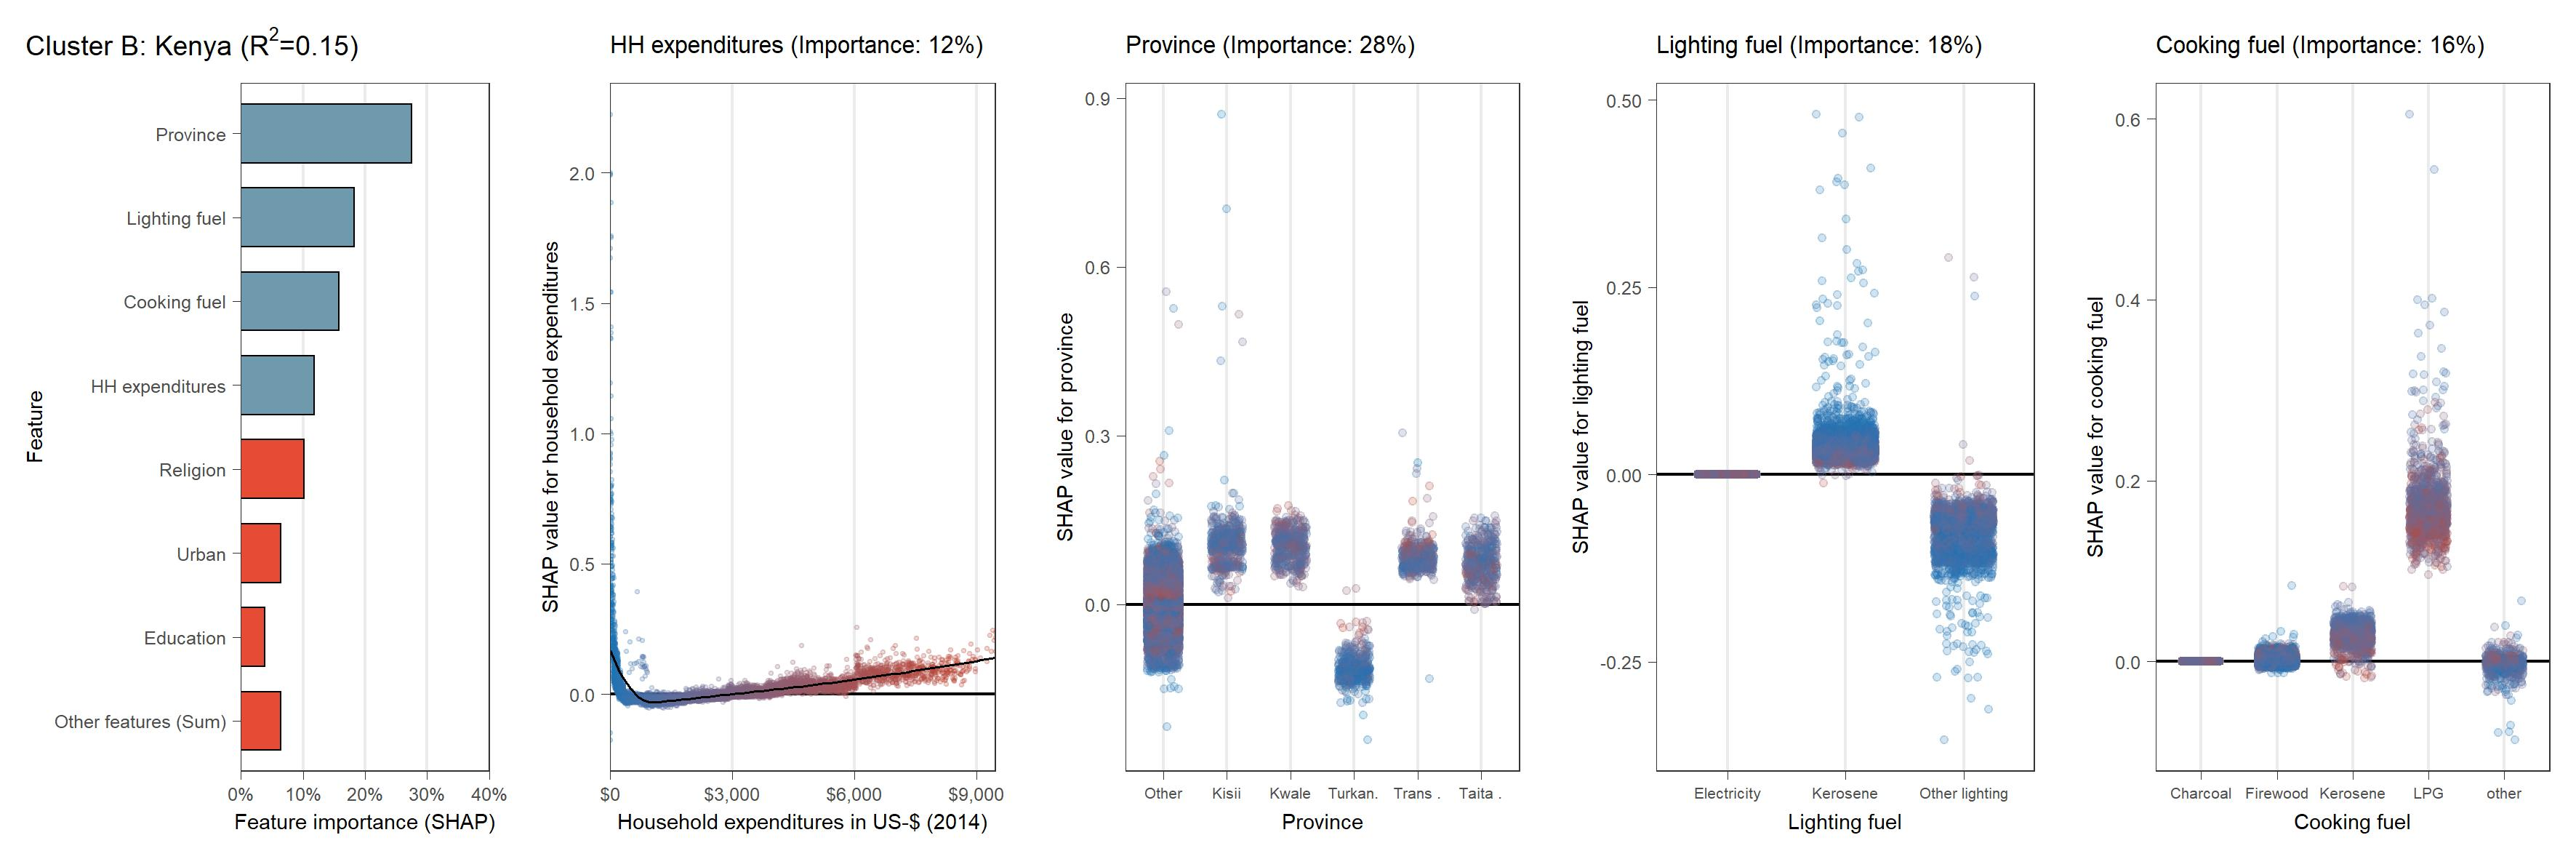
\includegraphics[width=\textwidth]{Figure 5b/Figure_5b_KEN}     
         \end{subfigure}
    \\
    \vspace{0.5cm}
   \begin{subfigure}[b]{\textwidth}        
         \centering
         \caption{Partial dependence plot (SHAP) for Cambodia (cluster A)}
         \label{fig:5b_KHM}
         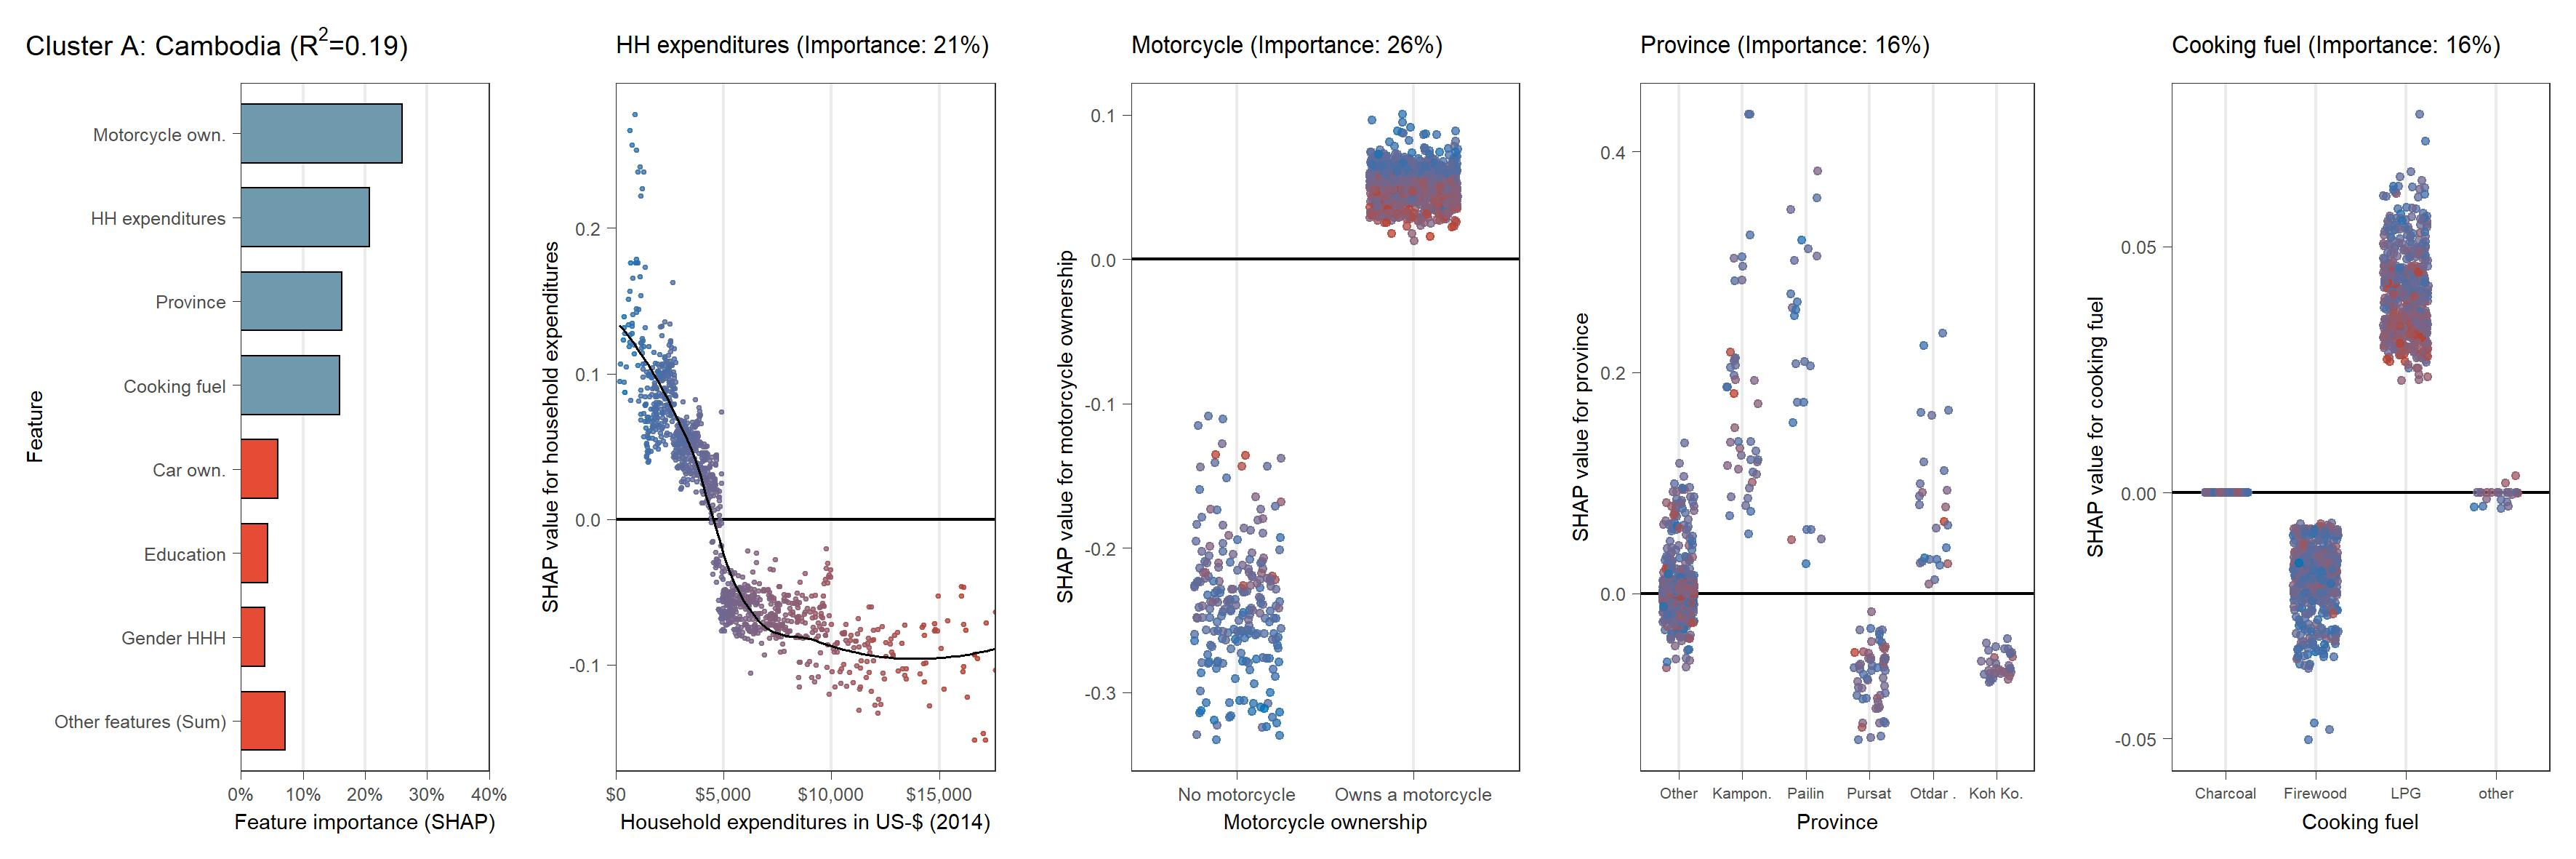
\includegraphics[width=\textwidth]{Figure 5b/Figure_5b_KHM}
         \end{subfigure}
    \\
    \vspace{0.5cm}
   \begin{subfigure}[b]{\textwidth}      
         \centering
         \caption{Partial dependence plot (SHAP) for Lithuania (cluster A)}
         \label{fig:5b_LTU}
         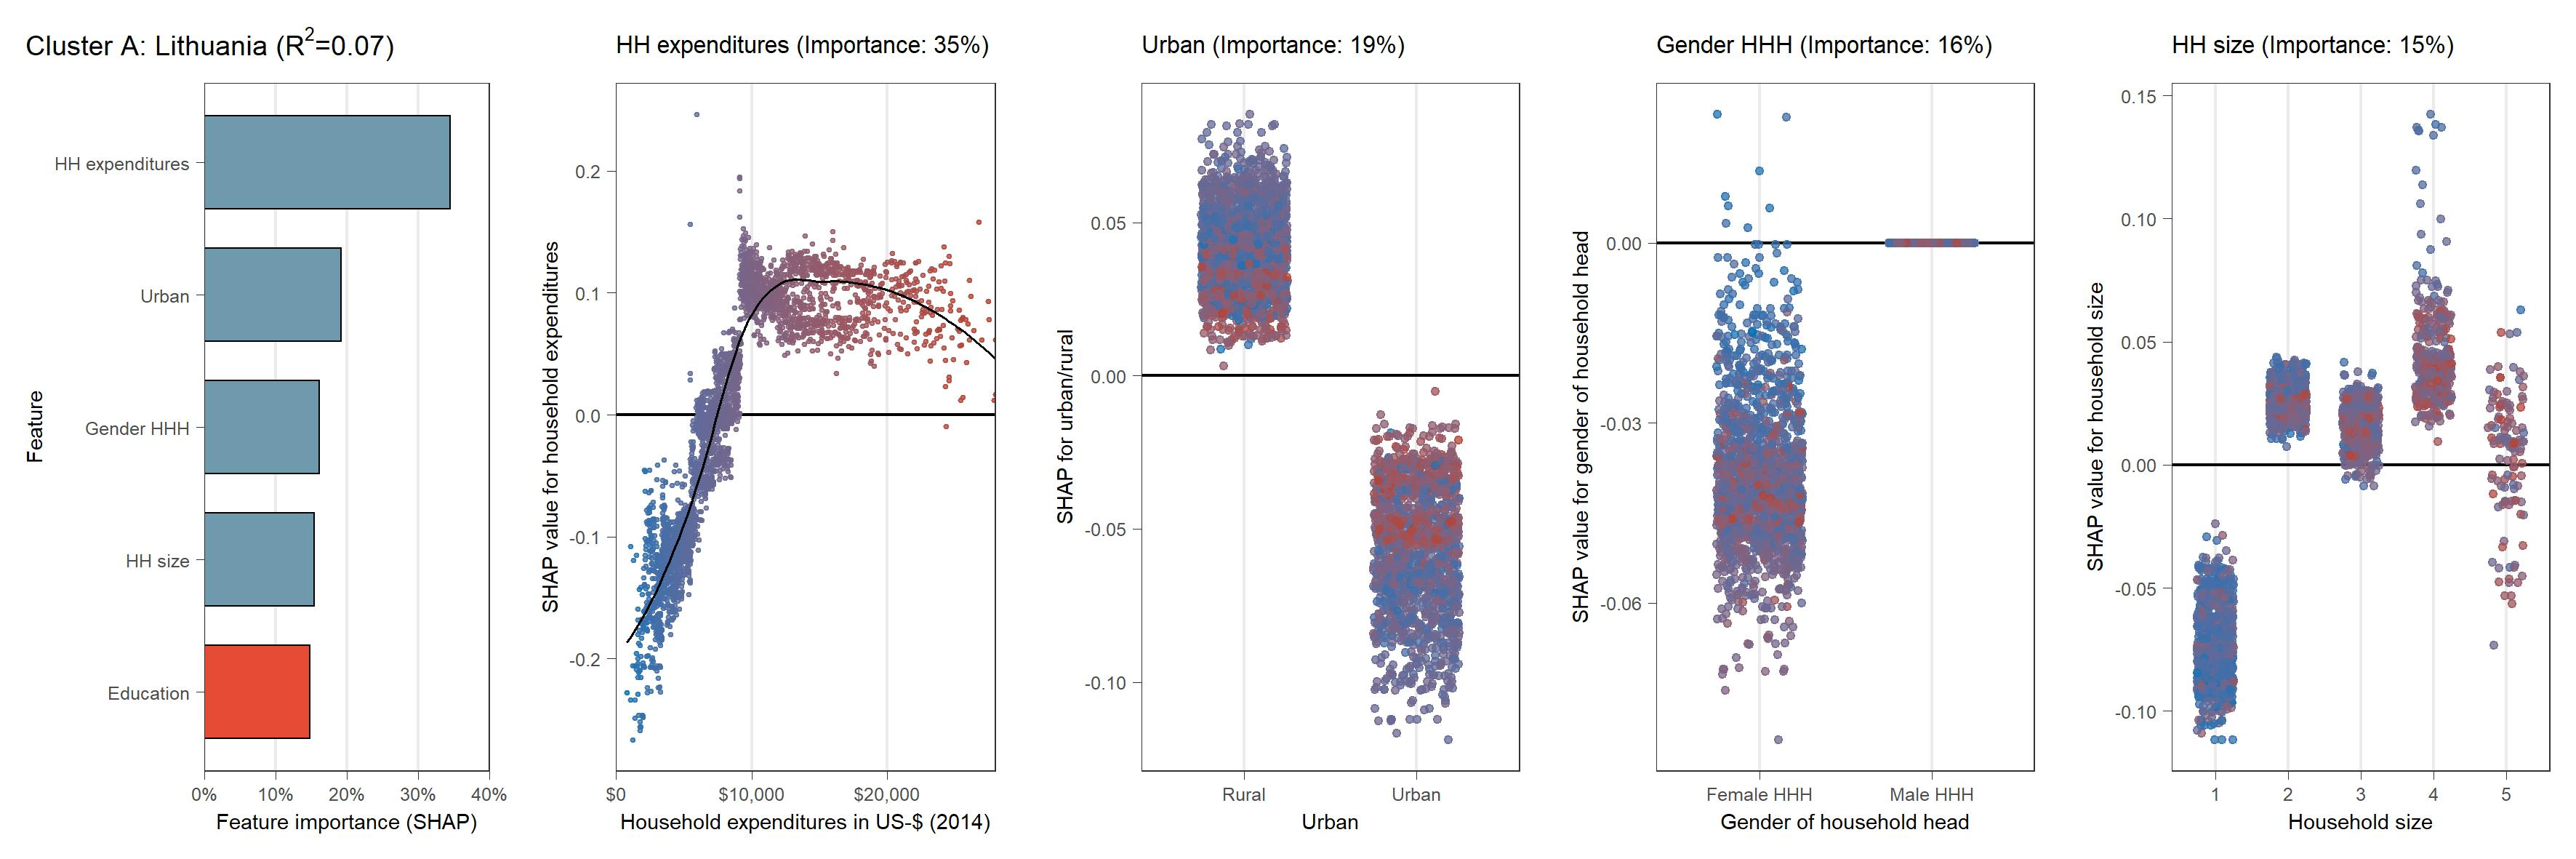
\includegraphics[width=\textwidth]{Figure 5b/Figure_5b_LTU} 
         \end{subfigure}
    \\
    \vspace{0.5cm}
    \begin{subcaption2}
     This figure shows SHAP-values for predicting carbon intensity over feature values for 87 countries in order of nine country-clusters and silhouette width. The bar chart displays normalized average absolute SHAP-values for all features. Features with less than 3\% of normalized SHAP-values are subsumed as "Other features (Sum)". Charts show SHAP-values over total household expenditures for all countries and for the three most important features in each country besides total household expenditures. Colors represent household expenditures with blue (red) colors indicating lower (higher) household expenditures.
     \end{subcaption2}
\end{figure}

\begin{figure}[ht!]\ContinuedFloat
    \centering
   \begin{subfigure}[b]{\textwidth}
         \centering
         \caption{Partial dependence plot (SHAP) for Luxembourg (cluster A)}
         \label{fig:5b_LUX}
         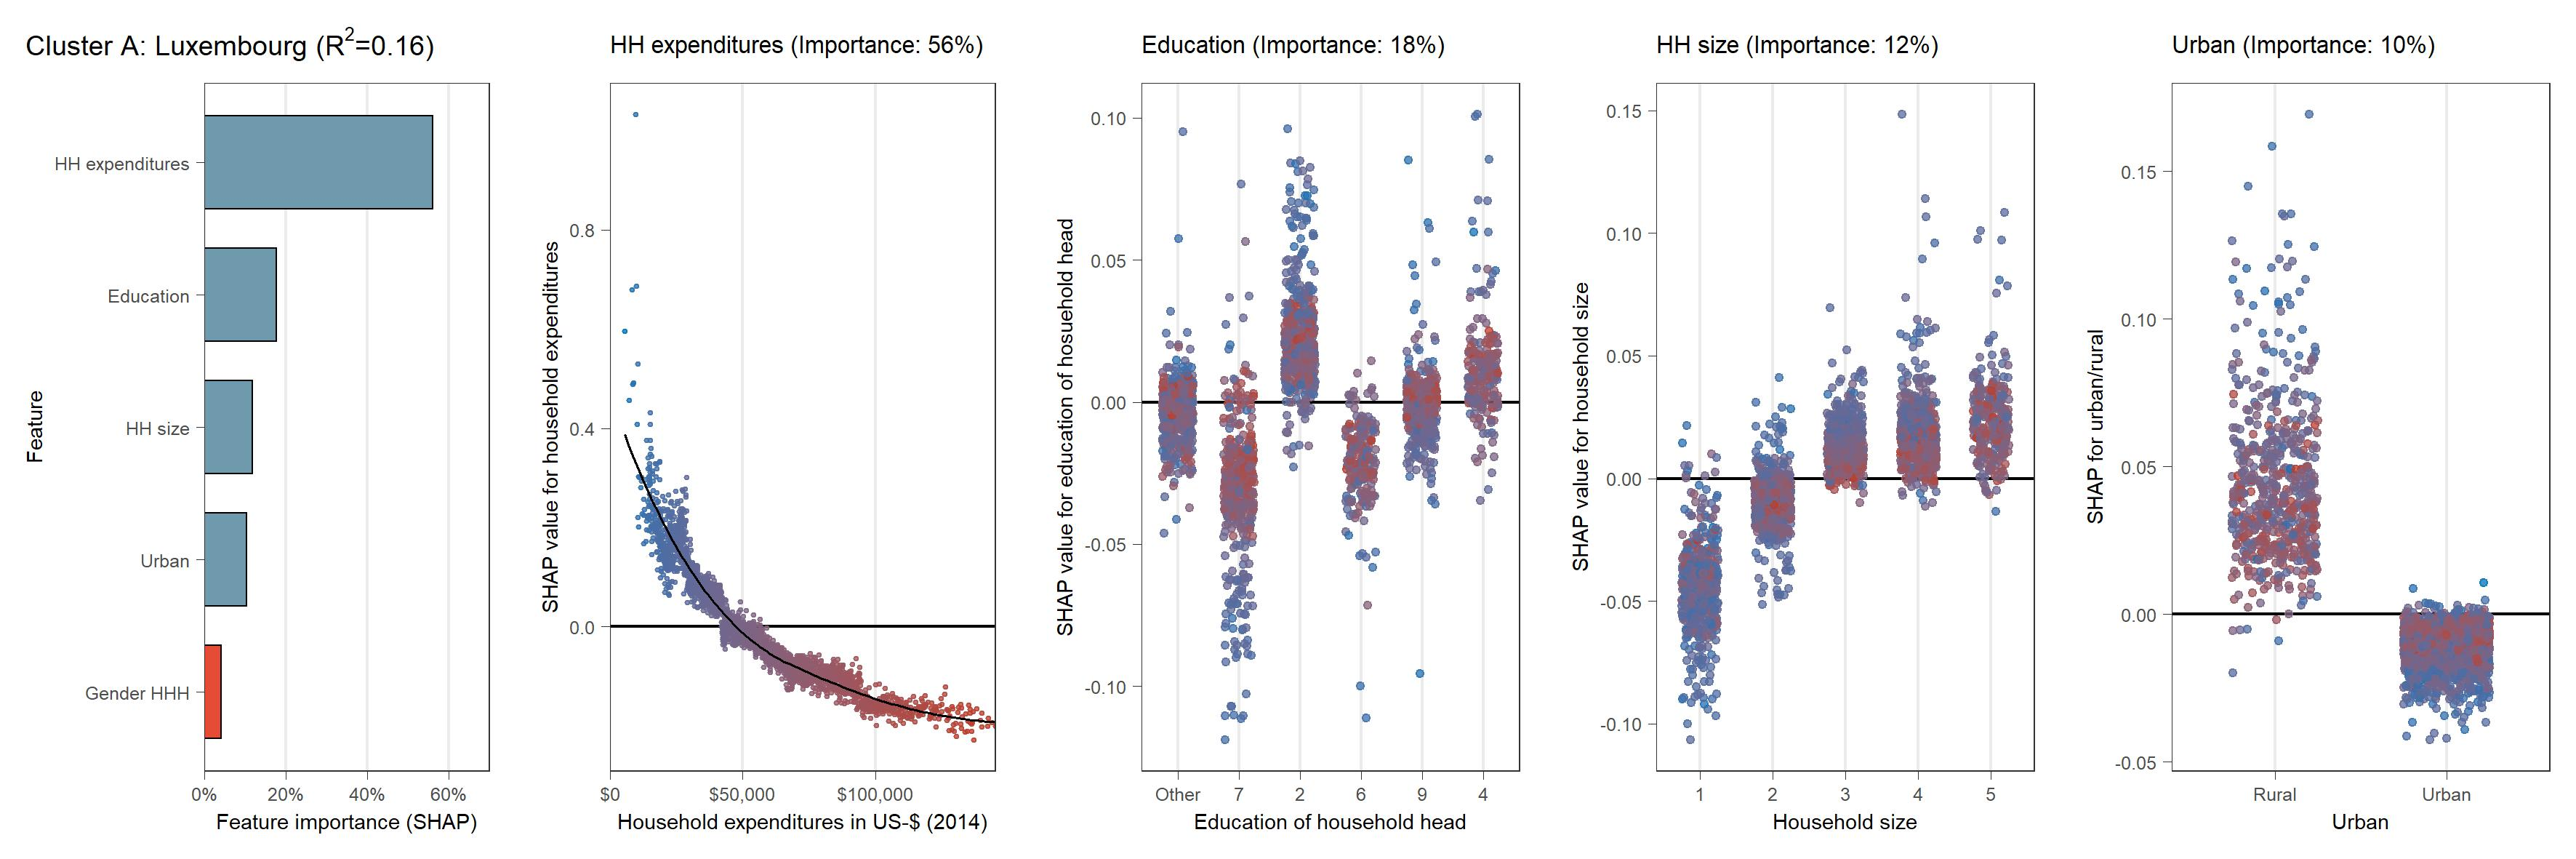
\includegraphics[width=\textwidth]{Figure 5b/Figure_5b_LUX}
         \end{subfigure}
    \\
    \vspace{0.5cm}
   \begin{subfigure}[b]{\textwidth}
   \centering
         \caption{Partial dependence plot (SHAP) for Latvia (cluster A)}
         \label{fig:5b_LVA}
         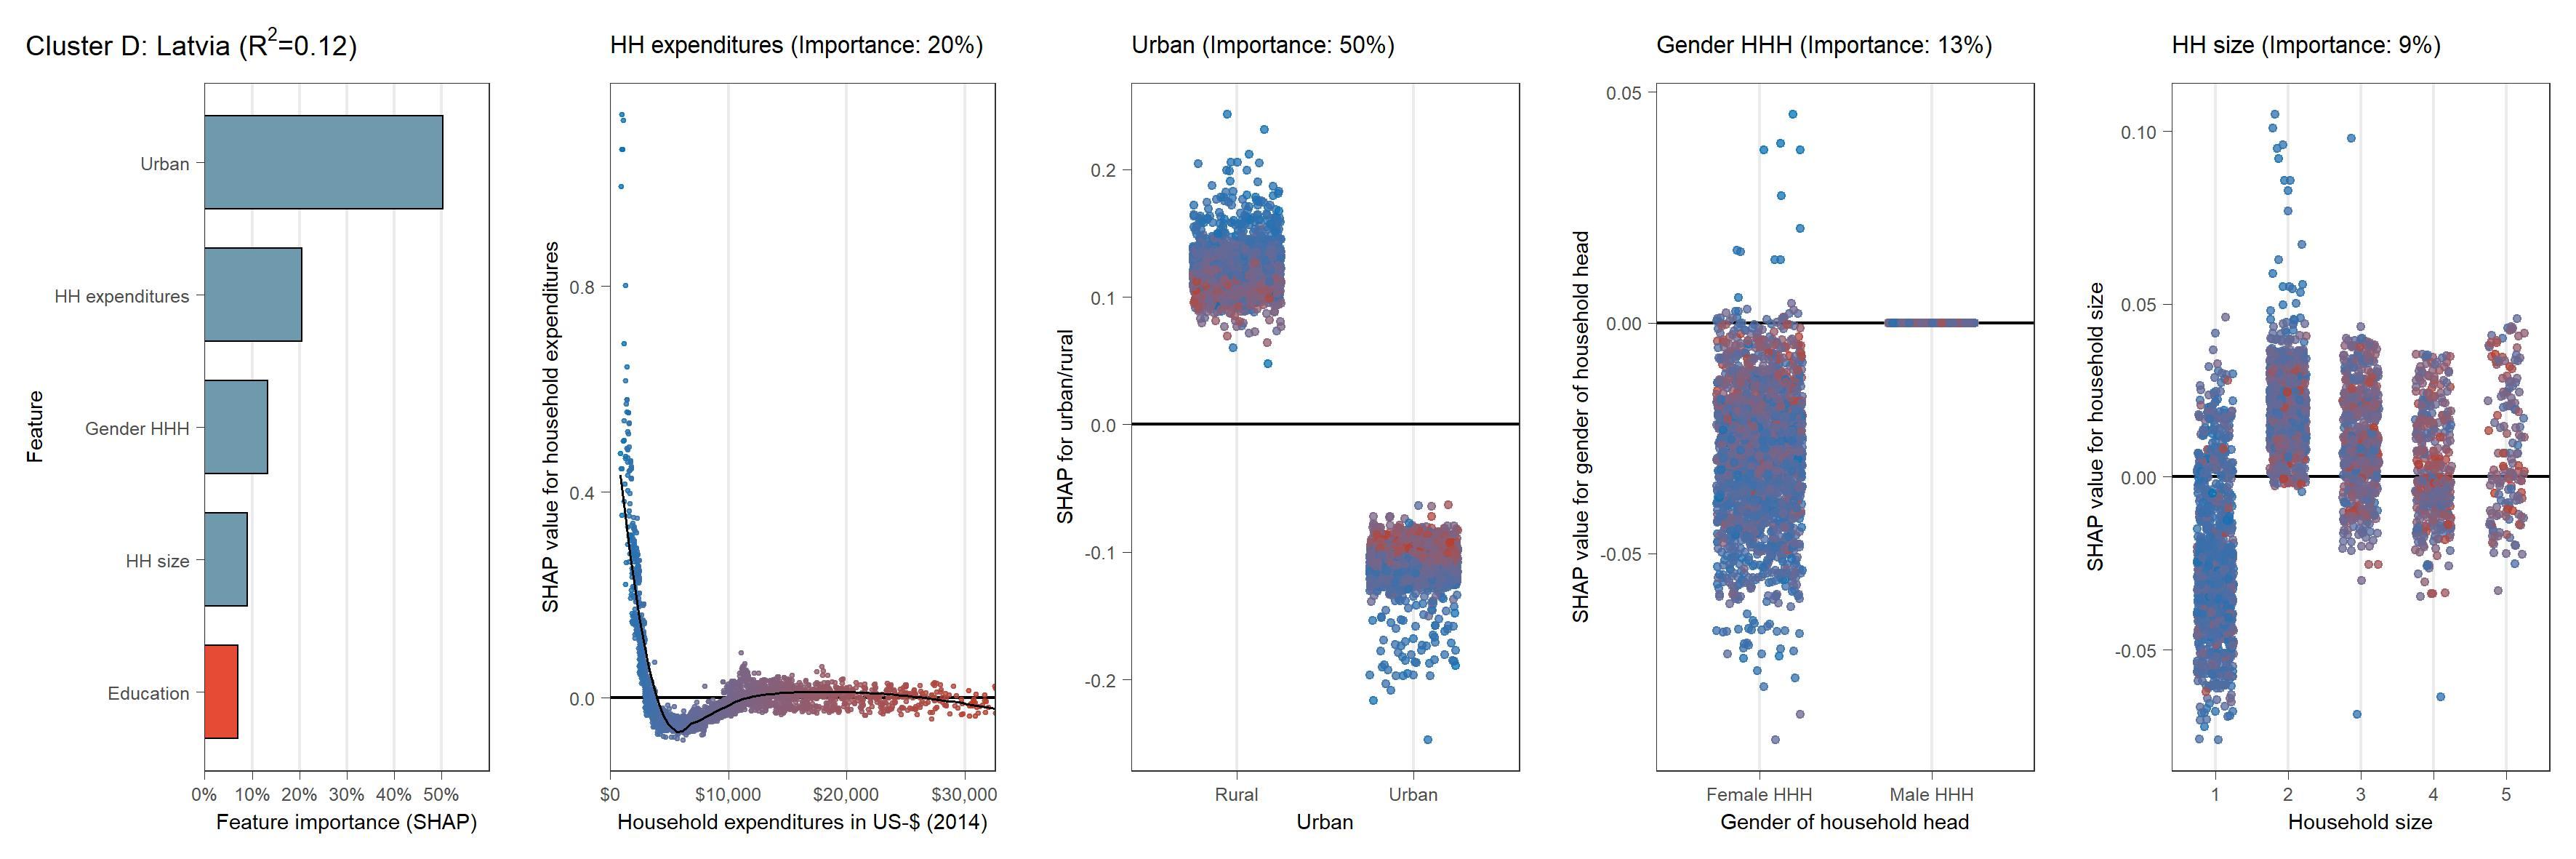
\includegraphics[width=\textwidth]{Figure 5b/Figure_5b_LVA}
         \end{subfigure}
    \\
    \vspace{0.5cm}
   \begin{subfigure}[b]{\textwidth}
    \centering
         \caption{Partial dependence plot (SHAP) for Morocco (cluster A)}
         \label{fig:5b_MAR}
         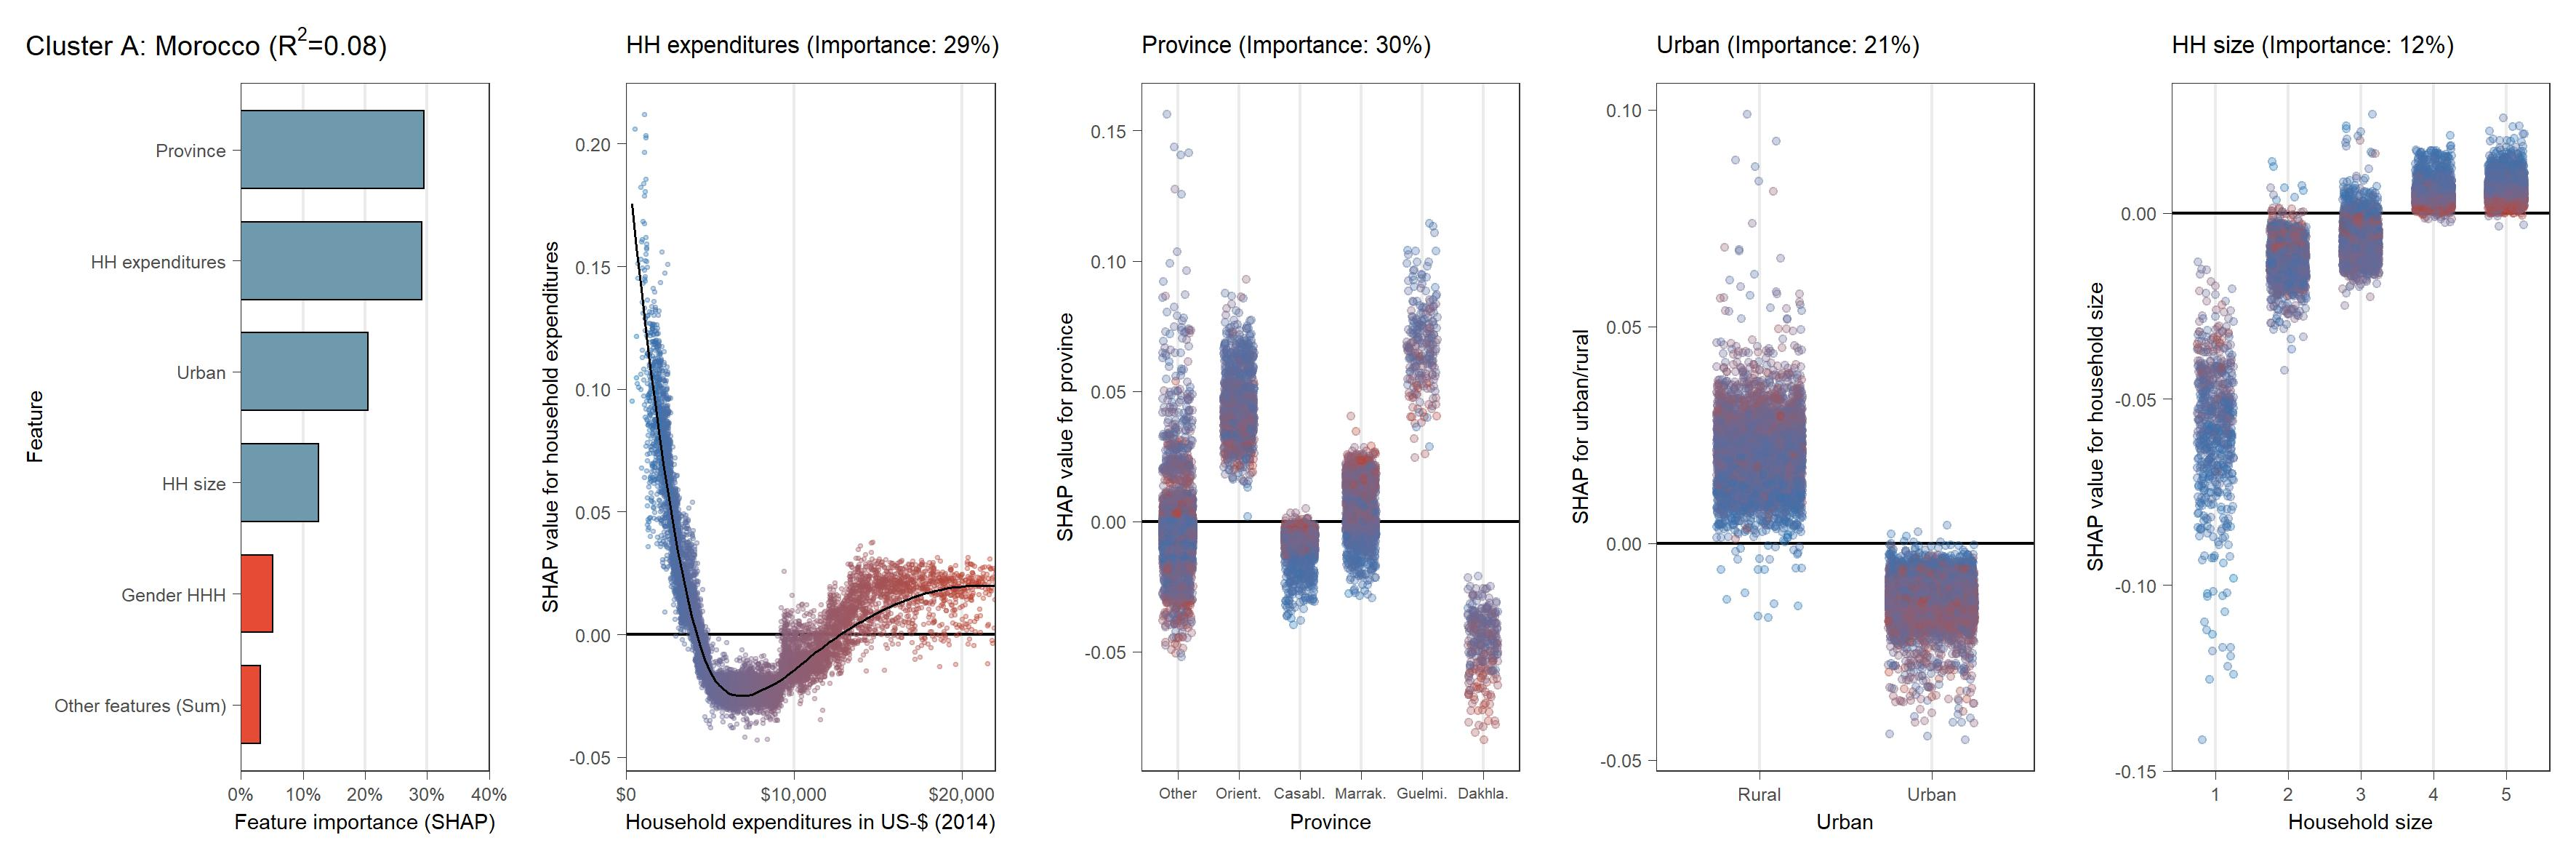
\includegraphics[width=\textwidth]{Figure 5b/Figure_5b_MAR}     
         \end{subfigure}
    \\
    \vspace{0.5cm}
    \begin{subcaption2}
     This figure shows SHAP-values for predicting carbon intensity over feature values for 87 countries in order of nine country-clusters and silhouette width. The bar chart displays normalized average absolute SHAP-values for all features. Features with less than 3\% of normalized SHAP-values are subsumed as "Other features (Sum)". Charts show SHAP-values over total household expenditures for all countries and for the three most important features in each country besides total household expenditures. Colors represent household expenditures with blue (red) colors indicating lower (higher) household expenditures.
     \end{subcaption2}
\end{figure}

\begin{figure}[ht!]\ContinuedFloat
    \centering
   \begin{subfigure}[b]{\textwidth}
    \centering
         \caption{Partial dependence plot (SHAP) for Maldives (cluster A)}
         \label{fig:5b_MDV}
         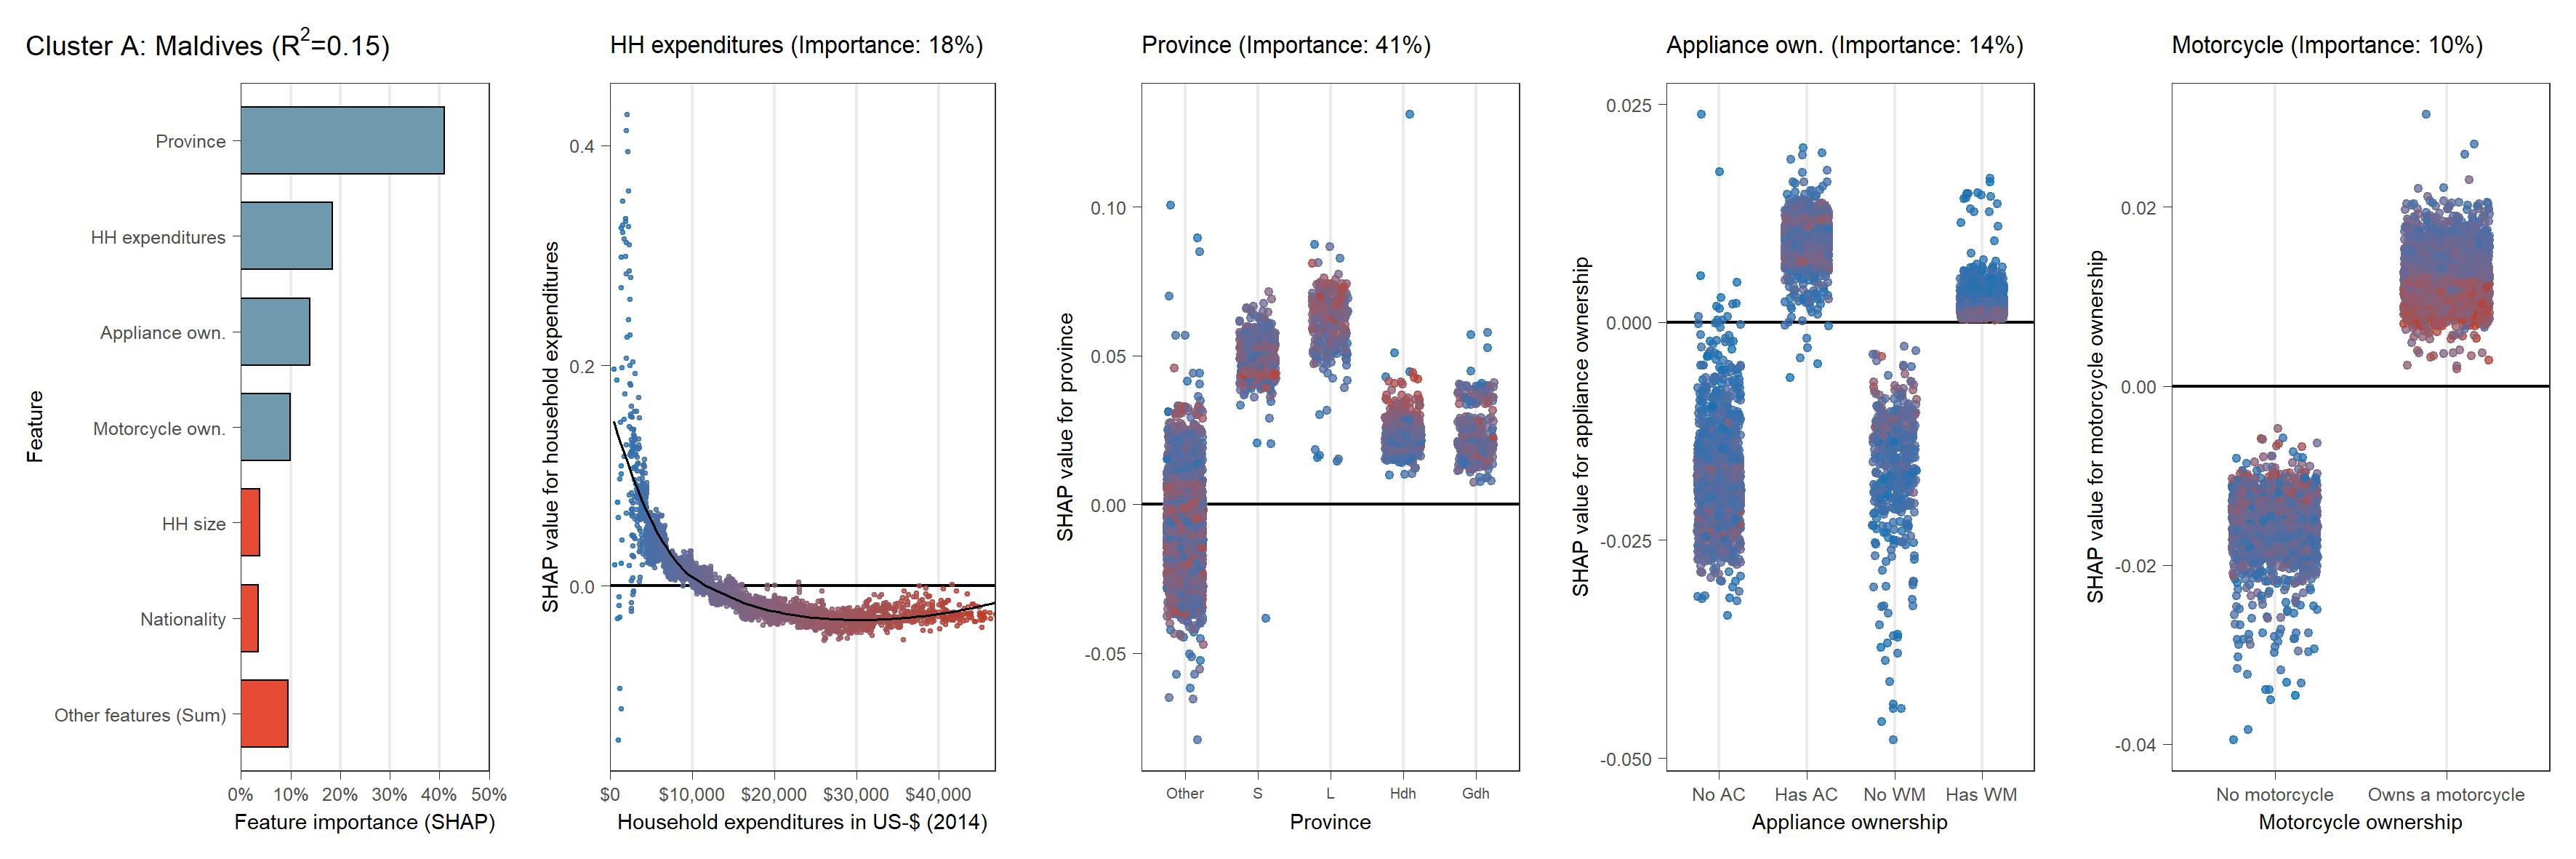
\includegraphics[width=\textwidth]{Figure 5b/Figure_5b_MDV}     
     \end{subfigure}
    \\
    \vspace{0.5cm}
   \begin{subfigure}[b]{\textwidth}
    \centering
         \caption{Partial dependence plot (SHAP) for Mongolia (cluster A)}
         \label{fig:5b_MNG}
         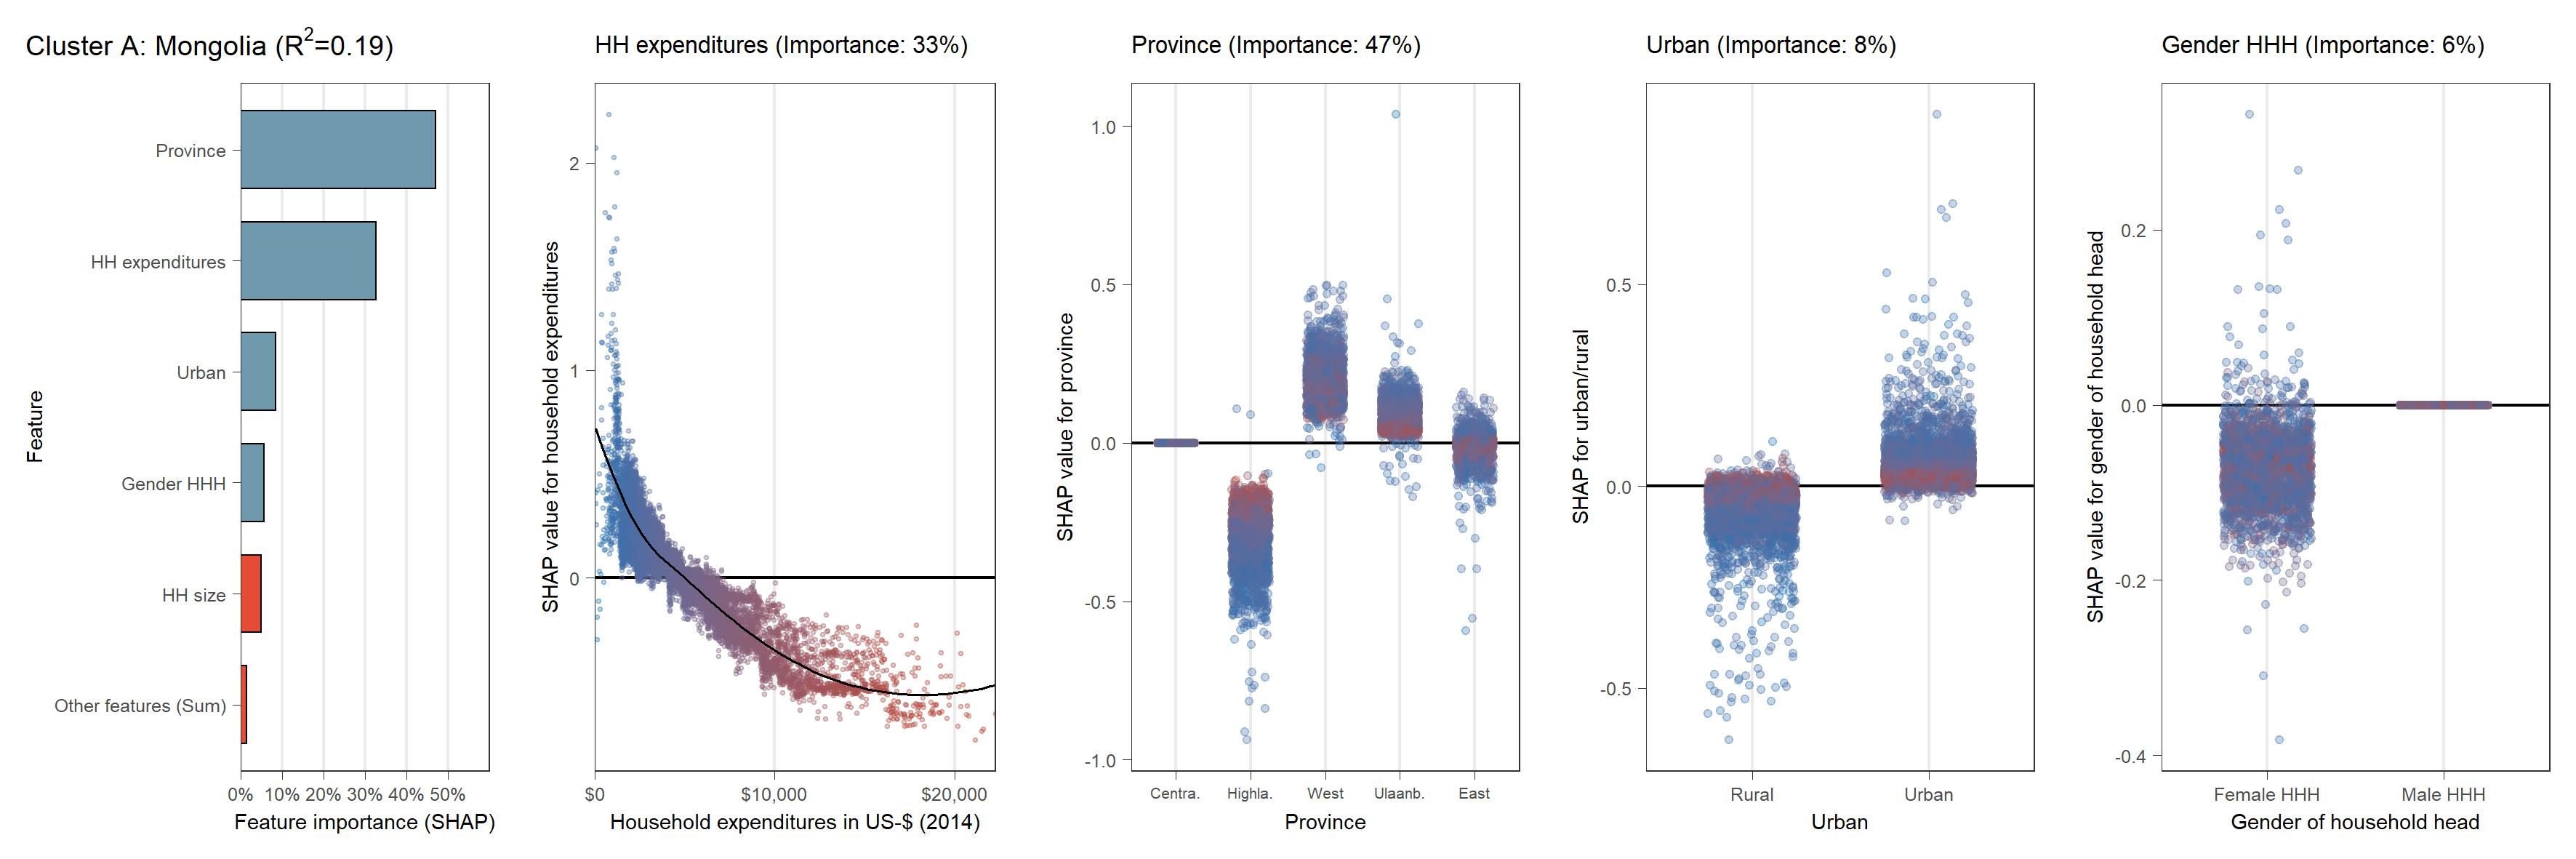
\includegraphics[width=\textwidth]{Figure 5b/Figure_5b_MNG}     
         \end{subfigure}
    \\
    \vspace{0.5cm}
   \begin{subfigure}[b]{\textwidth}
   \centering
         \caption{Partial dependence plot (SHAP) for the Netherlands (cluster A)}
         \label{fig:5b_NLD}
         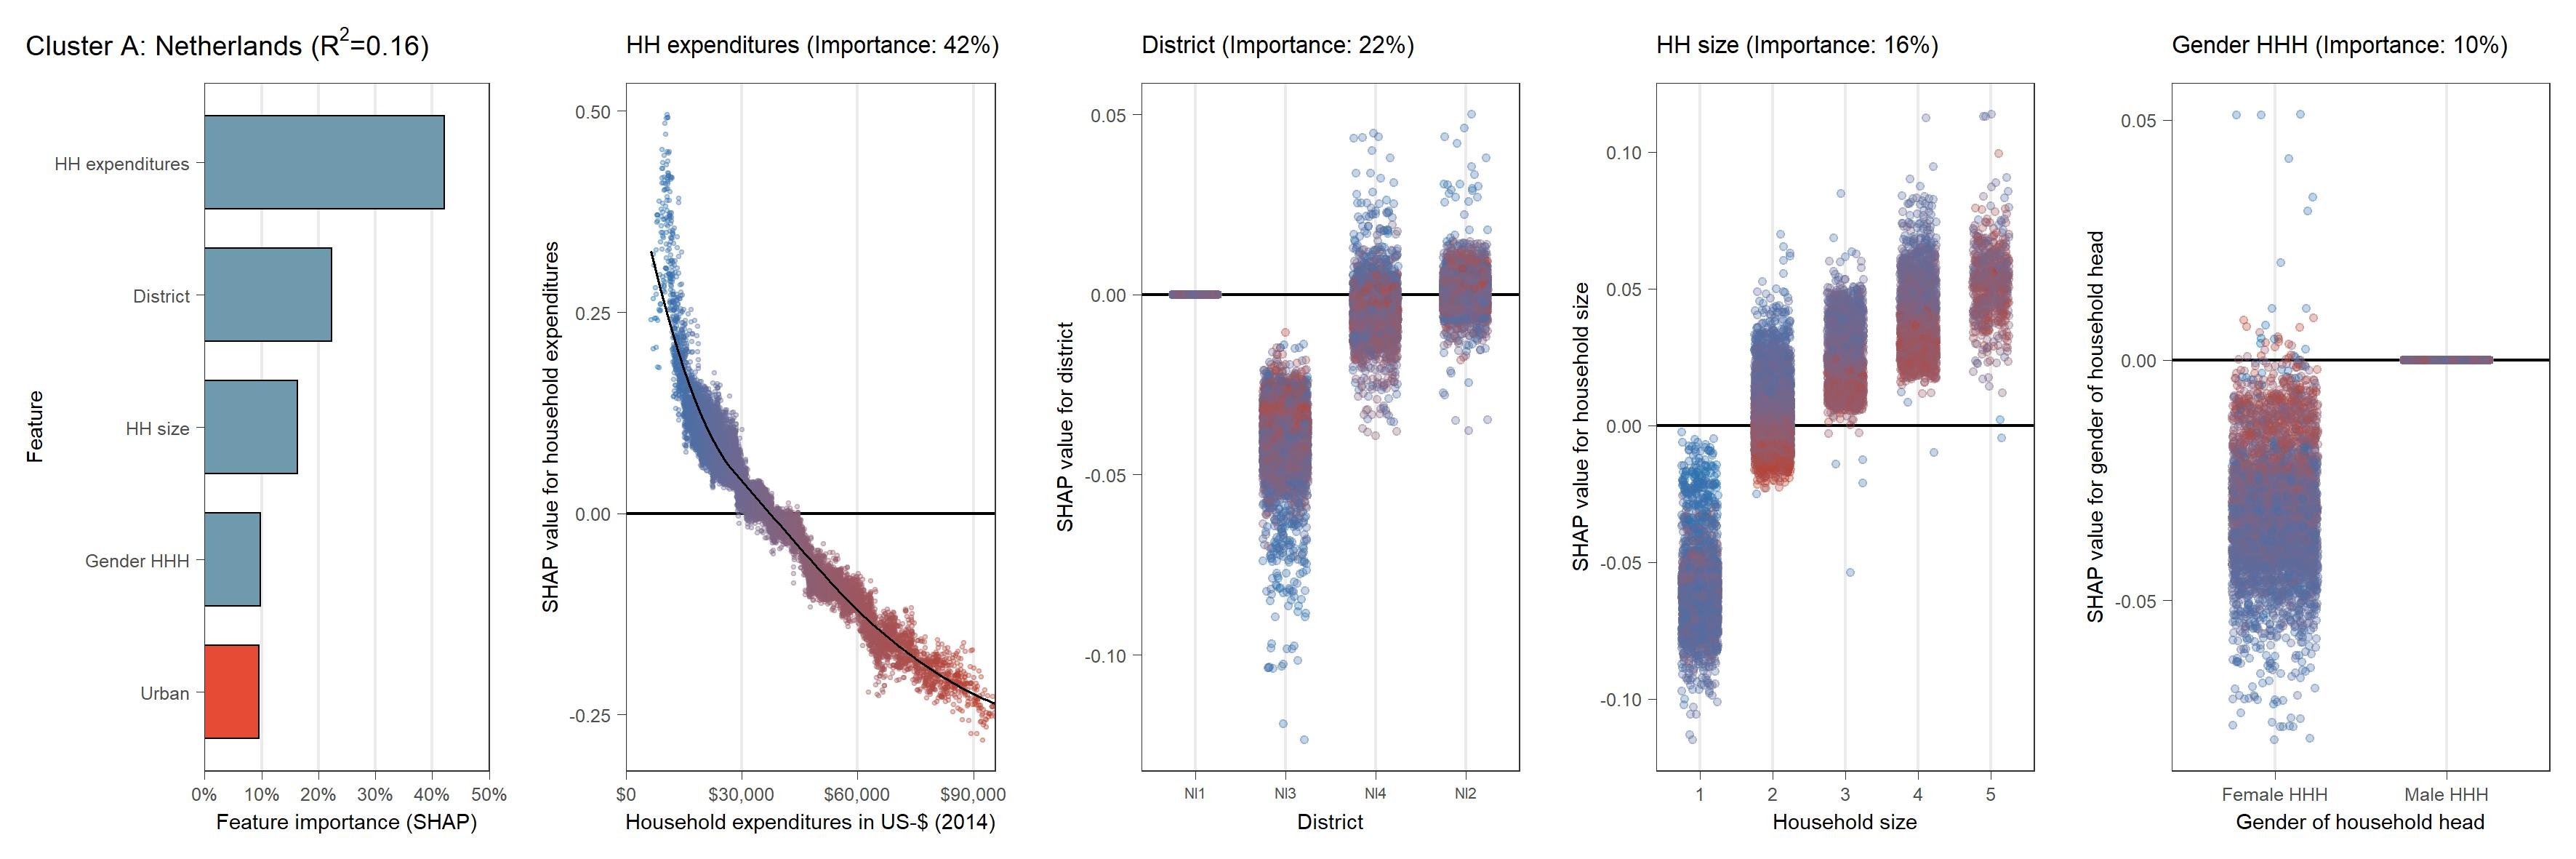
\includegraphics[width=\textwidth]{Figure 5b/Figure_5b_NLD}     
         \end{subfigure}
    \\
    \vspace{0.5cm}
    \begin{subcaption2}
     This figure shows SHAP-values for predicting carbon intensity over feature values for 87 countries in order of nine country-clusters and silhouette width. The bar chart displays normalized average absolute SHAP-values for all features. Features with less than 3\% of normalized SHAP-values are subsumed as "Other features (Sum)". Charts show SHAP-values over total household expenditures for all countries and for the three most important features in each country besides total household expenditures. Colors represent household expenditures with blue (red) colors indicating lower (higher) household expenditures.
     \end{subcaption2}
\end{figure}

\begin{figure}[ht!]\ContinuedFloat
    \centering
   \begin{subfigure}[b]{\textwidth}
   \centering
         \caption{Partial dependence plot (SHAP) for Norway (cluster A)}
         \label{fig:5b_NOR}
         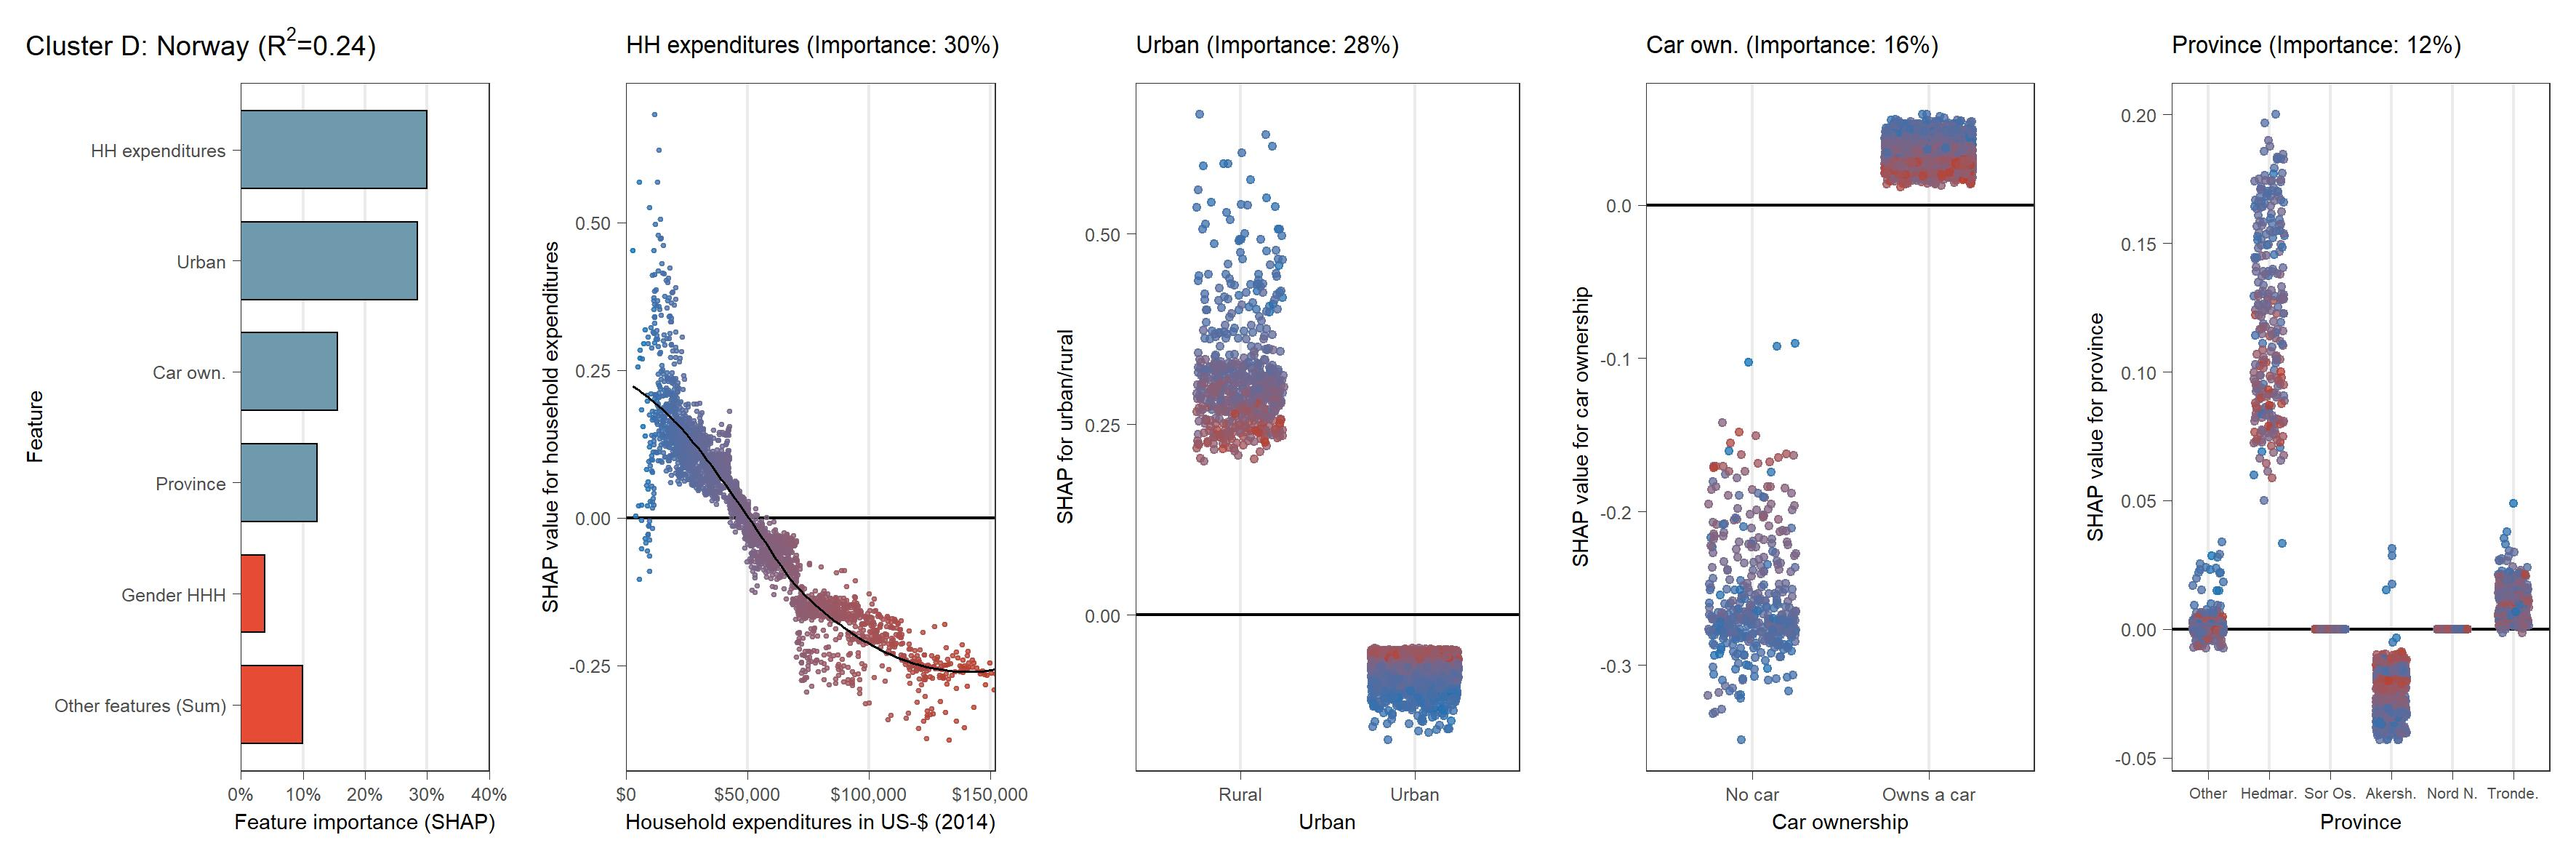
\includegraphics[width=\textwidth]{Figure 5b/Figure_5b_NOR}
         \end{subfigure}
    \\
    \vspace{0.5cm}
   \begin{subfigure}[b]{\textwidth}         
         \centering
         \caption{Partial dependence plot (SHAP) for Poland (cluster A)}
         \label{fig:5b_POL}
         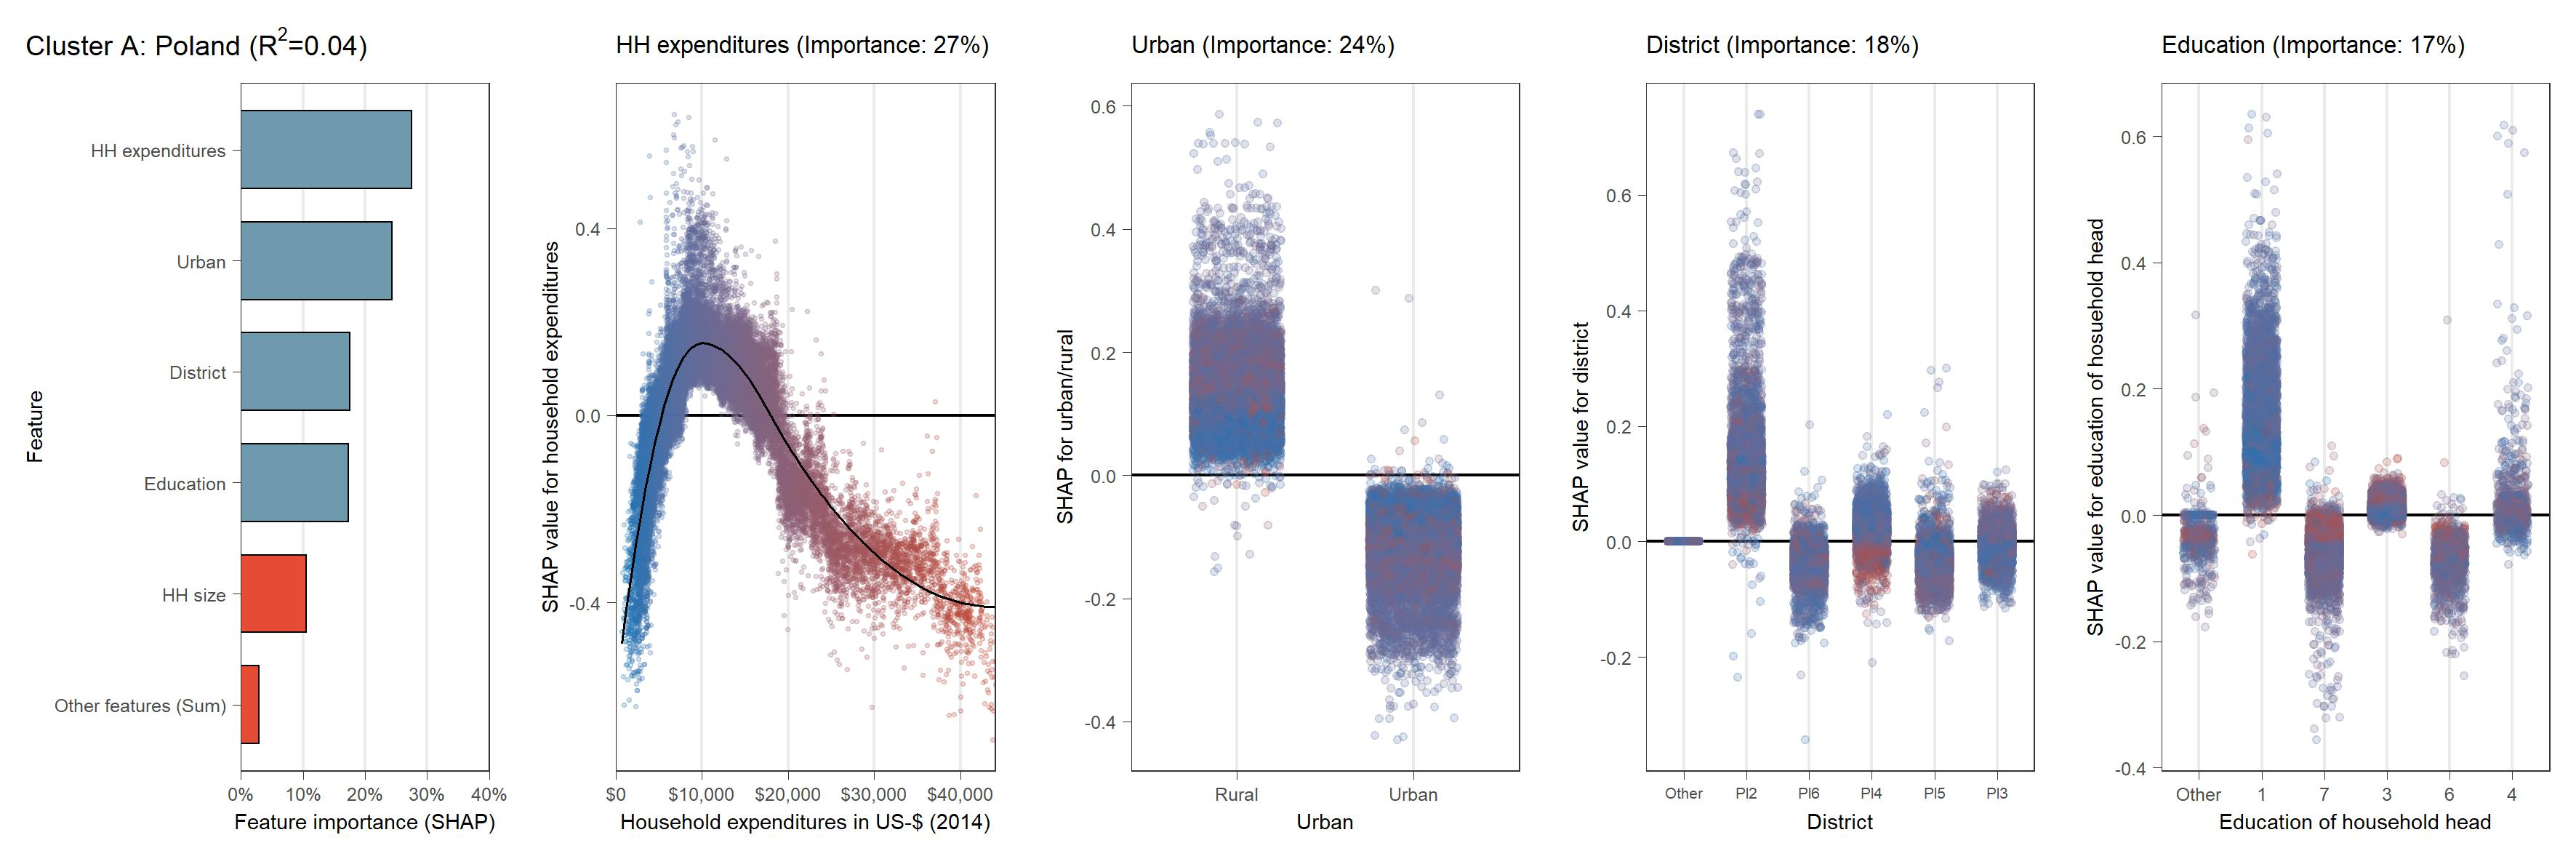
\includegraphics[width=\textwidth]{Figure 5b/Figure_5b_POL}
         \end{subfigure}
    \\
    \vspace{0.5cm}
   \begin{subfigure}[b]{\textwidth}
   \centering
         \caption{Partial dependence plot (SHAP) for Portugal (cluster A)}
         \label{fig:5b_PRT}
         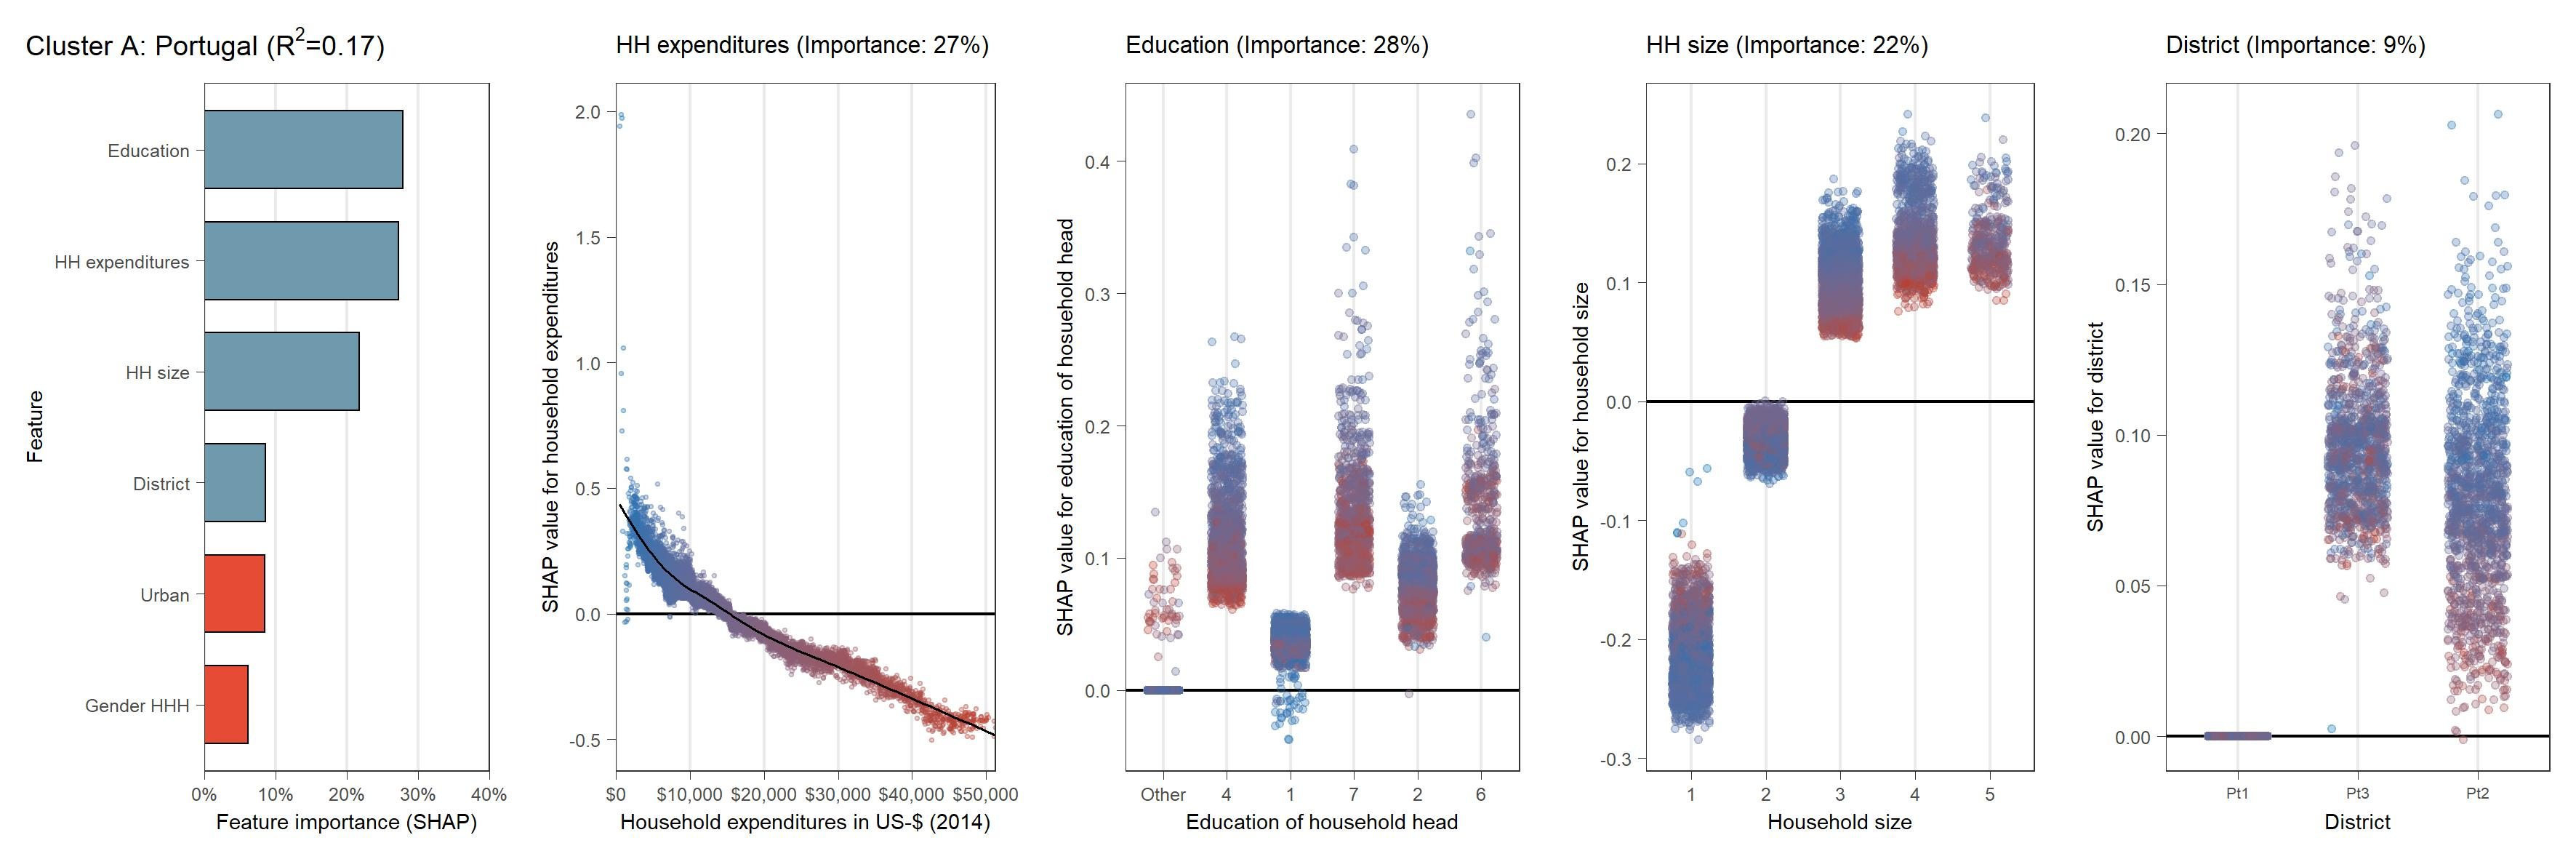
\includegraphics[width=\textwidth]{Figure 5b/Figure_5b_PRT}
         \end{subfigure}
    \\
    \vspace{0.5cm}
    \begin{subcaption2}
     This figure shows SHAP-values for predicting carbon intensity over feature values for 87 countries in order of nine country-clusters and silhouette width. The bar chart displays normalized average absolute SHAP-values for all features. Features with less than 3\% of normalized SHAP-values are subsumed as "Other features (Sum)". Charts show SHAP-values over total household expenditures for all countries and for the three most important features in each country besides total household expenditures. Colors represent household expenditures with blue (red) colors indicating lower (higher) household expenditures.
     \end{subcaption2}
\end{figure}

\begin{figure}[ht!]\ContinuedFloat
    \centering
   \begin{subfigure}[b]{\textwidth}
    \centering
         \caption{Partial dependence plot (SHAP) for Romania (cluster A)}
         \label{fig:5b_ROU}
         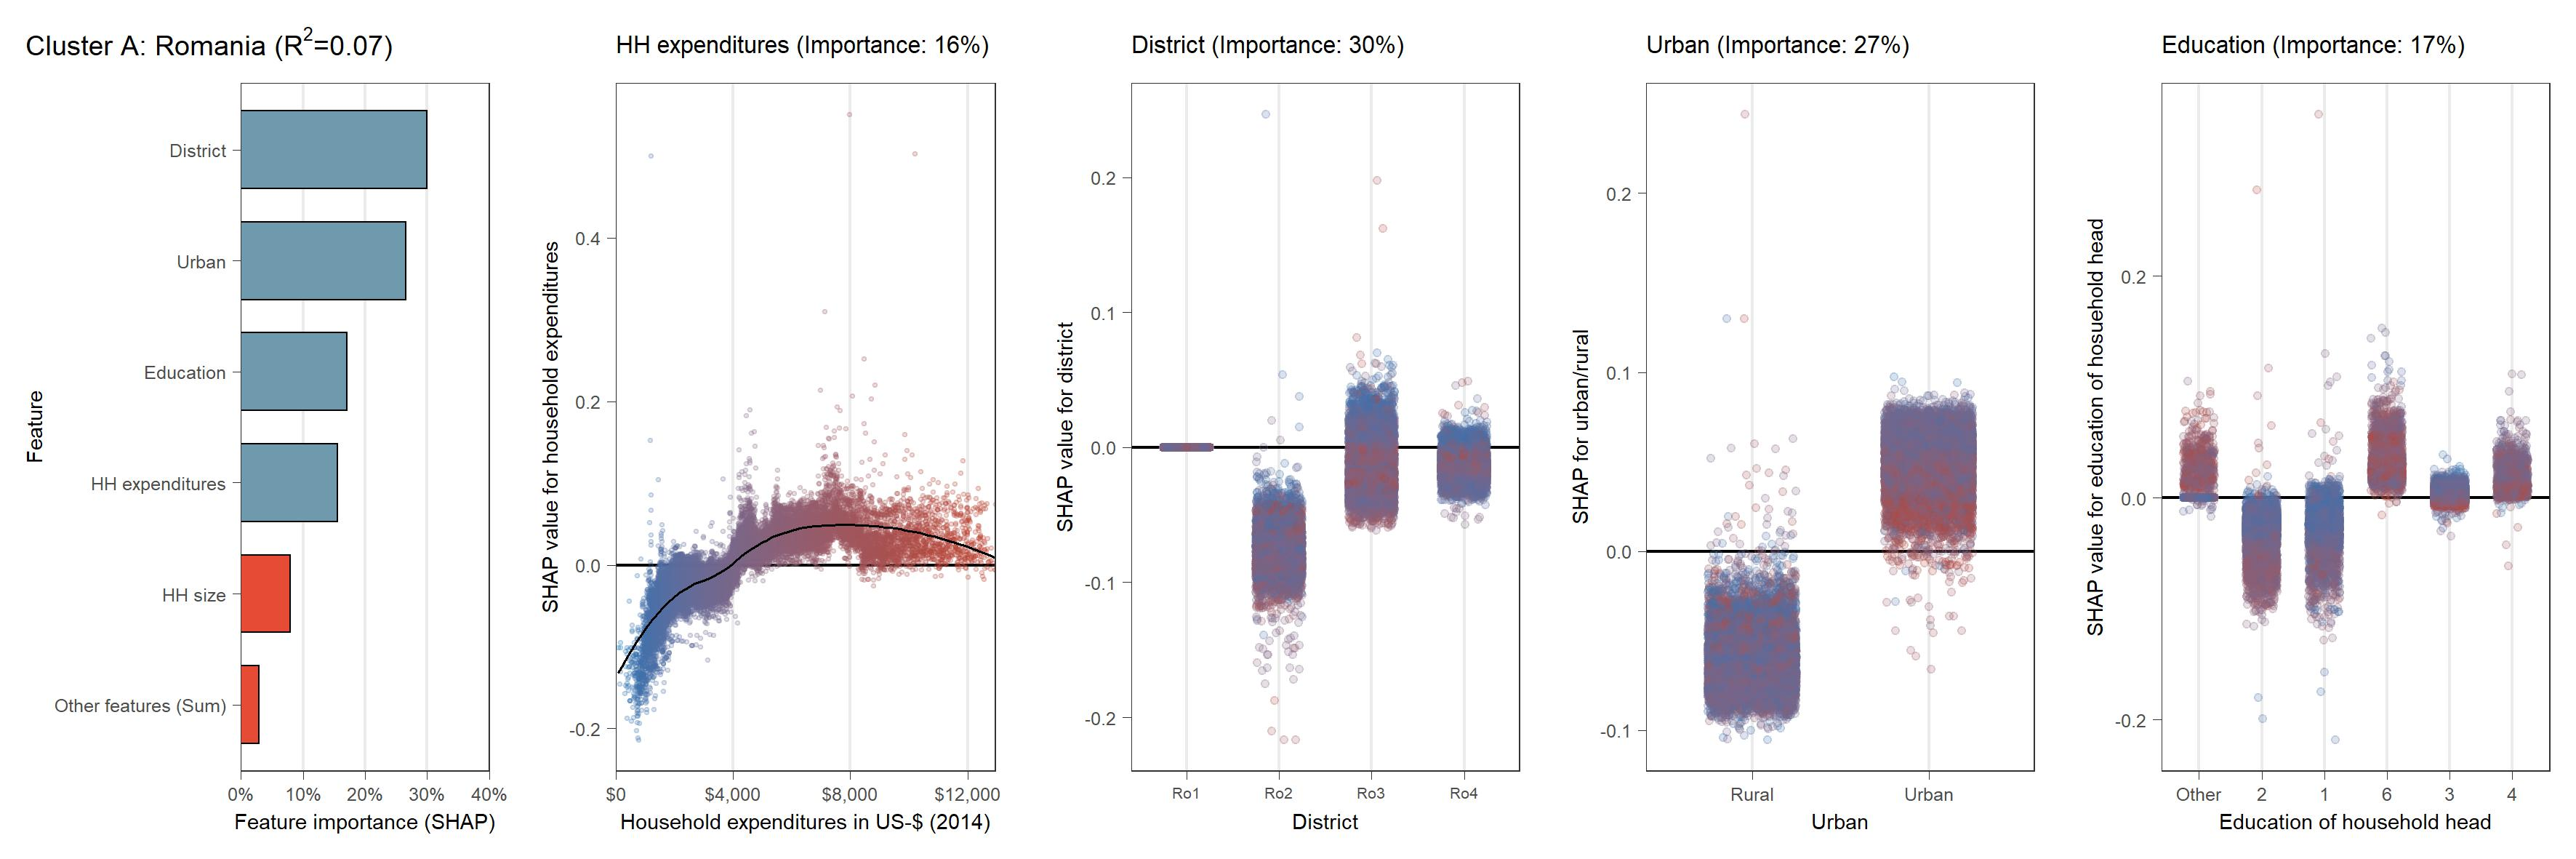
\includegraphics[width=\textwidth]{Figure 5b/Figure_5b_ROU}
         \end{subfigure}
    \\
    \vspace{0.5cm}
   \begin{subfigure}[b]{\textwidth}
   \centering
         \caption{Partial dependence plot (SHAP) for Serbia (cluster A)}
         \label{fig:5b_SRB}
         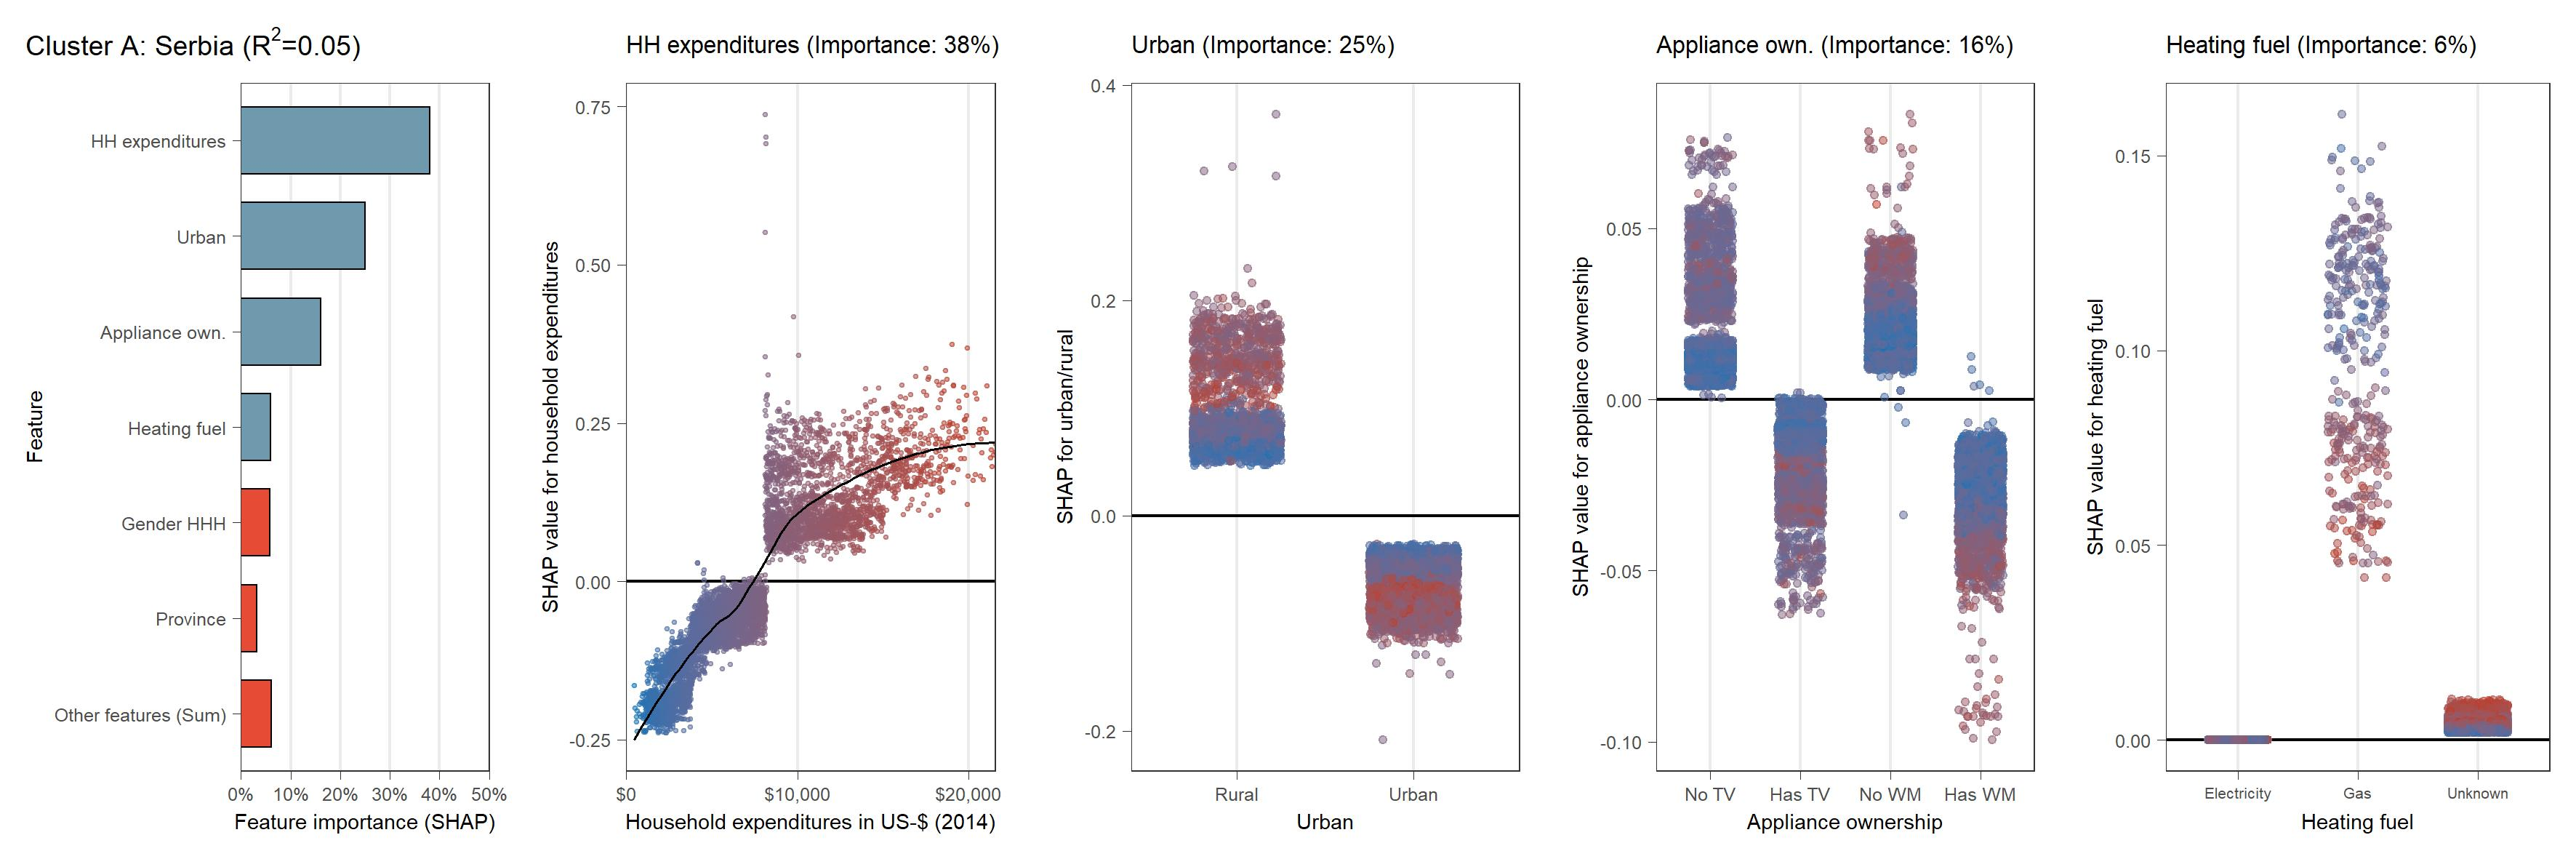
\includegraphics[width=\textwidth]{Figure 5b/Figure_5b_SRB} 
         \end{subfigure}
    \\
    \vspace{0.5cm}
   \begin{subfigure}[b]{\textwidth}
   \centering
         \caption{Partial dependence plot (SHAP) for Suriname (cluster A)}
         \label{fig:5b_SUR}
         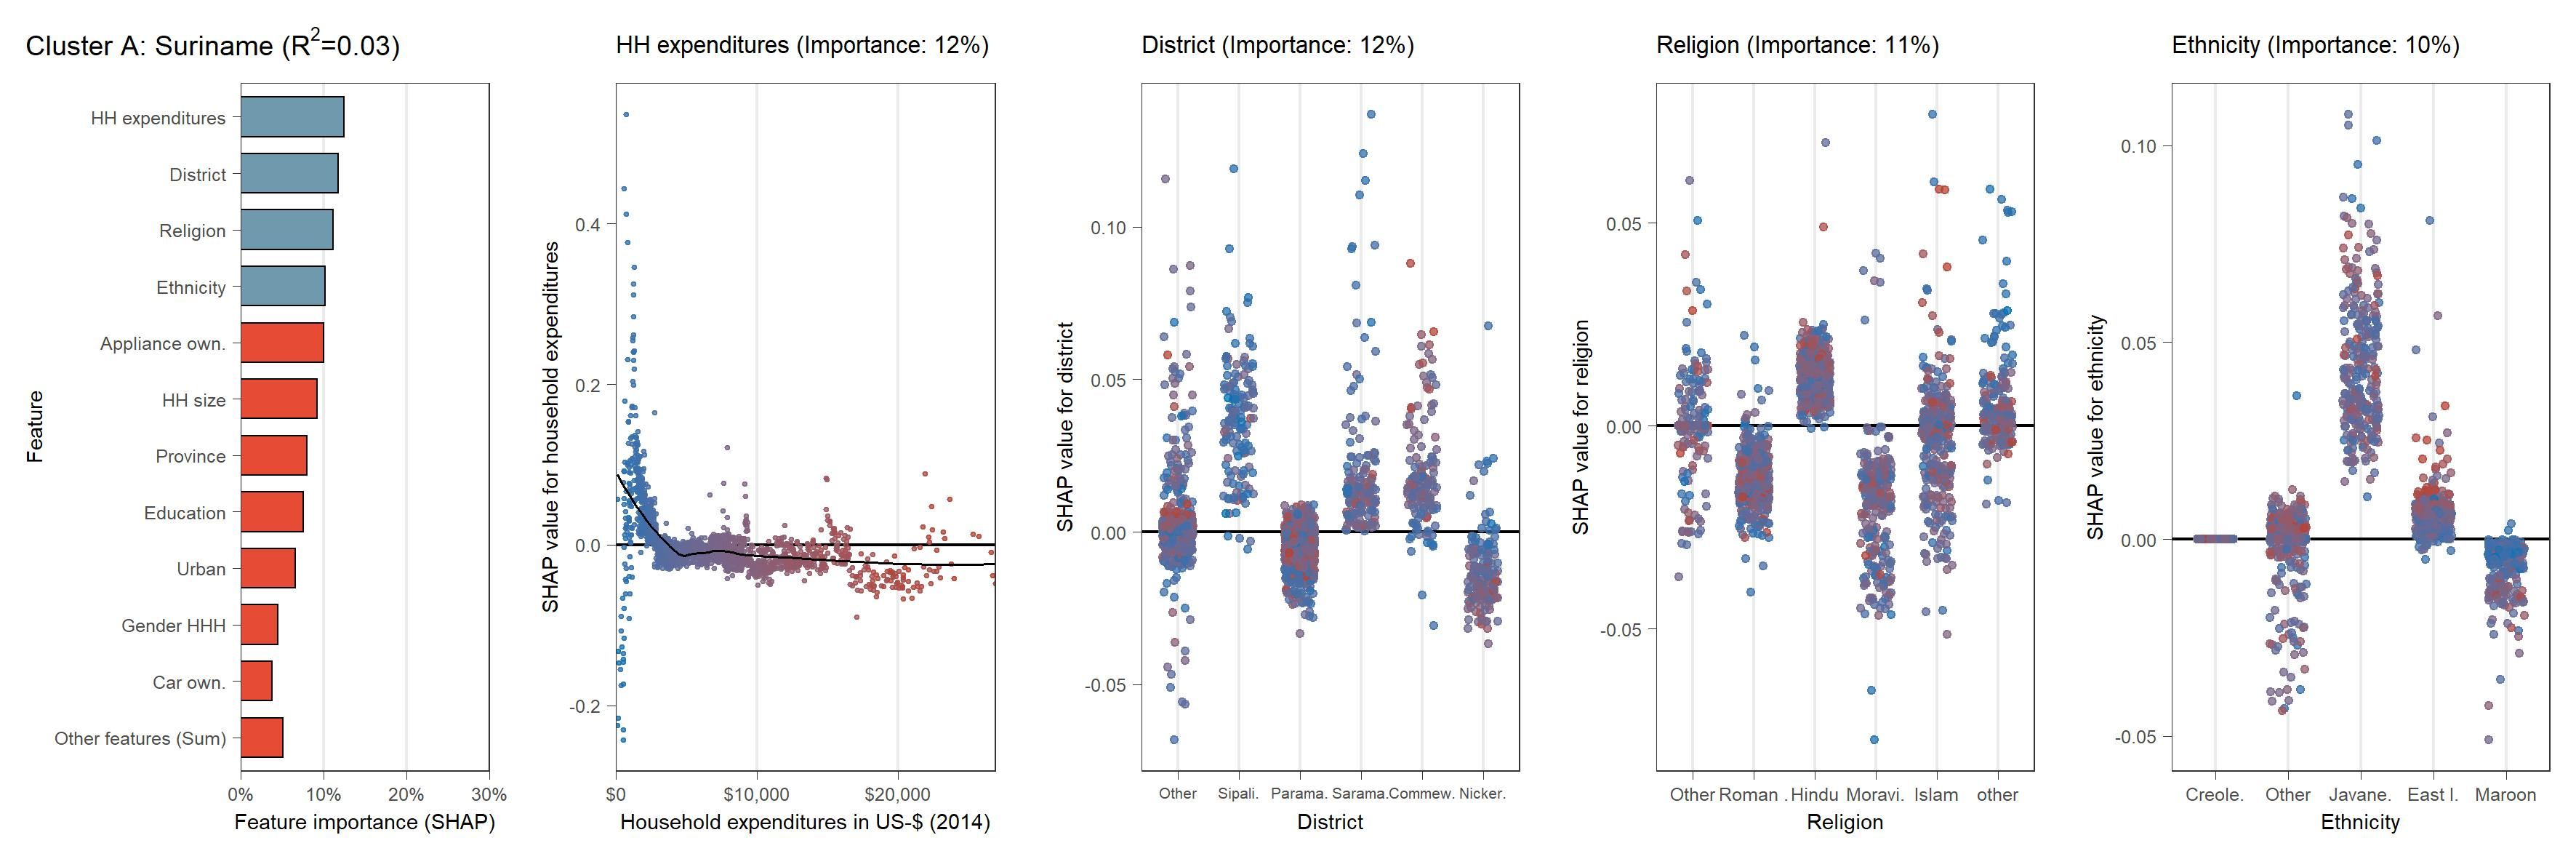
\includegraphics[width=\textwidth]{Figure 5b/Figure_5b_SUR}         
     \end{subfigure}
    \\
    \vspace{0.5cm}
    \begin{subcaption2}
     This figure shows SHAP-values for predicting carbon intensity over feature values for 87 countries in order of nine country-clusters and silhouette width. The bar chart displays normalized average absolute SHAP-values for all features. Features with less than 3\% of normalized SHAP-values are subsumed as "Other features (Sum)". Charts show SHAP-values over total household expenditures for all countries and for the three most important features in each country besides total household expenditures. Colors represent household expenditures with blue (red) colors indicating lower (higher) household expenditures.
     \end{subcaption2}
\end{figure}

\begin{figure}[ht!]\ContinuedFloat
    \centering
   \begin{subfigure}[b]{\textwidth}
   \centering
         \caption{Partial dependence plot (SHAP) for Slovakia (cluster A)}
         \label{fig:5b_SVK}
         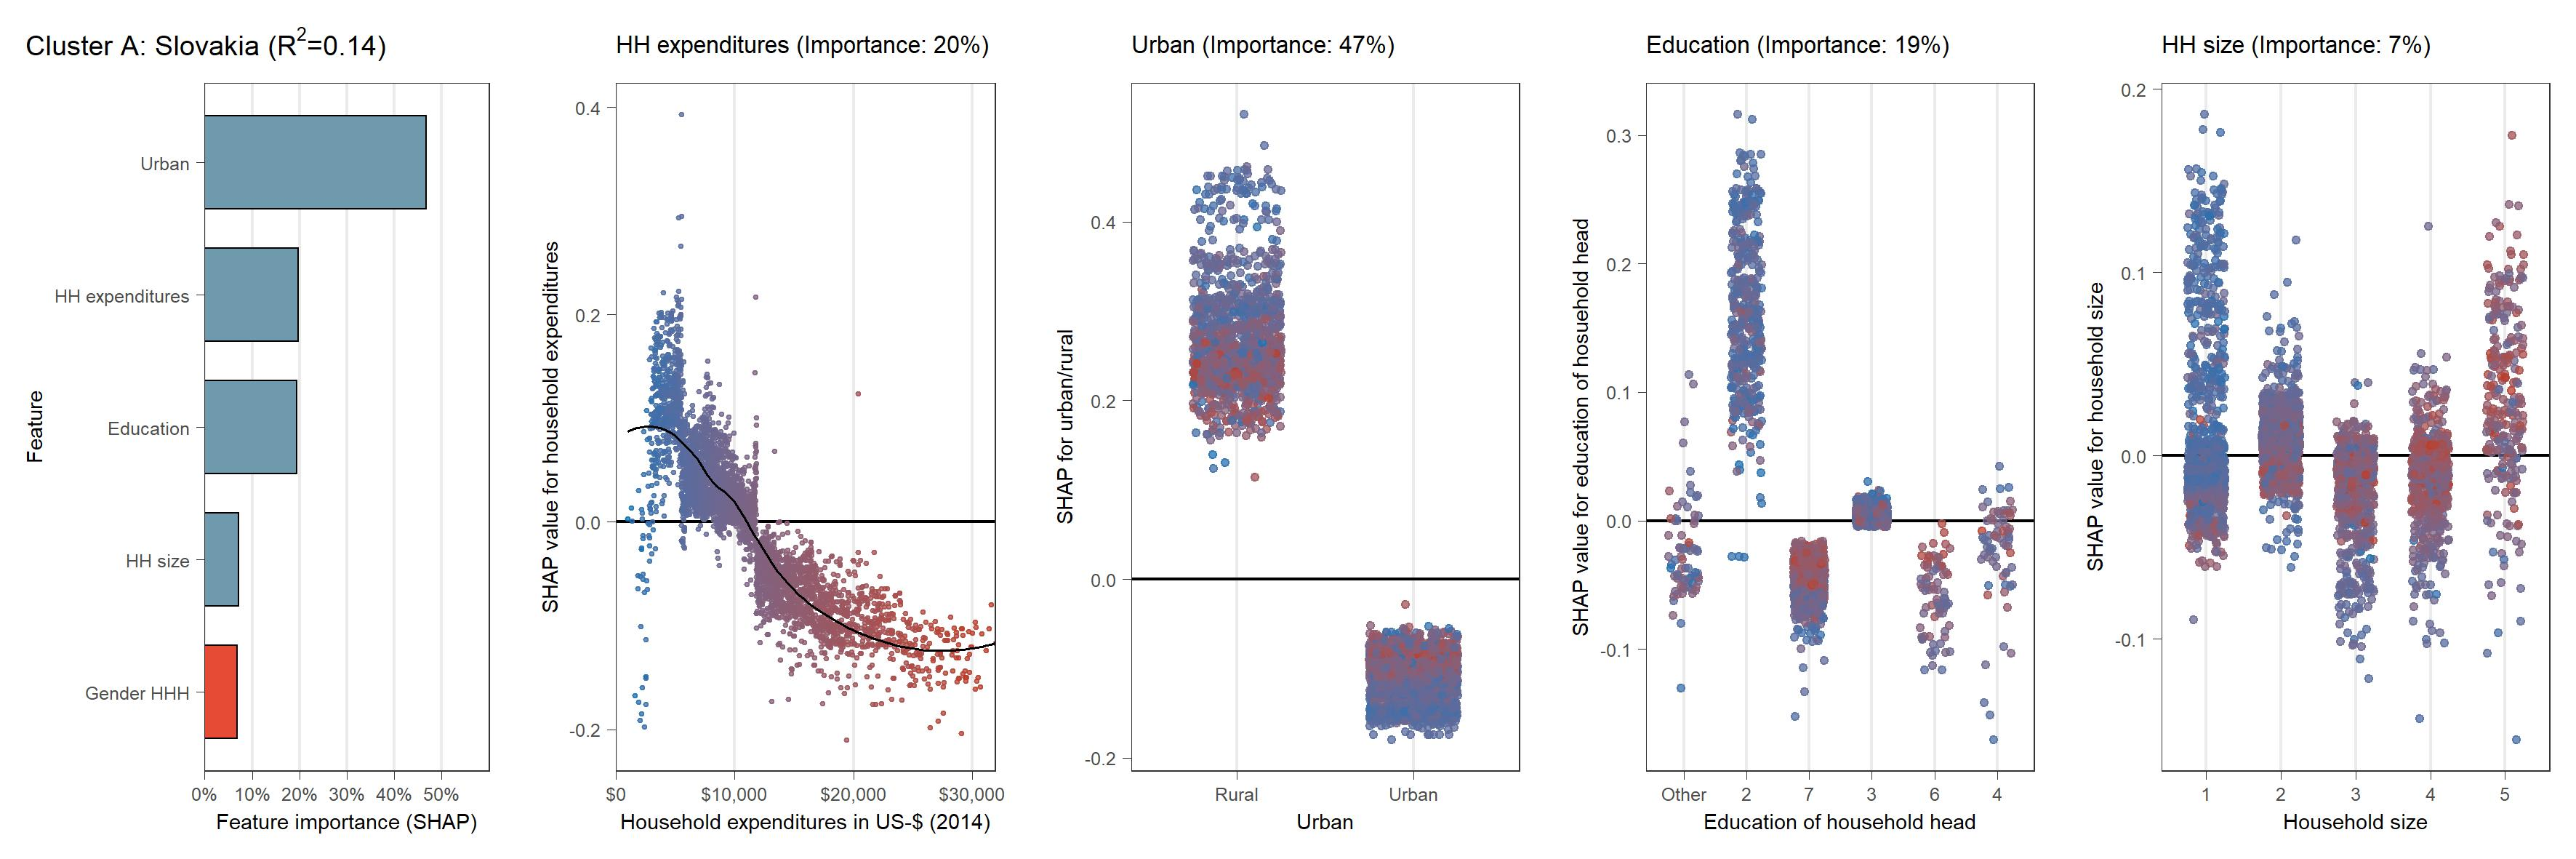
\includegraphics[width=\textwidth]{Figure 5b/Figure_5b_SVK}
         \end{subfigure}
    \\
    \vspace{0.5cm}
   \begin{subfigure}[b]{\textwidth}
         \centering
         \caption{Partial dependence plot (SHAP) for Sweden (cluster A)}
         \label{fig:5b_SWE}
         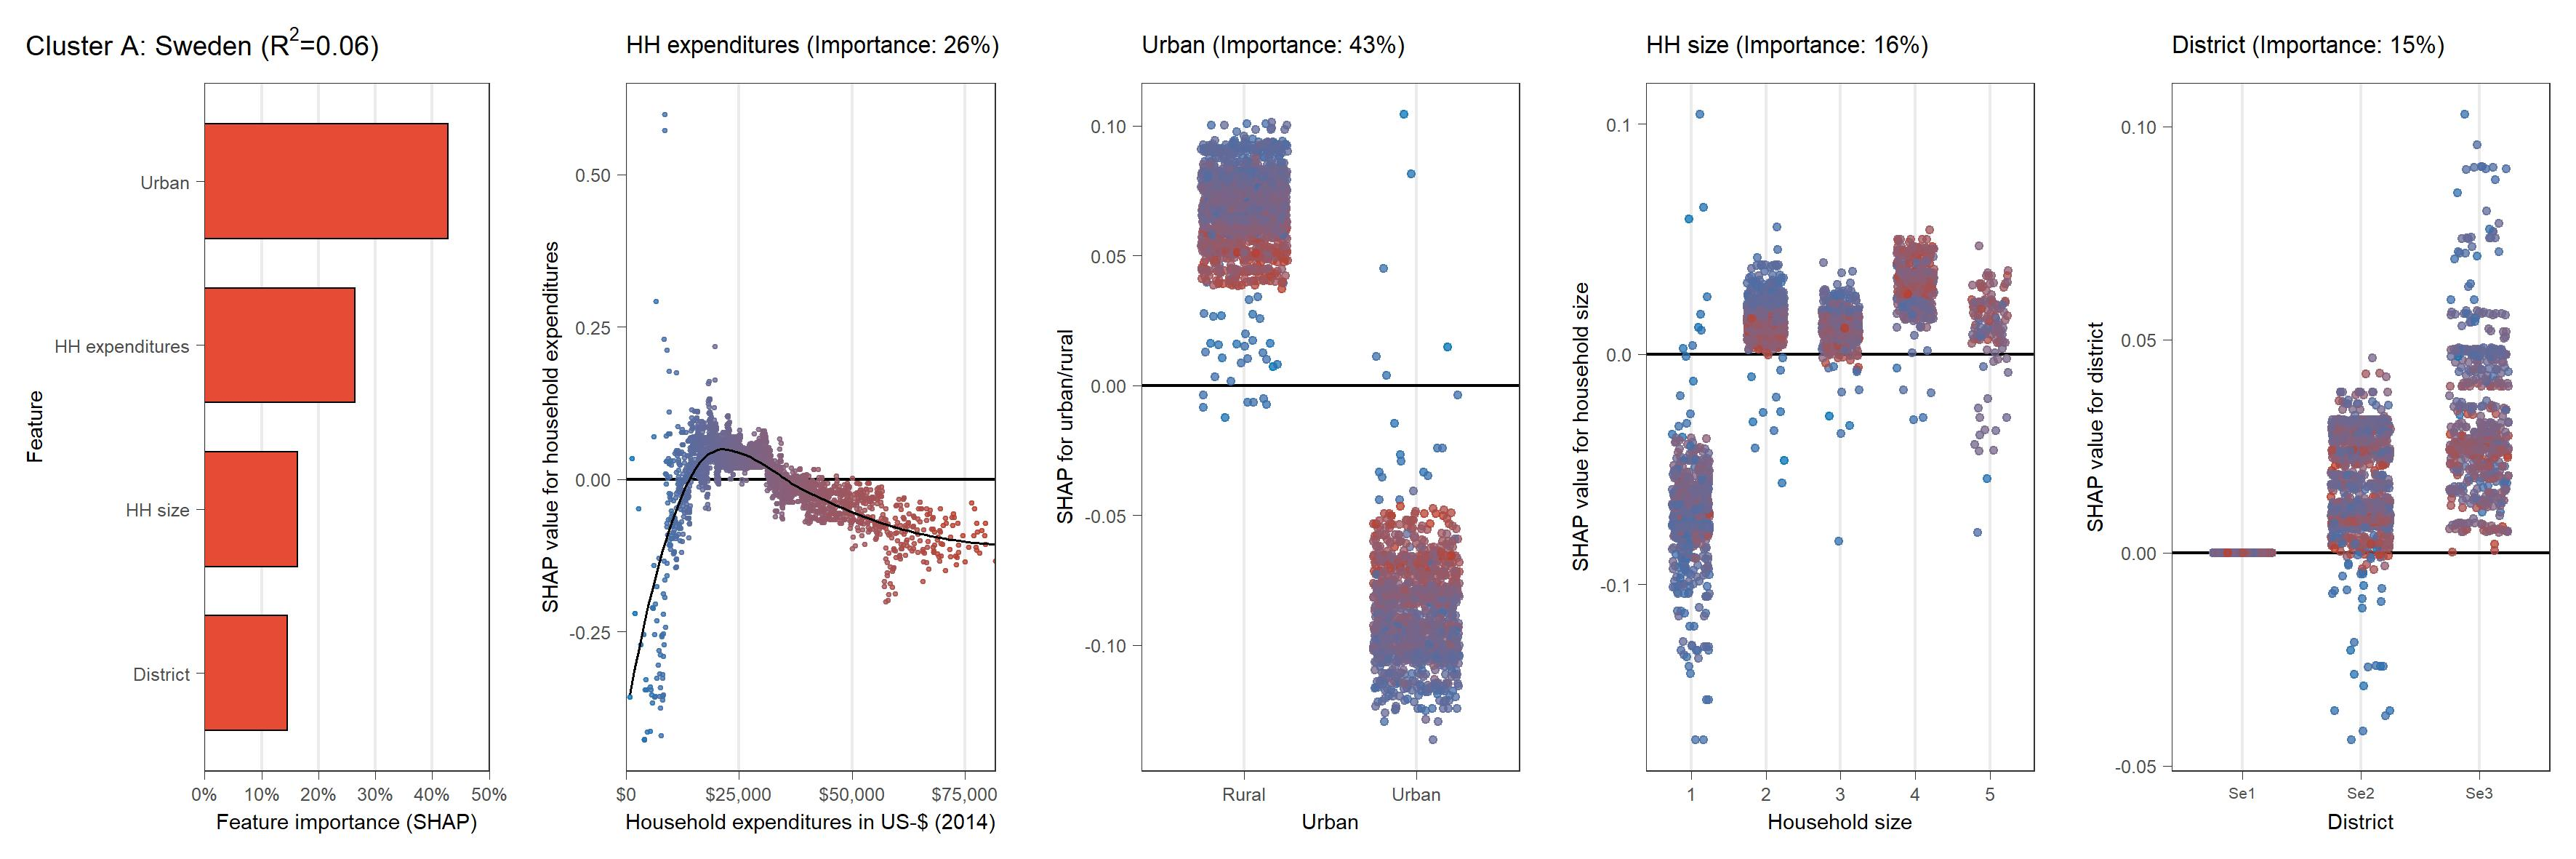
\includegraphics[width=\textwidth]{Figure 5b/Figure_5b_SWE}
         \end{subfigure}
    \\
    \vspace{0.5cm}
   \begin{subfigure}[b]{\textwidth}
    \centering
         \caption{Partial dependence plot (SHAP) for Uruguay (cluster A)}
         \label{fig:5b_URY}
         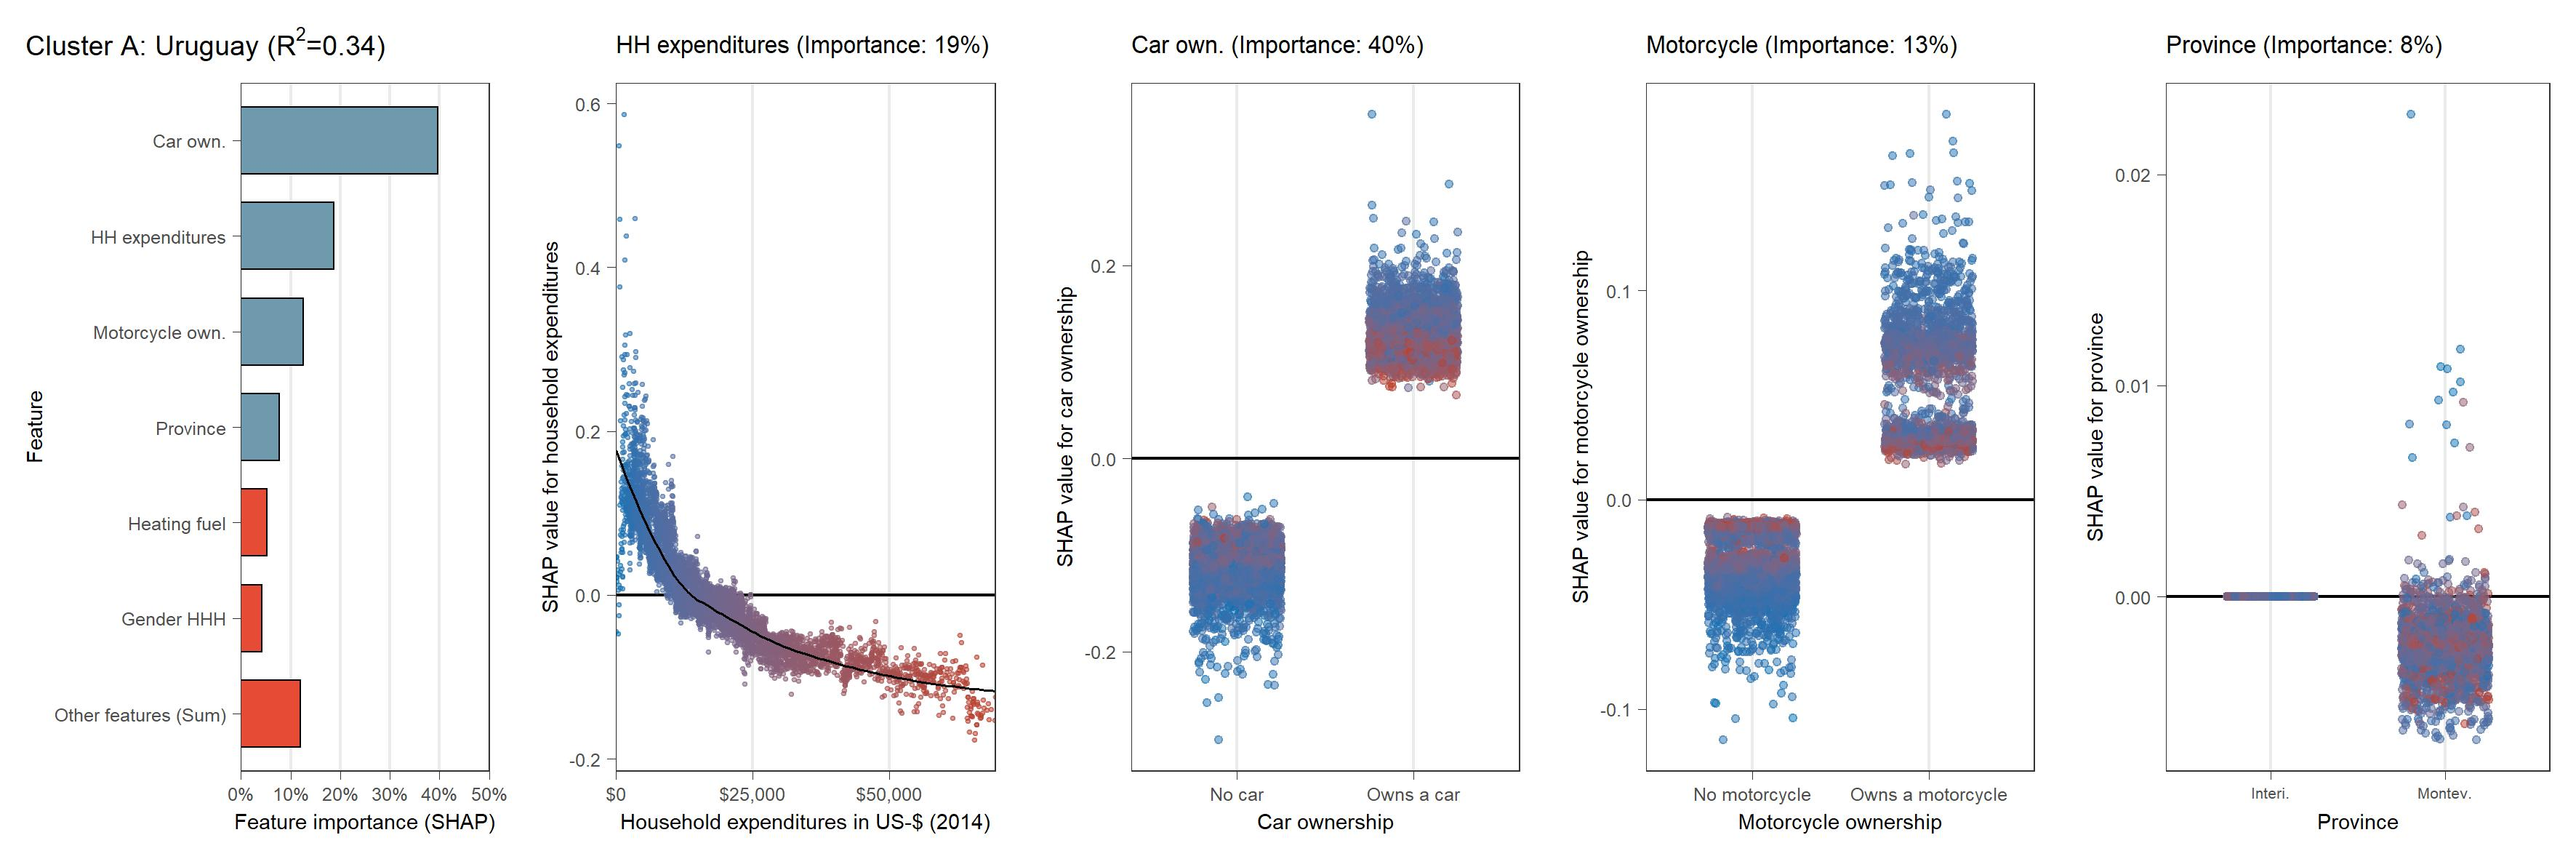
\includegraphics[width=\textwidth]{Figure 5b/Figure_5b_URY}
         \end{subfigure}
    \\
    \vspace{0.5cm}
    \begin{subcaption2}
     This figure shows SHAP-values for predicting carbon intensity over feature values for 87 countries in order of nine country-clusters and silhouette width. The bar chart displays normalized average absolute SHAP-values for all features. Features with less than 3\% of normalized SHAP-values are subsumed as "Other features (Sum)". Charts show SHAP-values over total household expenditures for all countries and for the three most important features in each country besides total household expenditures. Colors represent household expenditures with blue (red) colors indicating lower (higher) household expenditures.
     \end{subcaption2}
\end{figure}

\begin{figure}[ht!]\ContinuedFloat
    \centering
   \begin{subfigure}[b]{\textwidth}
   \centering
         \caption{Partial dependence plot (SHAP) for USA (cluster A)}
         \label{fig:5b_USA}
         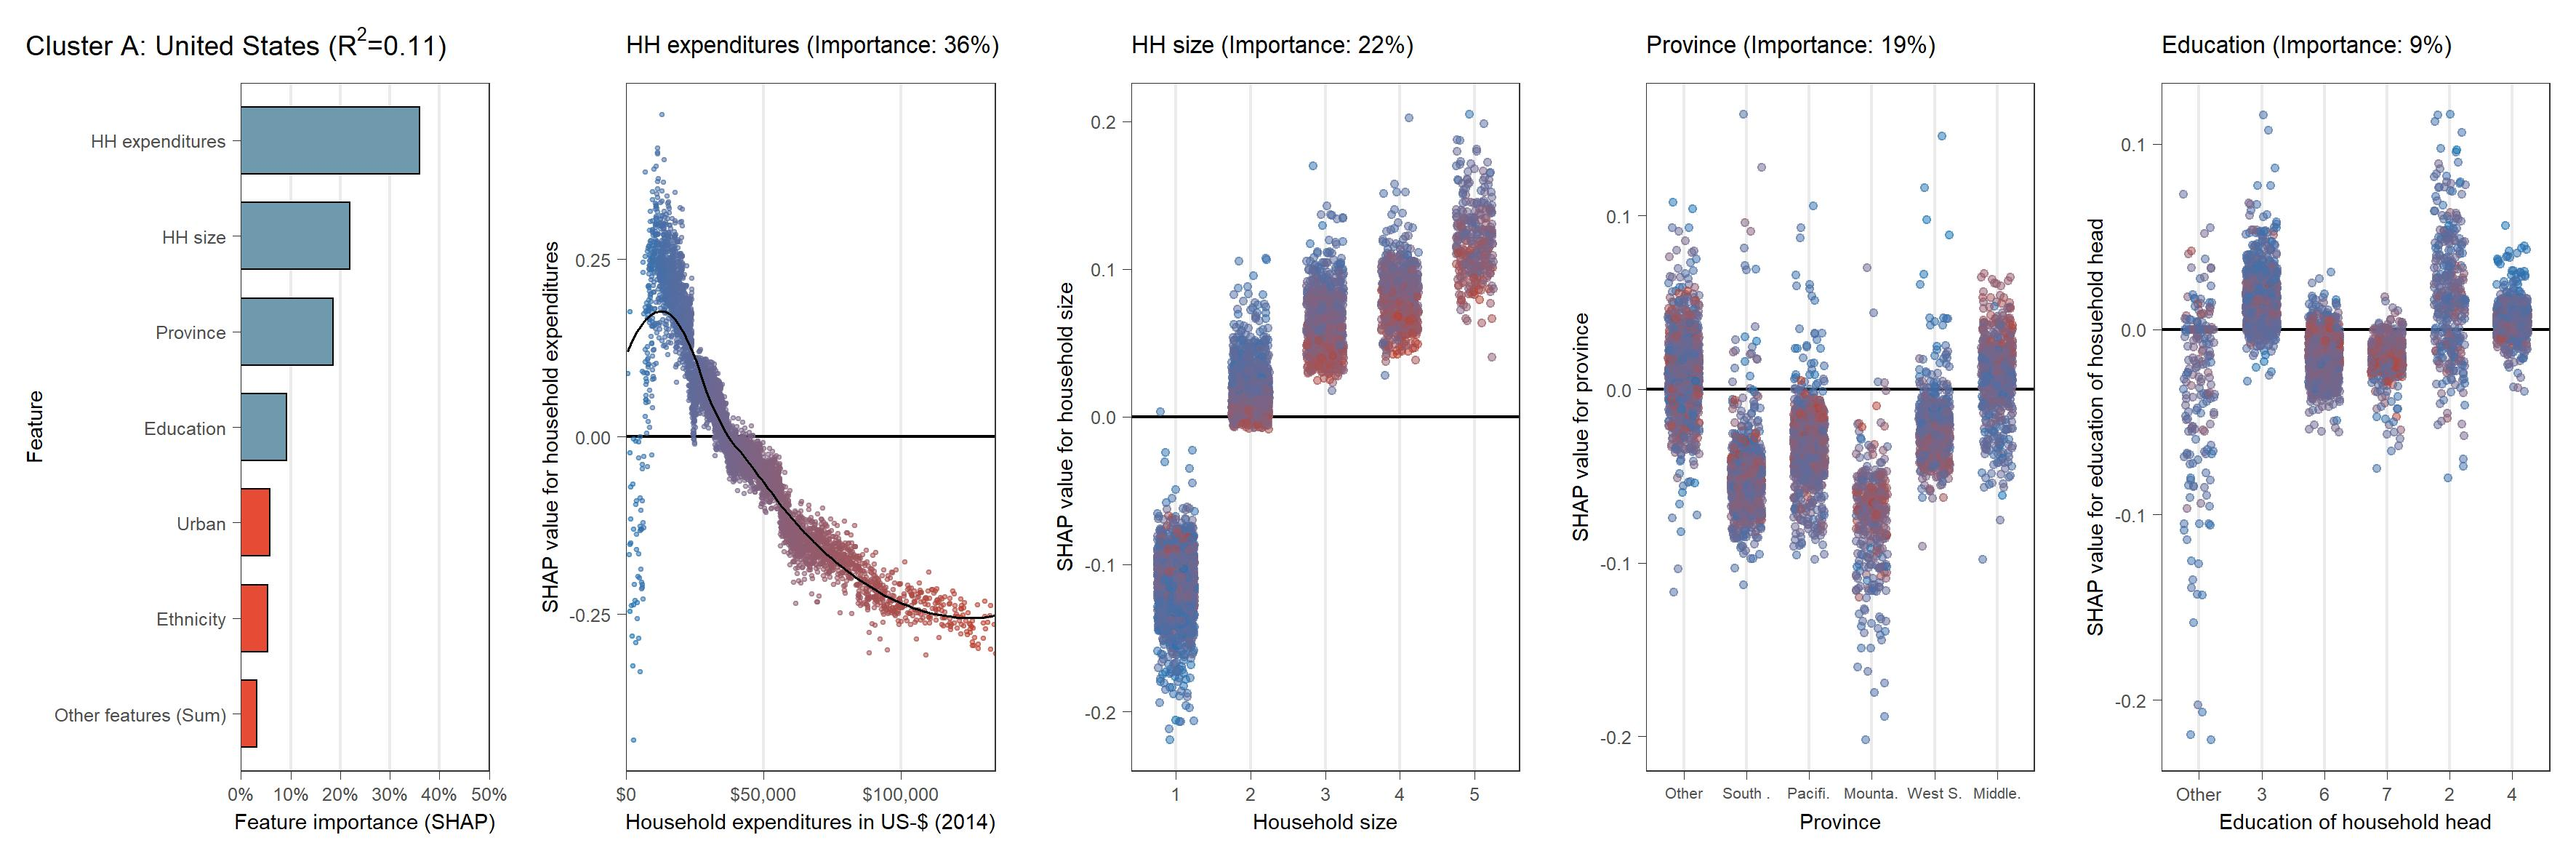
\includegraphics[width=\textwidth]{Figure 5b/Figure_5b_USA}   
         \end{subfigure}
    \\
    \vspace{0.5cm}
   \begin{subfigure}[b]{\textwidth}
         \centering
         \caption{Partial dependence plot (SHAP) for Benin (cluster B)}
         \label{fig:5b_BEN}
         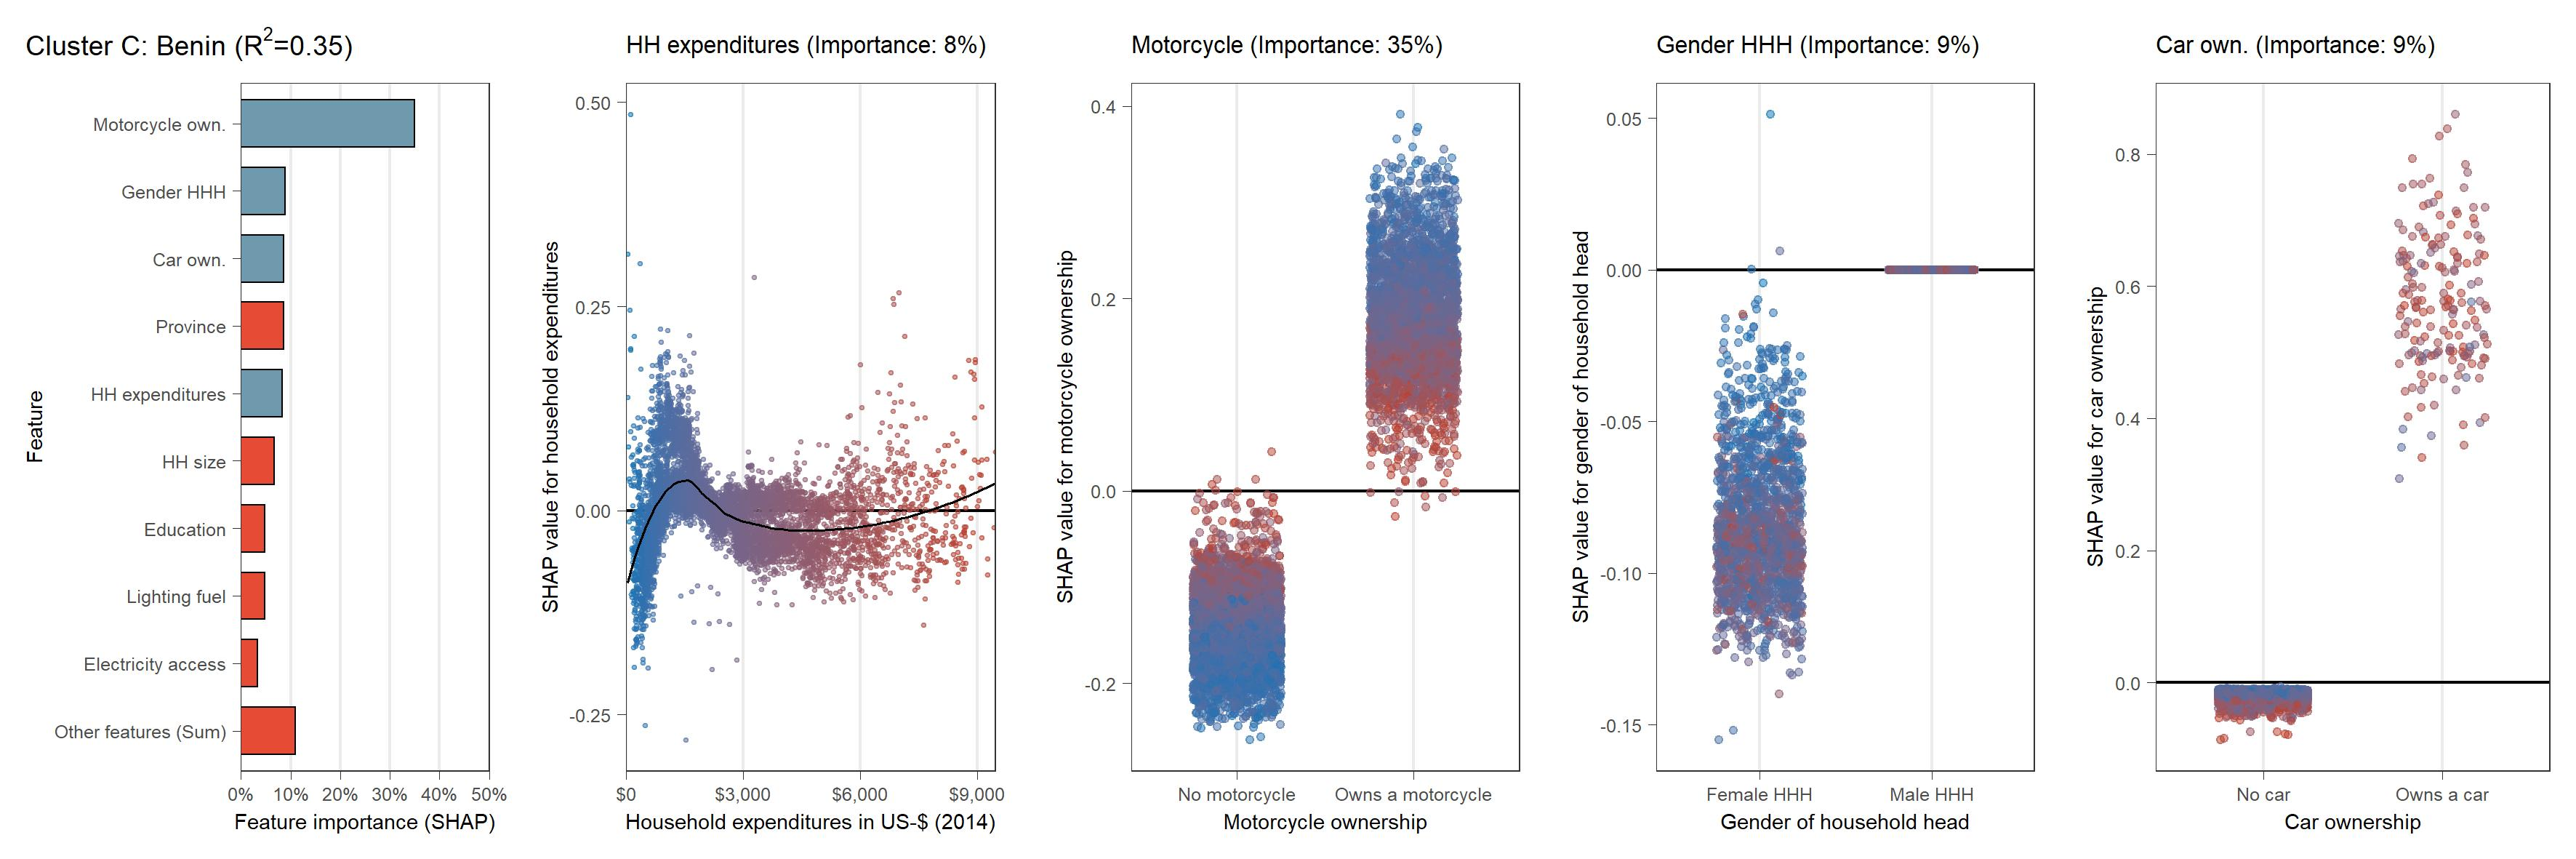
\includegraphics[width=\textwidth]{Figure 5b/Figure_5b_BEN}
         \end{subfigure}
    \\
    \vspace{0.5cm}
   \begin{subfigure}[b]{\textwidth}
   \centering
         \caption{Partial dependence plot (SHAP) for Burkina Faso (cluster B)}
         \label{fig:5b_BFA}
         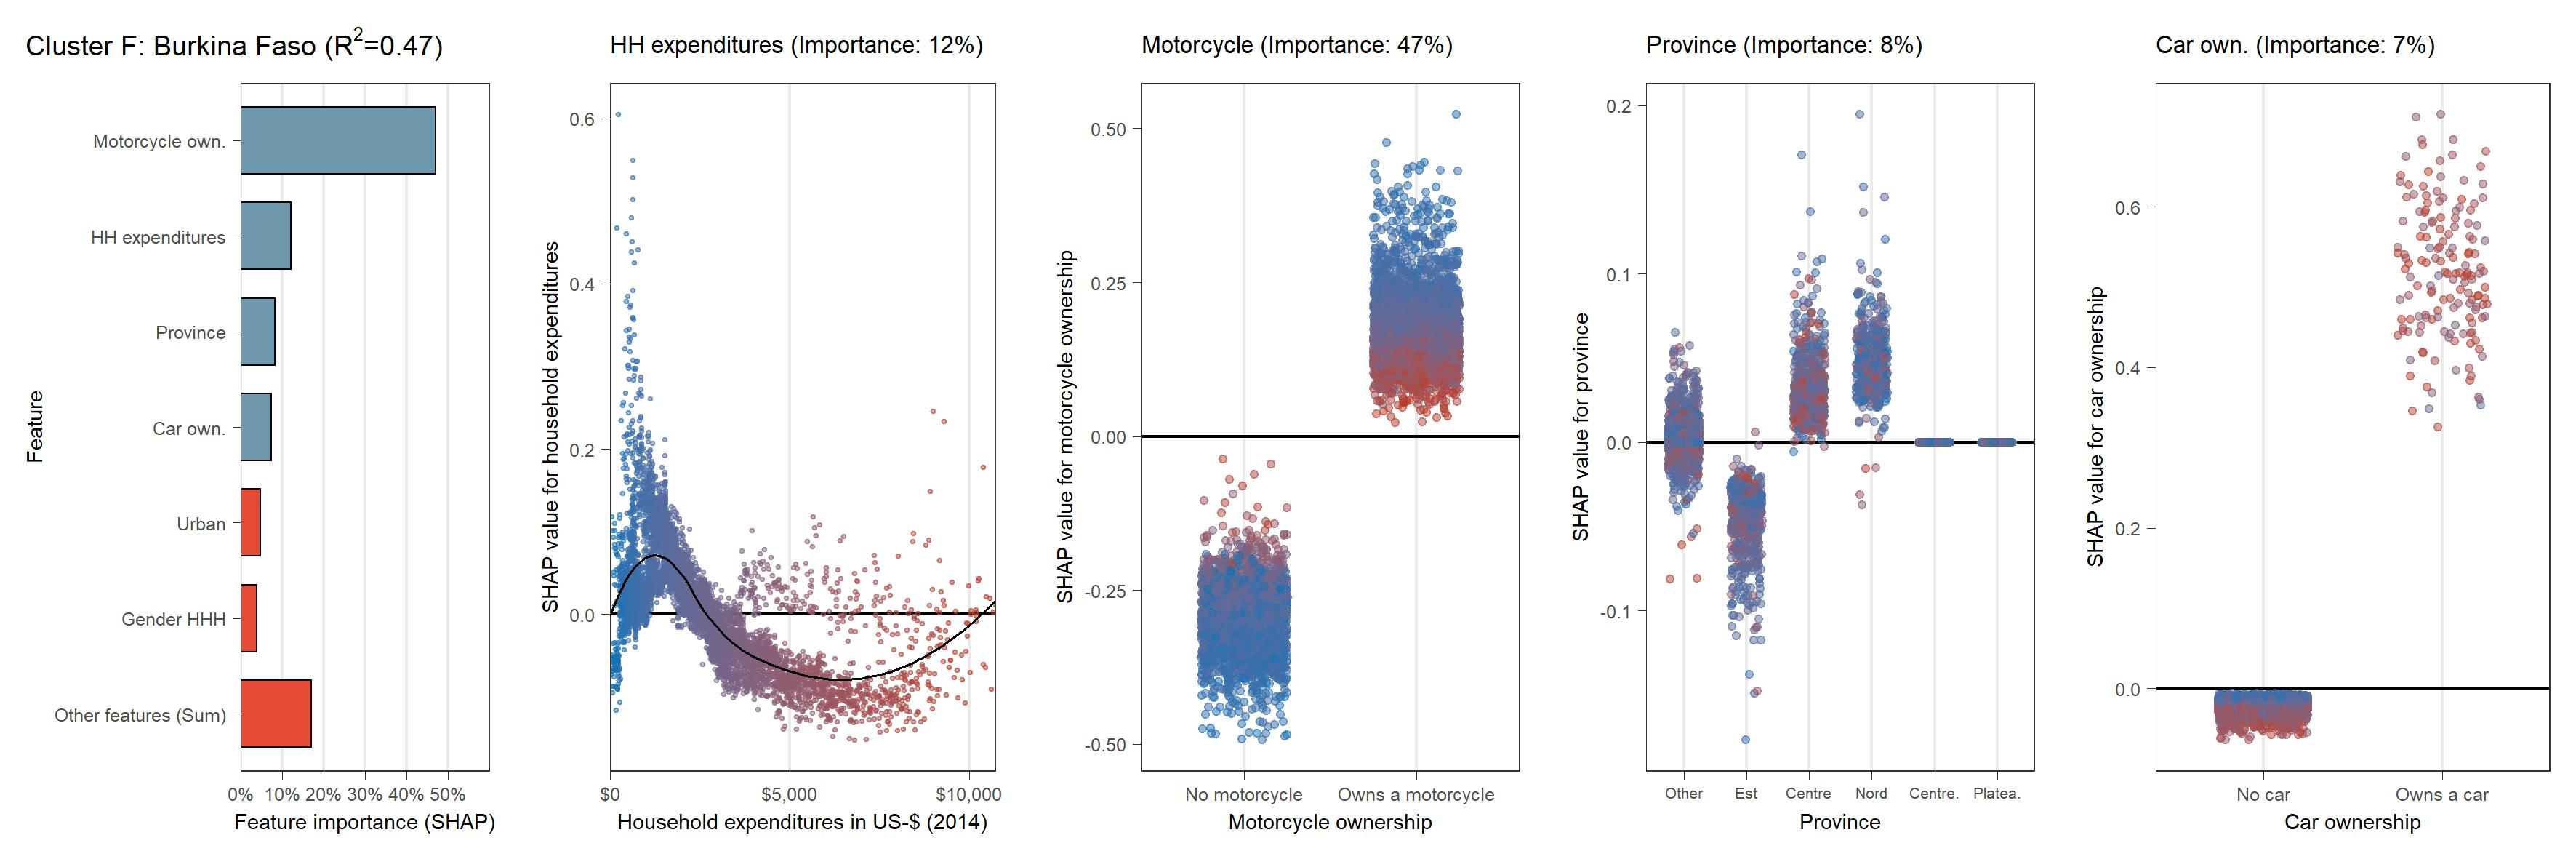
\includegraphics[width=\textwidth]{Figure 5b/Figure_5b_BFA}
    \end{subfigure}
    \\
    \vspace{0.5cm}
    \begin{subcaption2}
     This figure shows SHAP-values for predicting carbon intensity over feature values for 87 countries in order of nine country-clusters and silhouette width. The bar chart displays normalized average absolute SHAP-values for all features. Features with less than 3\% of normalized SHAP-values are subsumed as "Other features (Sum)". Charts show SHAP-values over total household expenditures for all countries and for the three most important features in each country besides total household expenditures. Colors represent household expenditures with blue (red) colors indicating lower (higher) household expenditures.
     \end{subcaption2}
\end{figure}

\begin{figure}[ht!]\ContinuedFloat
    \centering
   \begin{subfigure}[b]{\textwidth}
   \centering
         \caption{Partial dependence plot (SHAP) for Bangladesh (cluster B)}
         \label{fig:5b_BGD}
         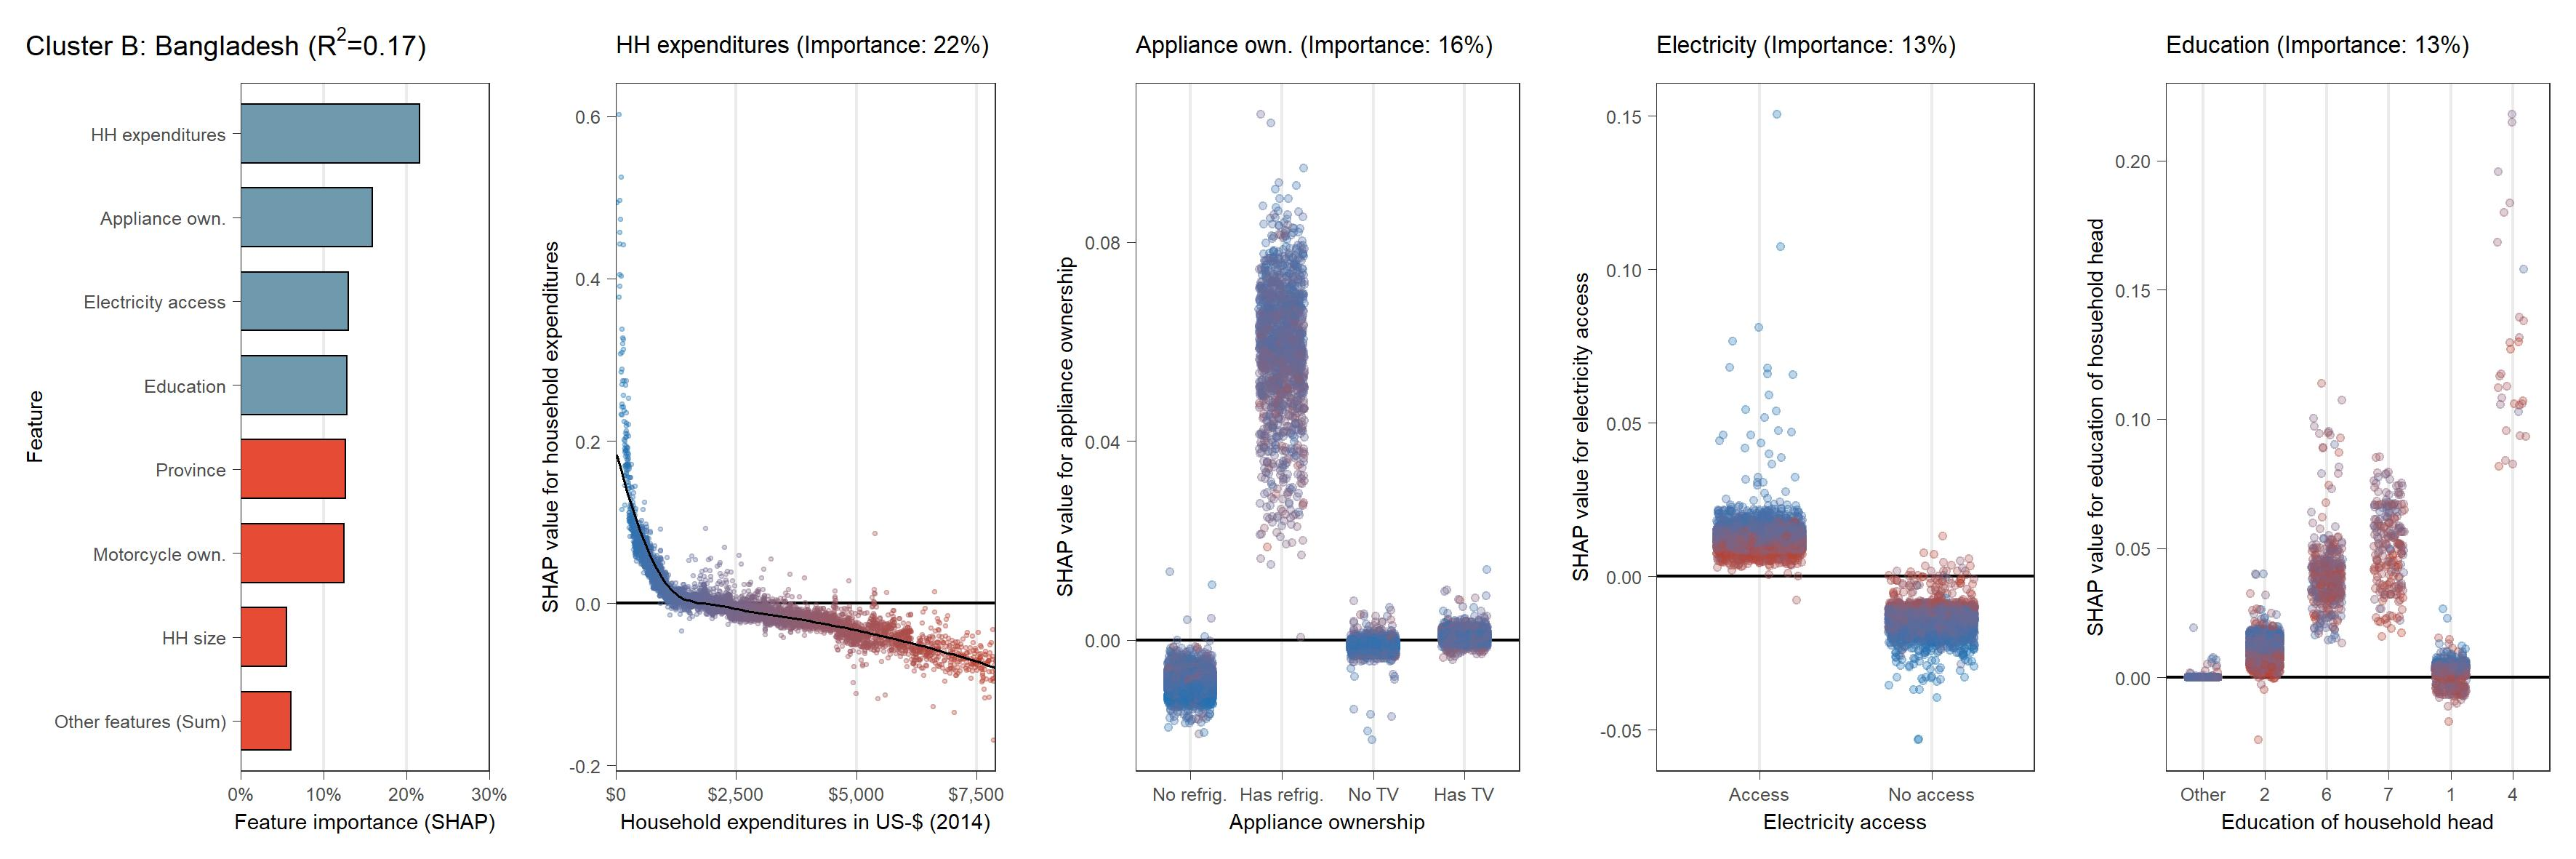
\includegraphics[width=\textwidth]{Figure 5b/Figure_5b_BGD} 
         \end{subfigure}
    \\
    \vspace{0.5cm}
   \begin{subfigure}[b]{\textwidth}        
   \centering
         \caption{Partial dependence plot (SHAP) for Côte d'Ivoire (cluster B)}
         \label{fig:5b_CIV}
         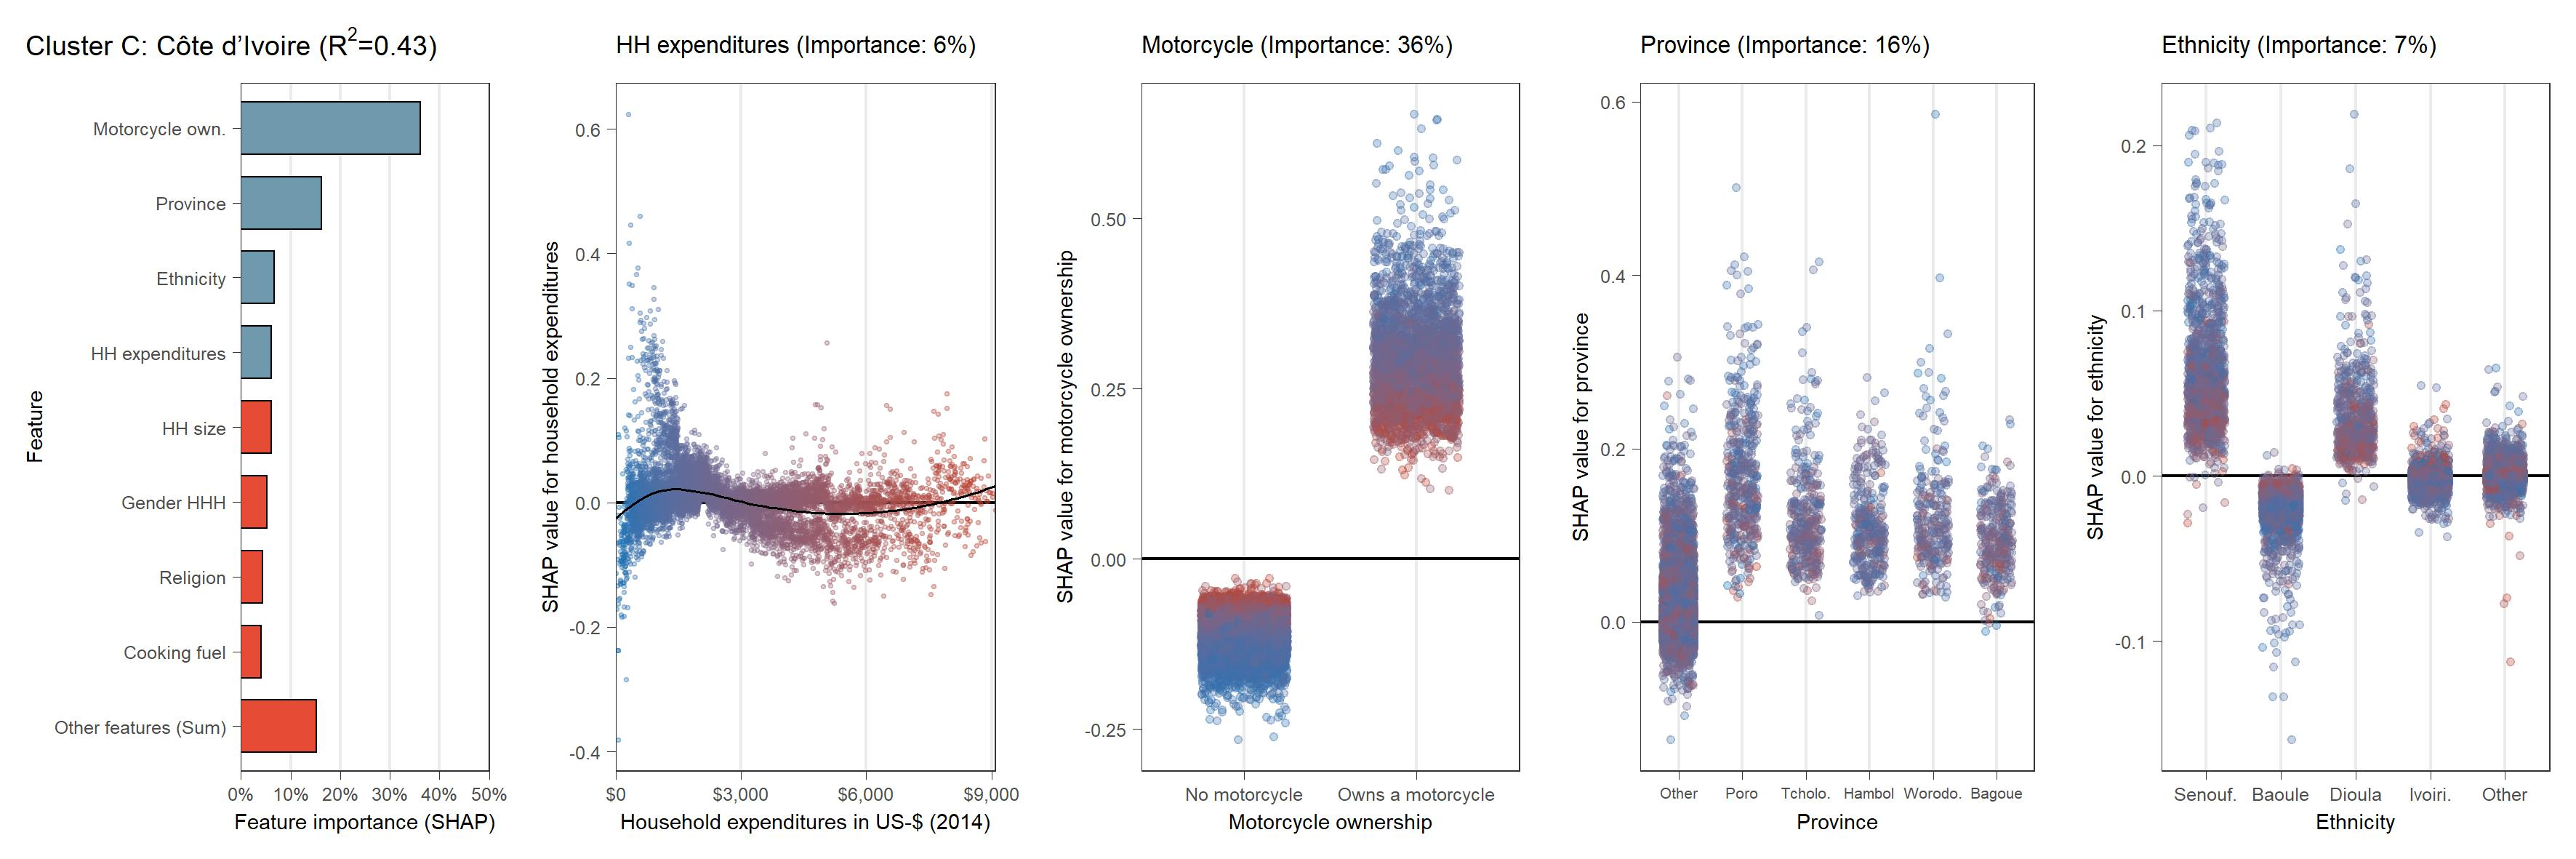
\includegraphics[width=\textwidth]{Figure 5b/Figure_5b_CIV}
         \end{subfigure}
    \\
    \vspace{0.5cm}
   \begin{subfigure}[b]{\textwidth}
   \centering
         \caption{Partial dependence plot (SHAP) for Ghana (cluster B)}
         \label{fig:5b_GHA}
         \includegraphics[width=\textwidth]{Figure 5b/Figure_5b_GHA}
         \end{subfigure}
    \\
    \vspace{0.5cm}
    \begin{subcaption2}
     This figure shows SHAP-values for predicting carbon intensity over feature values for 87 countries in order of nine country-clusters and silhouette width. The bar chart displays normalized average absolute SHAP-values for all features. Features with less than 3\% of normalized SHAP-values are subsumed as "Other features (Sum)". Charts show SHAP-values over total household expenditures for all countries and for the three most important features in each country besides total household expenditures. Colors represent household expenditures with blue (red) colors indicating lower (higher) household expenditures.
     \end{subcaption2}
\end{figure}

\begin{figure}[ht!]\ContinuedFloat
    \centering
   \begin{subfigure}[b]{\textwidth}
           \centering
         \caption{Partial dependence plot (SHAP) for Guinea-Bissau (cluster B)}
         \label{fig:5b_GNB}
         \includegraphics[width=\textwidth]{Figure 5b/Figure_5b_GNB}
         \end{subfigure}
    \\
    \vspace{0.5cm}
   \begin{subfigure}[b]{\textwidth}
   \centering
         \caption{Partial dependence plot (SHAP) for Guatemala (cluster B)}
         \label{fig:5b_GTM}
         \includegraphics[width=\textwidth]{Figure 5b/Figure_5b_GTM}
     \end{subfigure}
    \\
    \vspace{0.5cm}
   \begin{subfigure}[b]{\textwidth}
   \centering
         \caption{Partial dependence plot (SHAP) for Liberia (cluster B)}
         \label{fig:5b_LBR}
         \includegraphics[width=\textwidth]{Figure 5b/Figure_5b_LBR}
         \end{subfigure}
    \\
    \vspace{0.5cm}
    \begin{subcaption2}
     This figure shows SHAP-values for predicting carbon intensity over feature values for 87 countries in order of nine country-clusters and silhouette width. The bar chart displays normalized average absolute SHAP-values for all features. Features with less than 3\% of normalized SHAP-values are subsumed as "Other features (Sum)". Charts show SHAP-values over total household expenditures for all countries and for the three most important features in each country besides total household expenditures. Colors represent household expenditures with blue (red) colors indicating lower (higher) household expenditures.
     \end{subcaption2}
\end{figure}

\begin{figure}[ht!]\ContinuedFloat
    \centering
   \begin{subfigure}[b]{\textwidth}
  \centering
         \caption{Partial dependence plot (SHAP) for Mali (cluster B)}
         \label{fig:5b_MLI}
         \includegraphics[width=\textwidth]{Figure 5b/Figure_5b_MLI} \end{subfigure}
    \\
    \vspace{0.5cm}
   \begin{subfigure}[b]{\textwidth}
    \centering
         \caption{Partial dependence plot (SHAP) for Myanmar (cluster B)}
         \label{fig:5b_MMR}
         \includegraphics[width=\textwidth]{Figure 5b/Figure_5b_MMR}         
     \end{subfigure}
    \\
    \vspace{0.5cm}
   \begin{subfigure}[b]{\textwidth}
   \centering
         \caption{Partial dependence plot (SHAP) for Mozambique (cluster B)}
         \label{fig:5b_MOZ}
         \includegraphics[width=\textwidth]{Figure 5b/Figure_5b_MOZ}
         \end{subfigure}
    \\
    \vspace{0.5cm}
    \begin{subcaption2}
     This figure shows SHAP-values for predicting carbon intensity over feature values for 87 countries in order of nine country-clusters and silhouette width. The bar chart displays normalized average absolute SHAP-values for all features. Features with less than 3\% of normalized SHAP-values are subsumed as "Other features (Sum)". Charts show SHAP-values over total household expenditures for all countries and for the three most important features in each country besides total household expenditures. Colors represent household expenditures with blue (red) colors indicating lower (higher) household expenditures.
     \end{subcaption2}
\end{figure}

\begin{figure}[ht!]\ContinuedFloat
    \centering
   \begin{subfigure}[b]{\textwidth}
    \centering
         \caption{Partial dependence plot (SHAP) for Malawi (cluster B)}
         \label{fig:5b_MWI}
         \includegraphics[width=\textwidth]{Figure 5b/Figure_5b_MWI}
         \end{subfigure}
    \\
    \vspace{0.5cm}
   \begin{subfigure}[b]{\textwidth}
    \centering
         \caption{Partial dependence plot (SHAP) for Niger (cluster B)}
         \label{fig:5b_NER}
         \includegraphics[width=\textwidth]{Figure 5b/Figure_5b_NER} 
         \end{subfigure}
    \\
    \vspace{0.5cm}
   \begin{subfigure}[b]{\textwidth}
   \centering
         \caption{Partial dependence plot (SHAP) for Nigeria (cluster B)}
         \label{fig:5b_NGA}
         \includegraphics[width=\textwidth]{Figure 5b/Figure_5b_NGA}
         \end{subfigure}
    \\
    \vspace{0.5cm}
    \begin{subcaption2}
     This figure shows SHAP-values for predicting carbon intensity over feature values for 87 countries in order of nine country-clusters and silhouette width. The bar chart displays normalized average absolute SHAP-values for all features. Features with less than 3\% of normalized SHAP-values are subsumed as "Other features (Sum)". Charts show SHAP-values over total household expenditures for all countries and for the three most important features in each country besides total household expenditures. Colors represent household expenditures with blue (red) colors indicating lower (higher) household expenditures.
     \end{subcaption2}
\end{figure}

\begin{figure}[ht!]\ContinuedFloat
    \centering
   \begin{subfigure}[b]{\textwidth}
    \centering
         \caption{Partial dependence plot (SHAP) for Nicaragua (cluster B)}
         \label{fig:5b_NIC}
         \includegraphics[width=\textwidth]{Figure 5b/Figure_5b_NIC}    
         \end{subfigure}
    \\
    \vspace{0.5cm}
   \begin{subfigure}[b]{\textwidth}
   \centering
         \caption{Partial dependence plot (SHAP) for Pakistan (cluster B)}
         \label{fig:5b_PAK}
         \includegraphics[width=\textwidth]{Figure 5b/Figure_5b_PAK}   
         \end{subfigure}
    \\
    \vspace{0.5cm}
   \begin{subfigure}[b]{\textwidth}
   \centering
         \caption{Partial dependence plot (SHAP) for Paraguay (cluster B)}
         \label{fig:5b_PRY}
         \includegraphics[width=\textwidth]{Figure 5b/Figure_5b_PRY}
         \end{subfigure}
    \\
    \vspace{0.5cm}
    \begin{subcaption2}
     This figure shows SHAP-values for predicting carbon intensity over feature values for 87 countries in order of nine country-clusters and silhouette width. The bar chart displays normalized average absolute SHAP-values for all features. Features with less than 3\% of normalized SHAP-values are subsumed as "Other features (Sum)". Charts show SHAP-values over total household expenditures for all countries and for the three most important features in each country besides total household expenditures. Colors represent household expenditures with blue (red) colors indicating lower (higher) household expenditures.
     \end{subcaption2}
\end{figure}

\begin{figure}[ht!]\ContinuedFloat
    \centering
   \begin{subfigure}[b]{\textwidth}
   \centering
         \caption{Partial dependence plot (SHAP) for Senegal (cluster B)}
         \label{fig:5b_SEN}
         \includegraphics[width=\textwidth]{Figure 5b/Figure_5b_SEN}  
         \end{subfigure}
    \\
    \vspace{0.5cm}
   \begin{subfigure}[b]{\textwidth}    
   \centering
         \caption{Partial dependence plot (SHAP) for Togo (cluster B)}
         \label{fig:5b_TGO}
         \includegraphics[width=\textwidth]{Figure 5b/Figure_5b_TGO}    
   \end{subfigure}
    \\
    \vspace{0.5cm}
   \begin{subfigure}[b]{\textwidth} 
   \centering
         \caption{Partial dependence plot (SHAP) for Dominican Republic (cluster C)}
         \label{fig:5b_DOM}
         \includegraphics[width=\textwidth]{Figure 5b/Figure_5b_DOM}
         \end{subfigure}
    \\
    \vspace{0.5cm}
    \begin{subcaption2}
     This figure shows SHAP-values for predicting carbon intensity over feature values for 87 countries in order of nine country-clusters and silhouette width. The bar chart displays normalized average absolute SHAP-values for all features. Features with less than 3\% of normalized SHAP-values are subsumed as "Other features (Sum)". Charts show SHAP-values over total household expenditures for all countries and for the three most important features in each country besides total household expenditures. Colors represent household expenditures with blue (red) colors indicating lower (higher) household expenditures.
     \end{subcaption2}
\end{figure}

\begin{figure}[ht!]\ContinuedFloat
    \centering
   \begin{subfigure}[b]{\textwidth}
    \centering
         \caption{Partial dependence plot (SHAP) for Egypt (cluster C)}
         \label{fig:5b_EGY}
         \includegraphics[width=\textwidth]{Figure 5b/Figure_5b_EGY}    
   \end{subfigure}
    \\
    \vspace{0.5cm}
   \begin{subfigure}[b]{\textwidth}
   \centering
         \caption{Partial dependence plot (SHAP) for Georgia (cluster C)}
         \label{fig:5b_GEO}
         \includegraphics[width=\textwidth]{Figure 5b/Figure_5b_GEO}    
   \end{subfigure}
    \\
    \vspace{0.5cm}
   \begin{subfigure}[b]{\textwidth} 
   \centering
         \caption{Partial dependence plot (SHAP) for Indonesia (cluster C)}
         \label{fig:5b_IDN}
         \includegraphics[width=\textwidth]{Figure 5b/Figure_5b_IDN}
    \end{subfigure}
    \\
    \vspace{0.5cm}
    \begin{subcaption2}
     This figure shows SHAP-values for predicting carbon intensity over feature values for 87 countries in order of nine country-clusters and silhouette width. The bar chart displays normalized average absolute SHAP-values for all features. Features with less than 3\% of normalized SHAP-values are subsumed as "Other features (Sum)". Charts show SHAP-values over total household expenditures for all countries and for the three most important features in each country besides total household expenditures. Colors represent household expenditures with blue (red) colors indicating lower (higher) household expenditures.
     \end{subcaption2}
\end{figure}

\begin{figure}[ht!]\ContinuedFloat
    \centering
   \begin{subfigure}[b]{\textwidth}
    \centering
         \caption{Partial dependence plot (SHAP) for India (cluster C)}
         \label{fig:5b_IND}
         \includegraphics[width=\textwidth]{Figure 5b/Figure_5b_IND}    
    \end{subfigure}
    \\
    \vspace{0.5cm}
   \begin{subfigure}[b]{\textwidth}  
   \centering
         \caption{Partial dependence plot (SHAP) for Jordan (cluster C)}
         \label{fig:5b_JOR}
         \includegraphics[width=\textwidth]{Figure 5b/Figure_5b_JOR}
    \end{subfigure}
    \\
    \vspace{0.5cm}
   \begin{subfigure}[b]{\textwidth}
    \centering
         \caption{Partial dependence plot (SHAP) for Mexico (cluster C)}
         \label{fig:5b_MEX}
         \includegraphics[width=\textwidth]{Figure 5b/Figure_5b_MEX}
         \end{subfigure}
    \\
    \vspace{0.5cm}
    \begin{subcaption2}
     This figure shows SHAP-values for predicting carbon intensity over feature values for 87 countries in order of nine country-clusters and silhouette width. The bar chart displays normalized average absolute SHAP-values for all features. Features with less than 3\% of normalized SHAP-values are subsumed as "Other features (Sum)". Charts show SHAP-values over total household expenditures for all countries and for the three most important features in each country besides total household expenditures. Colors represent household expenditures with blue (red) colors indicating lower (higher) household expenditures.
     \end{subcaption2}
\end{figure}

\begin{figure}[ht!]\ContinuedFloat
    \centering
   \begin{subfigure}[b]{\textwidth}
   \centering
         \caption{Partial dependence plot (SHAP) for Philippines (cluster C)}
         \label{fig:5b_PHL}
         \includegraphics[width=\textwidth]{Figure 5b/Figure_5b_PHL}    
         \end{subfigure}
    \\
    \vspace{0.5cm}
   \begin{subfigure}[b]{\textwidth}
   \centering
         \caption{Partial dependence plot (SHAP) for Russian Federation (cluster C)}
         \label{fig:5b_RUS}
         \includegraphics[width=\textwidth]{Figure 5b/Figure_5b_RUS} 
    \end{subfigure}
    \\
    \vspace{0.5cm}
   \begin{subfigure}[b]{\textwidth}
   \centering
         \caption{Partial dependence plot (SHAP) for Thailand (cluster C)}
         \label{fig:5b_THA}
         \includegraphics[width=\textwidth]{Figure 5b/Figure_5b_THA} 
   \end{subfigure}
    \\
    \vspace{0.5cm}
    \begin{subcaption2}
     This figure shows SHAP-values for predicting carbon intensity over feature values for 87 countries in order of nine country-clusters and silhouette width. The bar chart displays normalized average absolute SHAP-values for all features. Features with less than 3\% of normalized SHAP-values are subsumed as "Other features (Sum)". Charts show SHAP-values over total household expenditures for all countries and for the three most important features in each country besides total household expenditures. Colors represent household expenditures with blue (red) colors indicating lower (higher) household expenditures.
     \end{subcaption2}
\end{figure}

\begin{figure}[ht!]\ContinuedFloat
    \centering
   \begin{subfigure}[b]{\textwidth}
   \centering
         \caption{Partial dependence plot (SHAP) for Taiwan (cluster C)}
         \label{fig:5b_TWN}
         \includegraphics[width=\textwidth]{Figure 5b/Figure_5b_TWN}    
   \end{subfigure}
    \\
    \vspace{0.5cm}
   \begin{subfigure}[b]{\textwidth} 
   \centering
         \caption{Partial dependence plot (SHAP) for Vietnam (cluster C)}
         \label{fig:5b_VNM}
         \includegraphics[width=\textwidth]{Figure 5b/Figure_5b_VNM}    
   \end{subfigure}
    \\
    \vspace{0.5cm}
   \begin{subfigure}[b]{\textwidth}  
   \centering
         \caption{Partial dependence plot (SHAP) for South Africa (cluster C)}
         \label{fig:5b_ZAF}
         \includegraphics[width=\textwidth]{Figure 5b/Figure_5b_ZAF}    
    \end{subfigure}
    \\
    \vspace{0.5cm}
    \begin{subcaption2}
     This figure shows SHAP-values for predicting carbon intensity over feature values for 87 countries in order of nine country-clusters and silhouette width. The bar chart displays normalized average absolute SHAP-values for all features. Features with less than 3\% of normalized SHAP-values are subsumed as "Other features (Sum)". Charts show SHAP-values over total household expenditures for all countries and for the three most important features in each country besides total household expenditures. Colors represent household expenditures with blue (red) colors indicating lower (higher) household expenditures.
     \end{subcaption2}
\end{figure}

\begin{figure}[ht!]\ContinuedFloat
    \centering
   \begin{subfigure}[b]{\textwidth}
   \centering
         \caption{Partial dependence plot (SHAP) for Bolivia (cluster D)}
         \label{fig:5b_BOL}
         \includegraphics[width=\textwidth]{Figure 5b/Figure_5b_BOL}
         \end{subfigure}
    \\
    \vspace{0.5cm}
   \begin{subfigure}[b]{\textwidth}        
    \centering
         \caption{Partial dependence plot (SHAP) for Ecuador (cluster D)}
         \label{fig:5b_ECU}
         \includegraphics[width=\textwidth]{Figure 5b/Figure_5b_ECU}
    \end{subfigure}
    \\
    \vspace{0.5cm}
   \begin{subfigure}[b]{\textwidth}
    \centering
         \caption{Partial dependence plot (SHAP) for Iraq (cluster D)}
         \label{fig:5b_IRQ}
         \includegraphics[width=\textwidth]{Figure 5b/Figure_5b_IRQ}
         \end{subfigure}
    \\
    \vspace{0.5cm}
    \begin{subcaption2}
     This figure shows SHAP-values for predicting carbon intensity over feature values for 87 countries in order of nine country-clusters and silhouette width. The bar chart displays normalized average absolute SHAP-values for all features. Features with less than 3\% of normalized SHAP-values are subsumed as "Other features (Sum)". Charts show SHAP-values over total household expenditures for all countries and for the three most important features in each country besides total household expenditures. Colors represent household expenditures with blue (red) colors indicating lower (higher) household expenditures.
     \end{subcaption2}
\end{figure}


\begin{figure}[ht!]\ContinuedFloat
    \centering
   \begin{subfigure}[b]{\textwidth}
     \centering
         \caption{Partial dependence plot (SHAP) for Peru (cluster D)}
         \label{fig:5b_PER}
         \includegraphics[width=\textwidth]{Figure 5b/Figure_5b_PER}        
     \end{subfigure}
    \\
    \vspace{0.5cm}
   \begin{subfigure}[b]{\textwidth}
    \centering
         \caption{Partial dependence plot (SHAP) for El Salvador (cluster D)}
         \label{fig:5b_SLV}
         \includegraphics[width=\textwidth]{Figure 5b/Figure_5b_SLV} 
    \end{subfigure}
    \\
    \vspace{0.5cm}
   \begin{subfigure}[b]{\textwidth}     
    \centering
         \caption{Partial dependence plot (SHAP) for Armenia (cluster E)}
         \label{fig:5b_ARM}
         \includegraphics[width=\textwidth]{Figure 5b/Figure_5b_ARM}     
    \end{subfigure}
    \\
    \vspace{0.5cm}
    \begin{subcaption2}
     This figure shows SHAP-values for predicting carbon intensity over feature values for 87 countries in order of nine country-clusters and silhouette width. The bar chart displays normalized average absolute SHAP-values for all features. Features with less than 3\% of normalized SHAP-values are subsumed as "Other features (Sum)". Charts show SHAP-values over total household expenditures for all countries and for the three most important features in each country besides total household expenditures. Colors represent household expenditures with blue (red) colors indicating lower (higher) household expenditures.
     \end{subcaption2}
\end{figure}

\begin{figure}[ht!]\ContinuedFloat
    \centering
   \begin{subfigure}[b]{\textwidth}
     \centering
         \caption{Partial dependence plot (SHAP) for Turkey (cluster E)}
         \label{fig:5b_TUR}
         \includegraphics[width=\textwidth]{Figure 5b/Figure_5b_TUR}      
        \end{subfigure}
    \\
    \vspace{0.5cm}
   \begin{subfigure}[b]{\textwidth}
   \centering
         \caption{Partial dependence plot (SHAP) for Rwanda (cluster F)}
         \label{fig:5b_RWA}
         \includegraphics[width=\textwidth]{Figure 5b/Figure_5b_RWA}          
     \end{subfigure}
    \\
    \vspace{0.5cm}
   \begin{subfigure}[b]{\textwidth} 
   \centering
         \caption{Partial dependence plot (SHAP) for Uganda (cluster F)}
         \label{fig:5b_UGA}
         \includegraphics[width=\textwidth]{Figure 5b/Figure_5b_UGA}
    \end{subfigure}
    \\
    \vspace{0.5cm}

    \begin{subcaption2}
     This figure shows SHAP-values for predicting carbon intensity over feature values for 87 countries in order of nine country-clusters and silhouette width. The bar chart displays normalized average absolute SHAP-values for all features. Features with less than 3\% of normalized SHAP-values are subsumed as "Other features (Sum)". Charts show SHAP-values over total household expenditures for all countries and for the three most important features in each country besides total household expenditures. Colors represent household expenditures with blue (red) colors indicating lower (higher) household expenditures.
     \end{subcaption2}
\end{figure}